% !TeX spellcheck = en-US
% !TeX encoding = utf8
% !TeX program = pdflatex
% !BIB program = biber
% -*- coding:utf-8 mod:LaTeX -*-


% vv  scroll down to line 200 for content  vv


\let\ifdeutsch\iffalse
\let\ifenglisch\iftrue
% EN: This file is loaded before the \documentclass command in the main document

% EN: The following package allows \\ at the title page
%     For more information see https://github.com/latextemplates/scientific-thesis-cover/issues/4
\RequirePackage{kvoptions-patch}

\ifenglisch
  \PassOptionsToClass{numbers=noenddot}{scrbook}
\else
  %()Aus scrguide.pdf - der Dokumentation von KOMA-Script)
  %Nach DUDEN steht in Gliederungen, in denen ausschließlich arabische Ziffern für die Nummerierung
  %verwendet werden, am Ende der Gliederungsnummern kein abschließender Punkt
  %(siehe [DUD96, R3]). Wird hingegen innerhalb der Gliederung auch mit römischen Zahlen
  %oder Groß- oder Kleinbuchstaben gearbeitet, so steht am Ende aller Gliederungsnummern ein
  %abschließender Punkt (siehe [DUD96, R4])
  \PassOptionsToClass{numbers=autoendperiod}{scrbook}
\fi

% Warns about outdated packages and missing caption declarations
% See https://www.ctan.org/pkg/nag
\RequirePackage[l2tabu, orthodox]{nag}

%DE: Neue deutsche Trennmuster
%    Siehe http://www.ctan.org/pkg/dehyph-exptl und http://projekte.dante.de/Trennmuster/WebHome
%    Nur für pdflatex, nicht für lualatex
\RequirePackage{ifluatex}
\ifluatex
  % do not load anything
\else
  \ifdeutsch
    \RequirePackage[ngerman=ngerman-x-latest]{hyphsubst}
  \fi
\fi

\documentclass[
  % fontsize=11pt is the standard
  a4paper,  % Standard format - only KOMAScript uses paper=a4 - https://tex.stackexchange.com/a/61044/9075
  twoside,  % we are optimizing for both screen and two-side printing. So the page numbers will jump, but the content is configured to stay in the middle (by using the geometry package)
  bibliography=totoc,
  %               idxtotoc,   %Index ins Inhaltsverzeichnis
  %               liststotoc, %List of X ins Inhaltsverzeichnis, mit liststotocnumbered werden die Abbildungsverzeichnisse nummeriert
  headsepline,
  cleardoublepage=empty,
  parskip=half,
  %               draft    % um zu sehen, wo noch nachgebessert werden muss - wichtig, da Bindungskorrektur mit drin
  draft=false
]{scrbook}
% !TeX encoding = utf8
% -*- coding:utf-8 mod:LaTeX -*-

% EN: This file includes basic packages and sets options. The order of package
%     loading is important

% DE: In dieser Datei werden zuerst die benoetigten Pakete eingebunden und
%     danach diverse Optionen gesetzt. Achtung Reihenfolge ist entscheidend!


% EN: Styleguide:
% - English comments are prefixed with "EN", German comments are prefixed with "DE"
% - Prefixed headings define the language for the subsequent paragraphs
% - It is tried to organize packages in blocks. Bocks are separated by two empty lines.

% DE: Styleguide:
%
% Ein sehr kleiner Styleguide. Packages werden in Blöcken organisiert.
% Zwischen zwei Blöcken sind 2 Leerzeilen!


% EN: Enable copy and paste of text from the PDF
%     Only required for pdflatex. It "just works" in the case of lualatex.
%     mmap enables mathematical symbols, but does not work with the newtx font set
%     See: https://tex.stackexchange.com/a/64457/9075
%     Other solutions outlined at http://goemonx.blogspot.de/2012/01/pdflatex-ligaturen-und-copynpaste.html and http://tex.stackexchange.com/questions/4397/make-ligatures-in-linux-libertine-copyable-and-searchable
%     Trouble shooting outlined at https://tex.stackexchange.com/a/100618/9075

\ifluatex
\else
  \usepackage{cmap}
\fi


% EN: File encoding
% DE: Codierung
%     Wir sind im 21 Jahrhundert, utf-8 löst so viele Probleme.
%
% Mit UTF-8 funktionieren folgende Pakete nicht mehr. Bitte beachten!
%   * fancyvrb mit §
%   * easylist -> http://www.ctan.org/tex-archive/macros/latex/contrib/easylist/
\ifluatex
  % EN: See https://tex.stackexchange.com/a/158517/9075
  %     Not required, because of usage of fontspec package
  %\usepackage[utf8]{luainputenc}
\else
  \usepackage[utf8]{inputenc}
\fi


% DE: Parallelbetrieb tex4ht und pdflatex

\makeatletter
\@ifpackageloaded{tex4ht}{
  \def\iftex4ht{\iftrue}
}{
  \def\iftex4ht{\iffalse}
}
\makeatother


% EN: Mathematics
% DE: Mathematik
%
% DE: Viele Mathematik-Sachen. Siehe https://texdoc.net/pkg/amsmath
%
% EN: Options must be passed this way, otherwise it does not work with glossaries
% DE: fleqn (=Gleichungen linksbündig platzieren) funktioniert nicht direkt. Es muss noch ein Patch gemacht werden:
\PassOptionsToPackage{leqno}{amsmath}
%
% DE: amsmath Muss nicht mehr geladen werden, da es von newtxmath automatisch geladen wird
% \usepackage{amsmath}


%% EN: Fonts
%% DE: Schriften
%%
%% !!! If you change the font, be sure that words such as "workflow" can
%% !!! still be copied from the PDF. If this is not the case, you have
%% !!! to use glyphtounicode. See comment at cmap package


% EN: Times Roman for all text
\ifluatex
  % source: Second proposed fix from the following answer: https://tex.stackexchange.com/a/394137
  \usepackage[no-math]{fontspec}
  \setmainfont{TeXGyreTermes-Regular}[
       BoldFont       = TeXGyreTermes-Bold ,
       ItalicFont     = TeXGyreTermes-Italic ,
       BoldItalicFont = TeXGyreTermes-BoldItalic,
       NFSSFamily     = ntxtlf]
  \setsansfont{TeX Gyre Heros Regular}[
       Scale=.9,
       BoldFont       = TeX Gyre Heros Bold,
       ItalicFont     = TeX Gyre Heros Italic,
       BoldItalicFont = TeX Gyre Heros BoldItalic]
  \setmonofont[StylisticSet={1,3},Scale=.9]{inconsolata}
  \RequirePackage{newtxmath}
\else
  \RequirePackage{newtxtext}
  \RequirePackage{newtxmath}
  % EN: looks good with times, but no equivalent for lualatex found,
  %     therefore replaced with inconsolata
  %\RequirePackage[zerostyle=b,scaled=.9]{newtxtt}
  \RequirePackage[varl,scaled=.9]{inconsolata}
\fi

% EN: Fallback font - if the subsequent font packages do not define a font (e.g., monospaced)
%     This is the modern package for "Computer Modern".
%     In case this gets activated, one has to switch from cmap package to glyphtounicode (in the case of pdflatex)
% DE: Fallback-Schriftart
%\usepackage[%
%    rm={oldstyle=false,proportional=true},%
%    sf={oldstyle=false,proportional=true},%
%    tt={oldstyle=false,proportional=true,variable=true},%
%    qt=false%
%]{cfr-lm}

% EN: Headings are typset in Helvetica (which is similar to Arial)
% DE: Schriftart fuer die Ueberschriften - ueberschreibt lmodern
%\usepackage[scaled=.95]{helvet}

% DE: Für Schreibschrift würde tun, muss aber nicht
%\usepackage{mathrsfs} %  \mathscr{ABC}

% EN: Font for the main text
% DE: Schriftart fuer den Fliesstext - ueberschreibt lmodern
%     Linux Libertine, siehe http://www.linuxlibertine.org/
%     Packageparamter [osf] = Minuskel-Ziffern
%     rm = libertine im Brottext, Linux Biolinum NICHT als serifenlose Schrift, sondern helvet (von oben) beibehalten
%\usepackage[rm]{libertine}

% EN: Alternative Font: Palantino. It is recommeded by Prof. Ludewig for German texts
% DE: Alternative Schriftart: Palantino, Packageparamter [osf] = Minuskel-Ziffern
%     Bitte nur in deutschen Texten
%\usepackage{mathpazo} %ftp://ftp.dante.de/tex-archive/fonts/mathpazo/ - Tipp aus DE-TEX-FAQ 8.2.1

% DE: Schriftart fuer Programmcode - ueberschreibt lmodern
%     Falls auskommentiert, wird die Standardschriftart lmodern genommen
%     Fuer schreibmaschinenartige Schluesselwoerter in den Listings - geht bei alten Installationen nicht, da einige Fontshapes (<>=) fehlen
%\usepackage[scaled=.92]{luximono}
%\usepackage{courier}
% DE: BeraMono als Typewriter-Schrift, Tipp von http://tex.stackexchange.com/a/71346/9075
%\usepackage[scaled=0.83]{beramono}

% EN: backticks (`) are rendered as such in verbatim environments.
%     See following links for details:
%     - https://tex.stackexchange.com/a/341057/9075
%     - https://tex.stackexchange.com/a/47451/9075
%     - https://tex.stackexchange.com/a/166791/9075
\usepackage{upquote}

% DE: Symbole
%
%\usepackage[geometry]{ifsym} % \BigSquare
%\usepackage{mathabx}
%\usepackage{stmaryrd} %fuer \ovee, \owedge, \otimes
%\usepackage{marvosym} %fuer \Writinghand %patched to not redefine \Rightarrow
%\usepackage{mathrsfs} %mittels \mathscr{} schoenen geschwungenen Buchstaben erzeugen
%\usepackage{calrsfs} %\mathcal{} ein bisserl dickeren buchstaben erzeugen - sieht net so gut aus.
%durch mathpazo ist das schon definiert

%
%\usepackage{amssymb}

% EN: For \texttrademark{}
\usepackage{textcomp}

% EN: name-clashes von marvosym und mathabx vermeiden:
\def\delsym#1{%
  %  \expandafter\let\expandafter\origsym\expandafter=\csname#1\endcsname
  %  \expandafter\let\csname orig#1\endcsname=\origsym
  \expandafter\let\csname#1\endcsname=\relax
}

%\usepackage{pifont}
%\usepackage{bbding}
%\delsym{Asterisk}
%\delsym{Sun}\delsym{Mercury}\delsym{Venus}\delsym{Earth}\delsym{Mars}
%\delsym{Jupiter}\delsym{Saturn}\delsym{Uranus}\delsym{Neptune}
%\delsym{Pluto}\delsym{Aries}\delsym{Taurus}\delsym{Gemini}
%\delsym{Rightarrow}
%\usepackage{mathabx} - Ueberschreibt leider zu viel - und die \le-Zeichen usw. sehen nicht gut aus!


% EN: Modern font encoding
%     Has to be loaded AFTER any font packages. See https://tex.stackexchange.com/a/2869/9075.
\ifluatex
\else
  \usepackage[T1]{fontenc}
\fi
%


% EN: Character protrusion and font expansion. See http://www.ctan.org/tex-archive/macros/latex/contrib/microtype/
% DE: Optischer Randausgleich und Grauwertkorrektur

\usepackage[
  babel=true, % EN: Enable language-specific kerning. Take language-settings from the languge of the current document (see Section 6 of microtype.pdf)
  expansion=alltext,
  protrusion=alltext-nott, % EN: Ensure that at listings, there is no change at the margin of the listing
  final % EN: Always enable microtype, even if in draft mode. This helps finding bad boxes quickly.
        %     In the standard configuration, this template is always in the final mode, so this option only makes a difference if "pros" use the draft mode
]{microtype}


% EN: \texttt{test -- test} keeps the "--" as "--" (and does not convert it to an en dash)
\DisableLigatures{encoding = T1, family = tt* }

% DE: fuer microtype
% DE: tracking=true muss als Parameter des microtype-packages mitgegeben werden
% DE: Deaktiviert, da dies bei Algorithmen seltsam aussieht

%\DeclareMicrotypeSet*[tracking]{my}{ font = */*/*/sc/* }%
%\SetTracking{ encoding = *, shape = sc }{ 45 }
% DE: Hier wird festgelegt,
%     dass alle Passagen in Kapitälchen automatisch leicht
%     gesperrt werden.
%     Quelle: http://homepage.ruhr-uni-bochum.de/Georg.Verweyen/pakete.html
%    Deaktiviert, da sonst "BPEL", "BPMN" usw. wirklich komisch aussehen.
%     Macht wohl nur bei geisteswissenschaftlichen Arbeiten Sinn.


% EN: amsmath teaks


% EN: Fixes bugs in AMS math
%     Corrently conflicts with unicode-math
% \usepackage{mathtools}

%\numberwithin{equation}{section}
%\renewcommand{\theequation}{\thesection.\Roman{equation}}

% EN: work-around ams-math problem with align and 9 -> 10. Does not work with glossaries, No visual changes.
%\addtolength\mathindent{1em}


% EN: For theorems, replacement for amsthm
\usepackage[amsmath,hyperref]{ntheorem}
\theorempreskipamount 2ex plus1ex minus0.5ex
\theorempostskipamount 2ex plus1ex minus0.5ex
\theoremstyle{break}
\newtheorem{definition}{Definition}[section]


% CTAN: https://ctan.org/pkg/lccaps
% Doc: http://texdoc.net/pkg/lccaps
%
% Required for DE/EN \initialism
\usepackage{lccaps}


% EN: Defintion of colors. Argument "hyperref" is not used as we do not want to change border colors of links: Links are not colored anymore.
% DE: Farbdefinitionen
\usepackage[dvipsnames]{xcolor}


% EN: Required for custom acronyms/glossaries style.
%     Left aligned Columns in tables with fixed width.
%     See http://tex.stackexchange.com/questions/91566/syntax-similar-to-centering-for-right-and-left
\usepackage{ragged2e}


% DE: Wichtig, ansonsten erscheint "No room for a new \write"
\usepackage{scrwfile}


% EN: Support for language-specific hyphenation
% DE: Neue deutsche Rechtschreibung und Literatur statt "Literature"
%     Die folgende Einstellung ist der Nachfolger von ngerman.sty
\ifdeutsch
  % DE: letzte Sprache ist default, Einbindung von "american" ermöglicht \begin{otherlanguage}{amercian}...\end{otherlanguage} oder \foreignlanguage{american}{Text in American}
  %     Siehe auch http://tex.stackexchange.com/a/50638/9075
  \usepackage[american,main=ngerman]{babel}
  % Ein "abstract" ist eine "Kurzfassung", keine "Zusammenfassung"
  \addto\captionsngerman{%
    \renewcommand\abstractname{Kurzfassung}%
  }
  \ifluatex
    % EN: conditionally disable ligatures. See https://github.com/latextemplates/scientific-thesis-template/issues/54
    %     for a discussion
    \usepackage[ngerman]{selnolig}
  \fi
\else
  % EN: Set English as language and allow to write hyphenated"=words
  %     `american`, `english` and `USenglish` are synonyms for babel package (according to https://tex.stackexchange.com/questions/12775/babel-english-american-usenglish).
  %      "english" has to go last to set it as default language
  \usepackage[ngerman,main=english]{babel}
  % EN: Hint by http://tex.stackexchange.com/a/321066/9075 -> enable "= as dashes
  \addto\extrasenglish{\languageshorthands{ngerman}\useshorthands{"}}
  \ifluatex
    % EN: conditionally disable ligatures. See https://github.com/latextemplates/scientific-thesis-template/issues/54
    %     for a discussion
    \usepackage[english]{selnolig}
  \fi
\fi
%


% EN: For easy quotations: \enquote{text}
%     This package is very smart when nesting is applied, otherwise textcmds (see below) provides a shorter command
%     Note that this package results in a warning when it is loaded before minted (actually fvextra).
% DE: Anführungszeichen
%     Zitate in \enquote{...} setzen, dann werden automatisch die richtigen Anführungszeichen verwendet.
%     Dieses package erzeugt eine Warnung, wenn es vor minted (genauer fvextra) geladen wird.
\usepackage{csquotes}


% EN: For even easier quotations: \qq{text}.
%     Is not smart in the case of nesting, but good enough for the most cases
\usepackage{textcmds}
\ifdeutsch
  % EN: German quotes are different. So do not use the English quotes, but the ones provided by the csquotes package.
  \renewcommand{\qq}[1]{\enquote{#1}}
\fi


% EN: extended enumarations
% DE: erweitertes Enumerate
\usepackage{paralist}


% DE: Gestaltung der Kopf- und Fußteilen

\usepackage[automark]{scrlayer-scrpage}

\automark[section]{chapter}
\setkomafont{pageheadfoot}{\normalfont\sffamily}
\setkomafont{pagenumber}{\normalfont\sffamily}

% DE: funktioniert nicht: Alle Linien sind hier weg
%\setheadsepline[.4pt]{.4pt}


% DE: Intelligentes Leerzeichen um hinter Abkürzungen die richtigen Abstände zu erhalten, auch leere.
%     Siehe commands.tex \gq{}
\usepackage{xspace}
% DE: Macht \xspace und \enquote kompatibel
\makeatletter
\xspaceaddexceptions{\grqq \grq \csq@qclose@i \} }
\makeatother


\newcommand{\eg}{e.\,g.,\ }
\newcommand{\ie}{i.\,e.,\ }


% EN: introduce \powerset - hint by http://matheplanet.com/matheplanet/nuke/html/viewtopic.php?topic=136492&post_id=997377
\DeclareFontFamily{U}{MnSymbolC}{}
\DeclareSymbolFont{MnSyC}{U}{MnSymbolC}{m}{n}
\DeclareFontShape{U}{MnSymbolC}{m}{n}{
  <-6>    MnSymbolC5
  <6-7>   MnSymbolC6
  <7-8>   MnSymbolC7
  <8-9>   MnSymbolC8
  <9-10>  MnSymbolC9
  <10-12> MnSymbolC10
  <12->   MnSymbolC12%
}{}
\DeclareMathSymbol{\powerset}{\mathord}{MnSyC}{180}


% EN: Package for the appendix
% DE: Anhang
\usepackage{appendix}
%[toc,page,title,header]
%


% EN: Graphics
% DE: Grafikeinbindungen
%
% EN: The parameter "pdftex" is not required
\usepackage{graphicx}
\graphicspath{{\getgraphicspath}}
\newcommand{\getgraphicspath}{graphics/}


% EN: Enables inclusion of SVG graphics - 1:1 approach
%    This is NOT the approach of https://ctan.org/pkg/svg-inkscape,
%     which allows text in SVG to be typeset using LaTeX
%     We just include the SVG as is.
\usepackage{epstopdf}
\epstopdfDeclareGraphicsRule{.svg}{pdf}{.pdf}{%
  inkscape -z -D --file=#1 --export-pdf=\OutputFile
}


% EN: Enables inclusion of SVG graphics - text-rendered-with-LaTeX-approach
%     This is the approach of https://ctan.org/pkg/svg-inkscape,
\newcommand{\executeiffilenewer}[3]{%
  \IfFileExists{#2}
  {
    %\message{file #2 exists}
    \ifnum\pdfstrcmp{\pdffilemoddate{#1}}%
      {\pdffilemoddate{#2}}>0%
      {\immediate\write18{#3}}
    \else
      {%\message{file up to date #2}
      }
    \fi%
  }{
    %\message{file #2 doesn't exist}
    %\message{argument: #3}
    %\immediate\write18{echo "test" > xoutput.txt}
    \immediate\write18{#3}
  }
}
\newcommand{\includesvg}[1]{%
  \executeiffilenewer{#1.svg}{#1.pdf}%
  {
    inkscape -z -D --file=\getgraphicspath#1.svg %
    --export-pdf=\getgraphicspath#1.pdf --export-latex}%
  \input{\getgraphicspath#1.pdf_tex}%
}


% EN: Enable typesetting values with SI units.
\ifdeutsch
  \usepackage[mode=text,group-four-digits]{siunitx}
  \sisetup{locale=DE}
\else
  \usepackage[mode=text,group-four-digits,group-separator={,}]{siunitx}
  \sisetup{locale=US}
\fi


% EN: Extensions for tables
% DE: Tabellenerweiterungen
\usepackage{array} %increases tex's buffer size and enables ``>'' in tablespecs
\usepackage{longtable}
\usepackage{dcolumn} %Aligning numbers by decimal points in table columns
\ifdeutsch
  \newcolumntype{d}[1]{D{.}{,}{#1}}
\else
  \newcolumntype{d}[1]{D{.}{.}{#1}}
\fi
\setlength{\extrarowheight}{1pt}


% DE: Eine Zelle, die sich über mehrere Zeilen erstreckt.
%     Siehe Beispieltabelle in Kapitel 2
\usepackage{multirow}


% DE: Fuer Tabellen mit Variablen Spaltenbreiten
%\usepackage{tabularx}
%\usepackage{tabulary}


% EN: Links behave as they should. Enables "\url{...}" for URL typesettings.
%     Allow URL breaks also at a hyphen, even though it might be confusing: Is the "-" part of the address or just a hyphen?
%     See https://tex.stackexchange.com/a/3034/9075.
% DE: Links verhalten sich so, wie sie sollen
%     Zeilenumbrüche bei URLs auch bei Bindestrichen erlauben, auch wenn es verwirrend sein könnte: Gehört der Bindestrich zur URL oder ist es ein Trennstrich?
%     Siehe https://tex.stackexchange.com/a/3034/9075.
\usepackage[hyphens]{url}
%
%  EN: When activated, use text font as url font, not the monospaced one.
%      For all options see https://tex.stackexchange.com/a/261435/9075.
% \urlstyle{same}
%
% EN: Hint by http://tex.stackexchange.com/a/10419/9075.
\makeatletter
\g@addto@macro{\UrlBreaks}{\UrlOrds}
\makeatother


% DE: Index über Begriffe, Abkürzungen
%\usepackage{makeidx} makeidx ist out -> http://xindy.sf.net verwenden


% DE: lustiger Hack fuer das Abkuerzungsverzeichnis
%     nach latex durchlauf folgendes ausfuehren
%     makeindex ausarbeitung.nlo -s nomencl.ist -o ausarbeitung.nls
%     danach nochmal latex
%\usepackage{nomencl}
%    \let\abk\nomenclature %Deutsche Ueberschrift setzen
%          \renewcommand{\nomname}{List of Abbreviations}
%        %Punkte zw. Abkuerzung und Erklaerung
%          \setlength{\nomlabelwidth}{.2\hsize}
%          \renewcommand{\nomlabel}[1]{#1 \dotfill}
%        %Zeilenabstaende verkleinern
%          \setlength{\nomitemsep}{-\parsep}
%    \makenomenclature


% EN: Logic for TeX - enables if-then-else in commands
% DE: Logik für TeX
%     FÜr if-then-else @ commands.tex
\usepackage{ifthen}


% EN: Code Listings
% DE: Listings
\usepackage{listings}
\lstset{language=XML,
  showstringspaces=false,
  extendedchars=true,
  basicstyle=\footnotesize\ttfamily,
  commentstyle=\slshape,
  % DE: Original: \rmfamily, damit werden die Strings im Quellcode hervorgehoben. Zusaetzlich evtl.: \scshape oder \rmfamily durch \ttfamily ersetzen. Dann sieht's aus, wie bei fancyvrb
  stringstyle=\ttfamily,
  breaklines=true,
  breakatwhitespace=true,
  % EN: alternative: fixed
  columns=flexible,
  numbers=left,
  numberstyle=\tiny,
  basewidth=.5em,
  xleftmargin=.5cm,
  % aboveskip=0mm, %DE: deaktivieren, falls man lstlistings direkt als floating object benutzt (\begin{lstlisting}[float,...])
  % belowskip=0mm, %DE: deaktivieren, falls man lstlistings direkt als floating object benutzt (\begin{lstlisting}[float,...])
  captionpos=b
}

\ifluatex
\else
  % EN: Enable UTF-8 support - see https://tex.stackexchange.com/q/419327/9075
  \usepackage{listingsutf8}
  \lstset{inputencoding=utf8/latin1}
\fi

\ifdeutsch
  \renewcommand{\lstlistlistingname}{Verzeichnis der Listings}
\fi


% EN: Alternative to listings could be fancyvrb. Can be used together.
% DE: Alternative zu Listings ist fancyvrb. Kann auch beides gleichzeitig benutzt werden.
\usepackage{fancyvrb}
%
% EN: Font size for the normal text
% DE: Groesse fuer den Fliesstext. Falls deaktiviert: \normalsize
%\fvset{fontsize=\small}
%
% DE: Somit kann im Text ganz einfach §verbatim§ text gesetzt werden.
%     Disabled, because UTF-8 does not work any more and lualatex causes issues
%\DefineShortVerb{\§}
%
% EN: Shrink font size of listings
\RecustomVerbatimEnvironment{Verbatim}{Verbatim}{fontsize=\footnotesize}
\RecustomVerbatimCommand{\VerbatimInput}{VerbatimInput}{fontsize=\footnotesize}
%
% EN: Hack for fancyvrb based on http://newsgroups.derkeiler.com/Archive/Comp/comp.text.tex/2008-12/msg00075.html
%     Change of the solution: \Vref somehow collidated with cleveref/varioref as the output of \Vref{} was "Abschnitt 4.3 auf Seite 85"; therefore changed to \myVref -- so completely removed
%     See https://tex.stackexchange.com/q/132420/9075 for more information.
\newcommand{\Vlabel}[1]{\label[line]{#1}\hypertarget{#1}{}}
\newcommand{\lref}[1]{\hyperlink{#1}{\FancyVerbLineautorefname~\ref*{#1}}}


% EN: Tunings of captions for floats, listings, ...
% DE: Bildunterschriften bei floats genauso formatieren wie bei Listings
%     Anpassung wird unten bei den newfloat-Deklarationen vorgenommen
%     https://www.ctan.org/pkg/caption2 is superseeded by this package.
\usepackage{caption}


% EN: Provides rotating figures, where the PDF page is also turned
% DE: Ermoeglicht es, Abbildungen um 90 Grad zu drehen
%     Alternatives Paket: rotating Allerdings wird hier nur das Bild gedreht, während bei lscape auch die PDF-Seite gedreht wird.
%     Das Paket lscape dreht die Seite auch nicht
\usepackage{pdflscape}


% EN: Required for proper environments of fancyvrb and lstlistings
%    There is also the newfloat pacakge (recommended by minted), but we currently have no expericene with that
% DE: Wird für fancyvrb und für lstlistings verwendet
\usepackage{float}
%
% EN: Alternative to float package
%\usepackage{floatrow}
% DE: zustäzlich für den Paramter [H] = Floats WIRKLICH da wo sie deklariert wurden paltzieren - ganz ohne Kompromisse
%     floatrow ist der Nachfolger von float
%     Allerdings macht floatrow in manchen Konstellationen Probleme. Deshalb ist das Paket deaktiviert.
%
% EN: See http://www.tex.ac.uk/cgi-bin/texfaq2html?label=floats
% DE: floats IMMER nach einer Referenzierung platzieren
%\usepackage{flafter}


% EN: Put footnotes below floats
%     Source: https://tex.stackexchange.com/a/32993/9075
\usepackage{stfloats}
\fnbelowfloat


% EN: For nested figures
% DE: Fuer Abbildungen innerhalb von Abbildungen
%     Ersetzt die Pakete subfigure und subfig - siehe https://tex.stackexchange.com/a/13778/9075
\usepackage[hypcap=true]{subcaption}


% EN: Extended support for footnotes
% DE: Fußnoten
%
%\usepackage{dblfnote}  %Zweispaltige Fußnoten
%
% Keine hochgestellten Ziffern in der Fußnote (KOMA-Script-spezifisch):
%\deffootnote[1.5em]{0pt}{1em}{\makebox[1.5em][l]{\bfseries\thefootnotemark}}
%
% Abstand zwischen Fußnoten vergrößern:
%\setlength{\footnotesep}{.85\baselineskip}
%
% EN: Following command disables the separting line of the footnote
% DE: Folgendes Kommando deaktiviert die Trennlinie zur Fußnote
%\renewcommand{\footnoterule}{}
%
\addtolength{\skip\footins}{\baselineskip} % Abstand Text <-> Fußnote
%
% Fußnoten immer ganz unten auf einer \raggedbottom-Seite
% fnpos kommt aus dem yafoot package
\usepackage{fnpos}
\makeFNbelow
\makeFNbottom


% EN: Variable page heights
% DE: Variable Seitenhöhen zulassen
\raggedbottom


% DE: Falls die Seitenzahl bei einer Referenz auf eine Abbildung nur dann angegeben werden soll,
%     falls sich die Abbildung nicht auf der selben Seite befindet...
\iftex4ht
  %tex4ht does not work well with vref, therefore we emulate vref behavior
  \newcommand{\vref}[1]{\ref{#1}}
\else
  \ifdeutsch
    \usepackage[ngerman]{varioref}
  \else
    \usepackage{varioref}
  \fi
\fi


% EN: More beautiful tables if one uses \toprule, \midrule, \bottomrule
% DE: Noch schoenere Tabellen als mit booktabs mit http://www.zvisionwelt.de/downloads.html
\usepackage{booktabs}
%
%\usepackage[section]{placeins}


% EN: Graphs and Automata
%
% TODO: Since version 3.0 (2013-10-01), it supports pdflatex via the auto-pst-pdf package
%       Requires -shell-escape
%\usepackage{gastex}


%\usepackage{multicol}

% DE: kollidiert mit diplomarbeit.sty
%\usepackage{setspace}


% DE: biblatex statt bibtex
\usepackage[
  backend       = biber, %biber does not work with 64x versions alternative: bibtex8
  %minalphanames only works with biber backend
  sortcites     = true,
  bibstyle      = alphabetic,
  citestyle     = alphabetic,
  giveninits    = true,
  useprefix     = false, %"von, van, etc." will be printed, too. See below.
  minnames      = 1,
  minalphanames = 3,
  maxalphanames = 4,
  maxbibnames   = 99,
  maxcitenames  = 2,
  natbib        = true,
  eprint        = true,
  url           = true,
  doi           = true,
  isbn          = true,
  backref       = true]{biblatex}

% enable more breaks at URLs. See https://tex.stackexchange.com/a/134281.
\setcounter{biburllcpenalty}{7000}
\setcounter{biburlucpenalty}{8000}

\bibliography{lib/mt.bib}
%\addbibresource[datatype=bibtex]{bibliography.bib}

%Do not put "vd" in the label, but put it at "\citeauthor"
%Source: http://tex.stackexchange.com/a/30277/9075
\makeatletter
\AtBeginDocument{\toggletrue{blx@useprefix}}
\AtBeginBibliography{\togglefalse{blx@useprefix}}
\makeatother

%Thin spaces between initials
%http://tex.stackexchange.com/a/11083/9075
\renewrobustcmd*{\bibinitdelim}{\,}

%Keep first and last name together in the bibliography
%http://tex.stackexchange.com/a/196192/9075
\renewcommand*\bibnamedelimc{\addnbspace}
\renewcommand*\bibnamedelimd{\addnbspace}

%Replace last "and" by comma in bibliography
%See http://tex.stackexchange.com/a/41532/9075
\AtBeginBibliography{%
  \renewcommand*{\finalnamedelim}{\addcomma\space}%
}

\DefineBibliographyStrings{ngerman}{
  backrefpage  = {zitiert auf S\adddot},
  backrefpages = {zitiert auf S\adddot},
  andothers    = {et\ \addabbrvspace al\adddot},
  %Tipp von http://www.mrunix.de/forums/showthread.php?64665-biblatex-Kann-%DCberschrift-vom-Inhaltsverzeichnis-nicht-%E4ndern&p=293656&viewfull=1#post293656
  bibliography = {Literaturverzeichnis}
}

% EN: enable hyperlinked author names when using \citeauthor
%     source: http://tex.stackexchange.com/a/75916/9075
\DeclareCiteCommand{\citeauthor}
{\boolfalse{citetracker}%
  \boolfalse{pagetracker}%
  \usebibmacro{prenote}}
{\ifciteindex
  {\indexnames{labelname}}
  {}%
  \printtext[bibhyperref]{\printnames{labelname}}}
{\multicitedelim}
{\usebibmacro{postnote}}

% EN: natbib compatibility
%\newcommand{\citep}[1]{\cite{#1}}
%\newcommand{\citet}[1]{\citeauthor{#1} \cite{#1}}
% EN: Beginning of sentence - analogous to cleveref - important for names such as "zur Muehlen"
%\newcommand{\Citep}[1]{\cite{#1}}
%\newcommand{\Citet}[1]{\Citeauthor{#1} \cite{#1}}

% DE: Blindtext. Paket "blindtext" ist fortgeschritterner als "lipsum" und kann auch Mathematik im Text (http://texblog.org/2011/02/26/generating-dummy-textblindtext-with-latex-for-testing/)
%     kantlipsum (https://www.ctan.org/tex-archive/macros/latex/contrib/kantlipsum) ist auch ganz nett, aber eben auch keine Mathematik
%     Wird verwendet, um etwas Text zu erzeugen, um eine volle Seite wegen Layout zu sehen.
\usepackage[math]{blindtext}


% EN: Make LaTeX logos available by commands. E.g., \lualatex
%     Disabled, because currently causes \not= already defined
%\usepackage{dtk-logos}

% quick replacement:
\newcommand{\LuaLaTeX}{Lua\LaTeX\xspace}
\newcommand{\lualatex}{\LuaLaTeX}

% DE: Neue Pakete bitte VOR hyperref einbinden. Insbesondere bei Verwendung des
%     Pakets "index" wichtig, da sonst die Referenzierung nicht funktioniert.
%     Für die Indizierung selbst ist unter http://xindy.sourceforge.net
%     ein gutes Tool zu erhalten.
%     Hier also neue packages einbinden.
% EN: Add new packages at this place.


% EN: Provides hyperlinks
%     Option "unicode" fixes umlauts in the PDF bookmarks - see https://tex.stackexchange.com/a/338770/9075
%
% DE: Erlaubt Hyperlinks im Dokument.
%     Alle Optionen nach \hypersetup verschoben, sonst crash
%     Siehe auch: "Praktisches LaTeX" - www.itp.uni-hannover.de/~kreutzm
\usepackage[unicode]{hyperref}


% EN: Define colors
% DE: Da es mit KOMA 3 und xcolor zu Problemen mit den global Options kommt MÜSSEN die Optionen so gesetzt werden.
%     Eigene Farbdefinitionen ohne die Namen des xcolor packages
\definecolor{darkblue}{rgb}{0,0,.5}
\definecolor{black}{rgb}{0,0,0}


% EN: Define color of links and more
\hypersetup{
  bookmarksnumbered=true,
  bookmarksopen=true,
  bookmarksopenlevel=1,
  breaklinks=true,
  colorlinks=true,
  pdfstartview=Fit,
  pdfpagelayout=SinglePage, % DE: Alterntaive: TwoPageRight -- zweiseitige Darstellung: ungerade Seiten rechts im PDF-Viewer - siehe auch http://tex.stackexchange.com/a/21109/9075
  %pdfencoding=utf8, % EN: This is probably the same as passing the option "unicode" at \usepackage{hyperref}
  filecolor=darkblue,
  urlcolor=darkblue,
  linkcolor=black,
  citecolor=black
}


% EN: Abbreviations - has to be loaded after hyperref
% DE: Abkürzungsverzeichnis - muss nach hyperref geladen werden
%
% DE: siehe http://www.dickimaw-books.com/cgi-bin/faq.cgi?action=view&categorylabel=glossaries#glsnewwriteexceeded
\usepackage[acronym,indexonlyfirst,nomain]{glossaries}
\ifdeutsch
  \addto\captionsngerman % DE: siehe https://tex.stackexchange.com/a/154566
  {%
    \renewcommand*{\acronymname}{Abkürzungsverzeichnis}
  }
\else
  \renewcommand*{\acronymname}{List of Abbreviations}
\fi
\renewcommand*{\glsgroupskip}{}
%
% EN: Removed Glossarie as a table as a quick fix to get the template working again
%     See http://tex.stackexchange.com/questions/145579/how-to-print-acronyms-of-glossaries-into-a-table
%
\makenoidxglossaries


% EN: Extensions for references inside the document (\cref{fig:sample}, ...)
% DE: cleveref für cref statt autoref, da cleveref auch bei Definitionen funktioniert
\usepackage[capitalise,nameinlink,noabbrev]{cleveref}
\ifdeutsch
  \crefname{table}{Tabelle}{Tabellen}
  \Crefname{table}{Tabelle}{Tabellen}
  \crefname{figure}{\figurename}{\figurename}
  \Crefname{figure}{Abbildung}{Abbildungen}
  \crefname{equation}{Gleichung}{Gleichungen}
  \Crefname{equation}{Gleichung}{Gleichungen}
  \crefname{theorem}{Theorem}{Theoreme}
  \Crefname{theorem}{Theorem}{Theoreme}
  \crefname{listing}{\lstlistingname}{\lstlistingname}
  \Crefname{listing}{Listing}{Listings}
  \crefname{section}{Abschnitt}{Abschnitte}
  \Crefname{section}{Abschnitt}{Abschnitte}
  \crefname{paragraph}{Abschnitt}{Abschnitte}
  \Crefname{paragraph}{Abschnitt}{Abschnitte}
  \crefname{subparagraph}{Abschnitt}{Abschnitte}
  \Crefname{subparagraph}{Abschnitt}{Abschnitte}
\else
  \crefname{listing}{\lstlistingname}{\lstlistingname}
  \Crefname{listing}{Listing}{Listings}
\fi


% DE: Zur Darstellung von Algorithmen
%     Algorithm muss nach hyperref geladen werden
\usepackage[chapter]{algorithm}
\usepackage[]{algpseudocode}


% DE: Links auf Gleitumgebungen springen nicht zur Beschriftung,
%     Doc: http://mirror.ctan.org/tex-archive/macros/latex/contrib/oberdiek/hypcap.pdf
%     sondern zum Anfang der Gleitumgebung
\usepackage[all]{hypcap}


% DE: Deckblattstyle
%
\ifdeutsch
  \PassOptionsToPackage{language=german}{scientific-thesis-cover}
\else
  \PassOptionsToPackage{language=english}{scientific-thesis-cover}
\fi


% EN: Bugfixes packages
%\usepackage{fixltx2e} %Fuer neueste LaTeX-Installationen nicht mehr benoetigt - bereinigte einige Ungereimtheiten, die auf Grund von Rueckwaertskompatibilitaet beibahlten wurden.
%\usepackage{mparhack} %Fixt die Position von marginpars (die in DAs selten bis gar nicht gebraucht werden}
%\usepackage{ellipsis} %Fixt die Abstaende vor \ldots. Wird wohl auch nicht benoetigt.


% EN: Settings for captions of floats
% DE: Formatierung der Beschriftungen
%
\captionsetup{
  format=hang,
  labelfont=bf,
  justification=justified,
  %single line captions should be centered, multiline captions justified
  singlelinecheck=true
}


% EN: New float environments for listings and algorithms
%
% \floatstyle{ruled} % TODO: enabled or disabled causes no change - listings and algorithms are always ruled
%
\newfloat{Listing}{tbp}{code}[chapter]
\crefname{Listing}{Listing}{Listings}

\newfloat{Algorithmus}{tbp}{alg}[chapter]
\ifdeutsch
  \crefname{Algorithmus}{Algorithmus}{Algorithmus}
\else
  \crefname{Algorithmus}{Algorithm}{Algorithms}
  \floatname{Algorithmus}{Algorithm}
\fi



% EN: Various chapter styles
% DE: unterschiedliche Chapter-Styles
%     u.a. Paket fncychap

% Andere Kapitelueberschriften
% falls einem der Standard von KOMA nicht gefaellt...
% Falls man zurück zu KOMA moechte, dann muss jede der vier folgenden Moeglichkeiten deaktiviert sein.

%\usepackage[Sonny]{fncychap}

%\usepackage[Bjarne]{fncychap}

%\usepackage[Lenny]{fncychap}

%DE: Zur Aktivierung eines der folgenden Möglichkeiten ein Paar von "\iffalse" und "\fi" auskommentieren

\iffalse
  \usepackage[Bjarne]{fncychap}
  \ChNameVar{\Large\sf} \ChNumVar{\Huge} \ChTitleVar{\Large\sf}
  \ChRuleWidth{0.5pt} \ChNameUpperCase
\fi

\iffalse
  \usepackage[Rejne]{fncychap}
  \ChNameVar{\centering\Huge\rm\bfseries}
  \ChNumVar{\Huge}
  \ChTitleVar{\centering\Huge\rm}
  \ChNameUpperCase
  \ChTitleUpperCase
  \ChRuleWidth{1pt}
\fi

\iffalse
  \usepackage{fncychap}
  \ChNameUpperCase
  \ChTitleUpperCase
  \ChNameVar{\raggedright\normalsize} %\rm
  \ChNumVar{\bfseries\Large}
  \ChTitleVar{\raggedright\Huge}
  \ChRuleWidth{1pt}
\fi

\iffalse
  \usepackage[Bjornstrup]{fncychap}
  \ChNumVar{\fontsize{76}{80}\selectfont\sffamily\bfseries}
  \ChTitleVar{\raggedright\Large\sffamily\bfseries}
\fi

% EN: Complete different chapter style - self made

% Innen drin kann man dann noch zwischen
%   * serifenloser Schriftart (eingestellt)
%   * serifenhafter Schriftart (wenn kein zusaetzliches Kommando aktiviert ist) und
%   * Kapitälchen wählen
\iffalse
  \makeatletter
  %\def\thickhrulefill{\leavevmode \leaders \hrule height 1ex \hfill \kern \z@}

  %Fuer Kapitel mit Kapitelnummer
  \def\@makechapterhead#1{%
    \vspace*{10\p@}%
    {\parindent \z@ \raggedright \reset@font
      %Default-Schrift: Serifenhaft (gut fuer englische Dokumente)
      %A) Fuer serifenlose Schrift:
      \fontfamily{phv}\selectfont
      %B) Fuer Kapitaelchen:
      %\fontseries{m}\fontshape{sc}\selectfont
      %C) Fuer ganz "normale" Schrift:
      %\normalfont
      %
      \Large \@chapapp{} \thechapter
      \par\nobreak\vspace*{10\p@}%
      \interlinepenalty\@M
      {\Huge\bfseries\baselineskip3ex
        %Fuer Kapitaelchen folgende Zeile aktivieren:
        %\fontseries{m}\fontshape{sc}\selectfont
        #1\par\nobreak}
      \vspace*{10\p@}%
      \makebox[\textwidth]{\hrulefill}%    \hrulefill alone does not work
      \par\nobreak
      \vskip 40\p@
    }}

  %Fuer Kapitel ohne Kapitelnummer (z.B. Inhaltsverzeichnis)
  \def\@makeschapterhead#1{%
    \vspace*{10\p@}%
    {\parindent \z@ \raggedright \reset@font
      \normalfont \vphantom{\@chapapp{} \thechapter}
      \par\nobreak\vspace*{10\p@}%
      \interlinepenalty\@M
      {\Huge \bfseries %
        %Default-Schrift: Serifenhaft (gut fuer englische Dokumente)
        %A) Fuer serifenlose Schrift folgende Zeile aktivieren:
        \fontfamily{phv}\selectfont
        %B) Fuer Kapitaelchen folgende Zeile aktivieren:
        %\fontseries{m}\fontshape{sc}\selectfont
        #1\par\nobreak}
      \vspace*{10\p@}%
      \makebox[\textwidth]{\hrulefill}%    \hrulefill does not work
      \par\nobreak
      \vskip 40\p@
    }}
  %
  \makeatother
\fi


% DE: Minitoc-Einstellungen
%\dominitoc
%\renewcommand{\mtctitle}{Inhaltsverzeichnis dieses Kapitels}


% EN: Nicer paragraph line placement:
%     - Disable single lines at the start of a paragraph (Schusterjungen)
%     - Disable single lines at the end of a paragraph (Hurenkinder)
%     Normally, this is clubpenalty and widowpenalty, but using a package, it feels more non-hacky
\usepackage[all,defaultlines=3]{nowidow}
%
\displaywidowpenalty = 10000


% EN: Try to get rid of "overfull hbox" things and let text flow batter
%     See also
%       - http://groups.google.de/group/de.comp.text.tex/browse_thread/thread/f97da71d90442816/f5da290593fd647e?lnk=st&q=tolerance+emergencystretch&rnum=5&hl=de#f5da290593fd647e
%       - http://www.tex.ac.uk/cgi-bin/texfaq2html?label=overfull
\tolerance=2000
%
% EN: This could be increased to 20pt
\setlength{\emergencystretch}{3pt}
%
% EN: Suppress hbox warnings if less than 1pt
\setlength{\hfuzz}{1pt}


% EN: Fix names for algorithms in German
% DE: fuer algorithm.sty: - falls Deutsch und nicht Englisch.
\ifdeutsch
  \floatname{algorithm}{Algorithmus}
  \renewcommand{\listalgorithmname}{Verzeichnis der Algorithmen}
\fi


% EN: The euro sign
% DE: Das Euro Zeichen
%     Fuer Palatino (mathpazo.sty): richtiges Euro-Zeichen
%     Alternative: \usepackage{eurosym}
\newcommand{\EUR}{\ppleuro}


% Float-placements - http://dcwww.camd.dtu.dk/~schiotz/comp/LatexTips/LatexTips.html#figplacement
% and http://people.cs.uu.nl/piet/floats/node1.html
\renewcommand{\topfraction}{0.85}
\renewcommand{\bottomfraction}{0.95}
\renewcommand{\textfraction}{0.1}
\renewcommand{\floatpagefraction}{0.75}
%\setcounter{totalnumber}{5}

% EN: ensure that floats covering a whole page are placed at the top of the page
%    see http://tex.stackexchange.com/a/28565/9075
\makeatletter
\setlength{\@fptop}{0pt}
\setlength{\@fpbot}{0pt plus 1fil}
\makeatother



% DE: Bei Gleichungen nur dann die Nummer zeigen, wenn die Gleichung auch referenziert wird
%     Funktioniert mit MiKTeX Stand 2012-01-13 nicht. Deshalb ist dieser Schalter deaktiviert.
%
%\mathtoolsset{showonlyrefs}


% EN: Margins
% DE: Ränder
%     Viele Moeglichkeiten, die Raender im Dokument einzustellen.
%
%     Satzspiegel neu berechnen. Dokumentation dazu ist in "scrguide.pdf" von KOMA-Skript zu finden
%     Optionen werden bei \documentclass[] in ausarbeitung.tex mitgegeben.
% \typearea[current]{current} %neu berechnen, da neue Schrift eingebunden

%\usepackage{a4}
%\usepackage{a4wide}
%\areaset{170mm}{277mm} %a4:29,7hochx21mbreit

%Wer die Masse direkt eingeben moechte:
%Bei diesem Beispiel wird die Regel nicht beachtet, dass der innere Rand halb so gross wie der aussere Rand und der obere Rand halb so gross wie der untere Rand sein sollte
%\usepackage[inner=2.5cm, outer=2.5cm, includefoot, top=3cm, bottom=1.5cm]{geometry}

% EN: Package geometry to enlarge on page
%
%     Normally, geometry should not be used as the typearea package calculates the margins perfectly for printing
%     However, we want better screen-readable documents where the content does not "jump"
%     Thus, we fix the margins left and right to the same value
%
%     Source: http://www.howtotex.com/tips-tricks/change-margins-of-a-single-page/
%
\usepackage[
  left=3cm,right=3cm,top=2.5cm,bottom=2.5cm,
  headsep=18pt,
  footskip=30pt,
  includehead,
  includefoot
]{geometry}


% EN: Provides todo notes
% DE: schoene TODOs
\ifdeutsch
  \usepackage[colorinlistoftodos,ngerman]{todonotes}
\else
  \usepackage[colorinlistoftodos]{todonotes}
\fi
\setlength{\marginparwidth}{2,5cm}

\let\xtodo\todo
\renewcommand{\todo}[1]{\xtodo[inline,color=black!5]{#1}}
\newcommand{\utodo}[1]{\xtodo[inline,color=green!5]{#1}}
\newcommand{\itodo}[1]{\xtodo[inline]{#1}}


% EN: Enable footnotes in tables.
%     This package superseeds the 1997 package "footnote"
\usepackage{footnotehyper}
% TODO: The footnotehyper author recommends to enclose the respective area with \begin{savenotes} ... \end{savenotes}
\makesavenoteenv{tabular}
\makesavenoteenv{table}
% Reuse of footnotes, see http://tex.stackexchange.com/questions/10102/multiple-references-to-the-same-footnote-with-hyperref-support-is-there-a-bett
\crefformat{footnote}{#2\footnotemark[#1]#3}


% EN: pgfplots (optional if the ppackage is installed)
%     PGFPlots draws high-qual­ity func­tion plots in nor­mal or log­a­rith­mic scal­ing
\IfFileExists{pgfplots.sty}{
  \usepackage{pgfplots}
  % EN: highest version supported by overleaf as of 2018-03-16
  \pgfplotsset{compat=1.14}
}{}


% EN: pgfplotstable (optional if the ppackage is installed)
%     PGFPlots generates tables from csv files
\IfFileExists{pgfplotstable.sty}{
  \usepackage{pgfplotstable}
}{}


% EN: Package for creating graphics programmatically
\usepackage{tikz}


% EN: Forest: apgf/TikZ-based package for drawing linguistic trees - https://ctan.org/pkg/forest
\usepackage{forest}


% EN: Enable PlantUML listings in the environment "plantuml"
\IfFileExists{plantuml.sty}{
  \usepackage[output=latex]{plantuml}
}{}


% EN: Layout: bottoms of pages not aligned to each other
% DE: Der untere Rand darf "flattern"
\raggedbottom


% DE: Wie tief wird das Inhaltsverzeichnis aufgeschlüsselt
% 0 --\chapter
% 1 --\section % fuer kuerzeres Inhaltsverzeichnis verwenden - oder minitoc benutzen
% 2 --\subsection
% 3 --\subsubsection
% 4 --\paragraph
\setcounter{tocdepth}{1}


% EN: Fixes wrong spacing in the TOC.
%     Source: https://tex.stackexchange.com/a/33842/9075 -> comment by esdd
\RedeclareSectionCommand[tocnumwidth=2.8em]{section}


% DE: Angaben in die PDF-Infos uebernehmen
\makeatletter
\hypersetup{
  pdftitle={}, %Titel der Arbeit
  pdfauthor={}, %Author
  pdfkeywords={}, % CR-Klassifikation und ggf. weitere Stichworte
  pdfsubject={}
}
\makeatother


% EN: Higher compression of the output PDF
\pdfcompresslevel=9


% EN: Required for recent version of komascript, as some packges are not that compatible with KOMAScript as they should be
%     Has to be loaded at the *very* end, so we use "\AtEndPreamble" by etoolsbox
\usepackage{etoolbox}
\AtEndPreamble{\usepackage{scrhack}}


% EN: Provide tables over multiple pages
\usepackage{longtable}


% EN: Show LaTeX commands and their results in the document
%     Enables the command \PrintDemo
% See https://github.com/latextemplates/scientific-thesis-template/issues/82 for further discussion
\usepackage{latexdemo}


% DE: Fuer deutsche Texte: Weniger Silbentrennung, mehr Abstand zwischen den Woertern
\ifdeutsch
  \setlength{\emergencystretch}{3em} % Silbentrennung reduzieren durch mehr frei Raum zwischen den Worten
\fi


\usepackage{epic}
\usepackage{tikz}
\usepackage{etex}
\usepackage{pgfplots}
\usepackage{dsfont}
\usepackage{xcolor}
\usepackage{mdframed}

\DeclareFieldFormat{labelalpha}{\mkbibbold{#1}}
\DeclareFieldFormat{extraalpha}{\mkbibbold{\mknumalph{#1}}}

\usepackage[
  title={Transformed Sparse Grids for high-dimensional models},
  author={Christopher Schnick},
  type=master,
  institute=ipvs,
  course={Informatik},
  examiner={Prof.\ Dr.\ Dirk Pflüger},
  supervisor={Dr.\ Michael Rehme},
  startdate={April 26, 2021},
  enddate={October 26, 2021},
  language=english
]{scientific-thesis-cover}

\makeindex

\begin{document}

%tex4ht-Konvertierung verschönern
\iftex4ht
  % tell tex4ht to create picures also for formulas starting with '$'
  % WARNING: a tex4ht run now takes forever!
  \Configure{$}{\PicMath}{\EndPicMath}{}
  %$ % <- syntax highlighting fix for emacs
  \Css{body {text-align:justify;}}

  %conversion of .pdf to .png
  \Configure{graphics*}
  {pdf}
  {\Needs{"convert \csname Gin@base\endcsname.pdf
      \csname Gin@base\endcsname.png"}%
    \Picture[pict]{\csname Gin@base\endcsname.png}%
  }
\fi

%\VerbatimFootnotes %verbatim text in Fußnoten erlauben. Geht normalerweise nicht.

% DE: wird fuer Tabellen benötigt (z.B. >{centering\RBS}p{2.5cm} erzeugt einen zentrierten 2,5cm breiten Absatz in einer Tabelle
\newcommand{\RBS}{\let\\=\tabularnewline}

% EN: To avoid issues with Springer's \mathplus
%     See also http://tex.stackexchange.com/q/212644/9075
\providecommand\mathplus{+}

% DE: typoraphisch richtige Abkürzungen
\newcommand{\zB}{z.\,B.\xspace}
\newcommand{\bzw}{bzw.\xspace}
\newcommand{\usw}{usw.\xspace}
\renewcommand{\dh}{d.\,h.\xspace}

% EN: from hmks makros.tex - \indexify
\newcommand{\toindex}[1]{\index{#1}#1}

% DE: Tipp aus "The Comprehensive LaTeX Symbol List"
\newcommand{\dotcup}{\ensuremath{\,\mathaccent\cdot\cup\,}}

% DE: Anstatt $|x|$ $\abs{x}$ verwenden.
%     Die Betragsstriche skalieren automatisch, falls "x" etwas größer sein sollte...
\newcommand{\abs}[1]{\left\lvert#1\right\rvert}

% DE: für Zitate
\newcommand{\citeS}[2]{\cite[S.~#1]{#2}}
\newcommand{\citeSf}[2]{\cite[S.~#1\,f.]{#2}}
\newcommand{\citeSff}[2]{\cite[S.~#1\,ff.]{#2}}
\newcommand{\vgl}{vgl.\ }
\newcommand{\Vgl}{Vgl.\ }

% EN: For the algorithmic package
\newcommand{\commentchar}{\ensuremath{/\mkern-4mu/}}
\algrenewcommand{\algorithmiccomment}[1]{\hfill $\commentchar$ #1}

% DE: Seitengrößen - Gegen Schusterjungen und Hurenkinder...
\newcommand{\largepage}{\enlargethispage{\baselineskip}}
\newcommand{\shortpage}{\enlargethispage{-\baselineskip}}

\newcommand{\initialism}[1]{%
  \ifdeutsch%
    \textsc{#1}\xspace%
  \else%
    \textlcc{#1}\xspace%
  \fi%
}
\newcommand{\OMG}{\initialism{OMG}}
\newcommand{\BPEL}{\initialism{BPEL}}
\newcommand{\BPMN}{\initialism{BPMN}}
\newcommand{\UML}{\initialism{UML}}


\setcounter{page}{1}
\pagenumbering{roman}
\Coverpage

%Eigener Seitenstil fuer die Kurzfassung und das Inhaltsverzeichnis
\deftripstyle{preamble}{}{}{}{}{}{\pagemark}
%Doku zu deftripstyle: scrguide.pdf
\pagestyle{preamble}
\renewcommand*{\chapterpagestyle}{preamble}

%Kurzfassung / abstract
%auch im Stil vom Inhaltsverzeichnis
\ifdeutsch
  \section*{Kurzfassung}
\else
  \section*{Abstract}
\fi

\input{abstract_en.txt}

\cleardoublepage


% BEGIN: Verzeichnisse

\iftex4ht
\else
  \microtypesetup{protrusion=false}
\fi

%%%
% Literaturverzeichnis ins TOC mit aufnehmen, aber nur wenn nichts anderes mehr hilft!
% \addcontentsline{toc}{chapter}{Literaturverzeichnis}
%
% oder zB
%\addcontentsline{toc}{section}{Abkürzungsverzeichnis}
%
%%%

%Produce table of contents
%
%In case you have trouble with headings reaching into the page numbers, enable the following three lines.
%Hint by http://golatex.de/inhaltsverzeichnis-schreibt-ueber-rand-t3106.html
%
%\makeatletter
%\renewcommand{\@pnumwidth}{2em}
%\makeatother
%
\tableofcontents

\iftex4ht
\else
  %Optischen Randausgleich und Grauwertkorrektur wieder aktivieren
  \microtypesetup{protrusion=true}
\fi

% END: Verzeichnisse


% Headline and footline
\renewcommand*{\chapterpagestyle}{scrplain}
\pagestyle{scrheadings}
\pagestyle{scrheadings}
\ihead[]{}
\chead[]{}
\ohead[]{\headmark}
\cfoot[]{}
\ofoot[\usekomafont{pagenumber}\thepage]{\usekomafont{pagenumber}\thepage}
\ifoot[]{}


%% vv  scroll down for content  vv %%































%%%%%%%%%%%%%%%%%%%%%%%%%%%%%%%%%%%%%%%%%%%%%%%%%%%%%%%%%%%%%%%%%%%%%%%%%%%%%%
%
% Main content starts here
%
%%%%%%%%%%%%%%%%%%%%%%%%%%%%%%%%%%%%%%%%%%%%%%%%%%%%%%%%%%%%%%%%%%%%%%%%%%%%%%


\chapter{Introduction}
\label{chap:c1}

\pagenumbering{arabic}
\setcounter{page}{1}

Computer simulations for complex models are in many cases very computationally expensive and are therefore limited in the feasible amount of simulation runs.
Because of this limitation, a common approach is to construct a model function surrogate and adapt the simulation to work on the surrogate instead.
Done properly, this will reduce the required resources, such as runtime and memory, to perform the simulation.
Discretization methods \cite{Stetter1973} are one such way of constructing a surrogate by discretisizing the continuous model domain and approximating the solution, while trying to keep the introduced discretization error to a minimum.
Full grids, a simple discretimzation scheme for functions on hypercubes, heavily suffer from the curse of dimensionality \cite{Bellman1961}, as the amount of grid points required to generate a uniform grid grows exponentially with the dimensionality of the model.
As a result, the model function evaluations for a full grid construction also grow exponentially, severely limiting the feasible model dimensionality for full grids.

While all grid-based methods all share the common problem of being affected by the curse of dimensionality to some degree, the later introduced sparse grids technique \cite{Zenger1991} manages to reduce the impact of the curse of dimensionality and therefore delay the point at which they become infeasible to use compared to full grids.
To decouple the model dimensionality from the actual sparse grid dimensionality, at least to some degree, various sparse grid based methods can be used for dimensionality reduction.
One example are various kinds of adaptive sparse grids, which are able to eliminate or neglect certain dimensions of the model and can also adapt the constructed surrogate to the model.
These grid based techniques in general are however limited in their effectiveness, as the grid structures and associated basis functions used are axis-aligned.
As we will see later on, axis-aligned basis functions become rather ineffective when dealing with model functions that primarily consist out of function terms that are not axis-aligned.

This limitation is used as a motivation to look into ways of transforming the input parameters of the model function, such that sparse grid methods can be applied more effectively.
By conducting a parameter study to identify potential starting points and exploring the influence of different input parameters on the model function output, we construct a transformation function for the model inputs prior to feeding them into sparse grids.
The goal is to then obtain transformed input parameters that have a better alignment and also a reduced dimensionality, such that we can construct a sparse grid surrogate of a lower dimensionality and maintains a comparable approximation error compared to regular sparse grids.

The concrete method presented in this thesis tries to combine the process of determining so-called active subspaces in the inputs \cite{Constantine2015} with dimensionality reduction techniques.
It takes inspiration from already established ideas in data science, such as the concept of intrinsic dimensionality \cite{Bennett1969} and principal component analysis (PCA) \cite{Abdi2010}.
Done well, this allows us to transform the original model function approximation problem into a lower-dimensional one, while still preserving input structures that are suitable for sparse grids.
Over the course of this thesis, we will first introduce and explore the name-giving function approximation method of transformed sparse grids, and afterwards put it to the test in multiple experiments with practical, high-dimensional models. 

\section{Outline}

We start off in \cref{chap:c2} by covering all the basics needed to understand and use sparse grids for function approximation in conjunction with different kinds of basis functions and spatial adaptivity.
Furthermore, we will also take a look at other components needed for function approximation like sampling techniques and used error metrics.

Next, we extensively introduce input transformations, the central focus of this thesis, in \cref{chap:c3} through a motivational example function that causes various established sparse grid based methods to underperform, but can easily be corrected with an input transformation to fix the occuring  problems.
Following that, we define various concrete types of input transformations, with main focus lying on linear transformations generated with the active subspace method.

Over the course of \cref{chap:c4}, we look at the process of generating transformed sparse grid surrogates for a given input transformation to obtain the name-giving transformed sparse grids.
We focus on the differences compared to the normal sparse grid workflow and its resulting surrogates.

\Cref{chap:c5} then combines the input transformation process of the previous chapters with an iterative approach and formalizes an algorithm on which the practical implementation is based on.
The basic functionality of the algorithm is also investigated with the help of a simple example function.

Then, in \cref{chap:c6}, we model the general structure of the practical implementation of the transformation process and explore various configuration options that can be used to fine tune different aspects of the algorithm.

The individual components of the implementation are evaluated in \cref{chap:c7}, in which we apply the new transformation-based approach on two models using a variety of different configurations, with the goal of evaluating the implementation components in an isolated enviroment to prepare for the practical applications in the succeeding chapter.

The implementation is then put to the test in \cref{chap:c8}, as we perform multiple experiments on pratical, high-dimensional models to draw conclusions about the technique in general and about its comparative quality.
To achieve the best possible results, we leverage the insights gained from the preceeding chapters.

\Cref{chap:c9} concludes this thesis by providing a summary of the newly introduced techniques and its results.
We also reflect on the limitations and possible improvements of the method.


\chapter{Surrogate construction}
\label{chap:c2}

The complexity of computer simulations that work on mathematical models is heavily dependent on the model dimensionality.
Threfore, to succesfully perform complex simulations on high-dimensional models, various optimizations, such as model function surrogates, have been developed to ease the curse of dimensionality.
More formally, we assume that a model is represented by a model function $f \colon \Omega \to \mathds{R}$ where $\Omega \coloneqq [0,1]^d$ is the model domain.
While the original domain of many models may not be the $d$-dimensional unit hypercube, it can be transformed into one as long as the domain is a bounded Cartesian product.
Furthermore, many models are also subject to uncertanties in their inputs.
To incorporate these uncertanties, we model the inputs stochastically with a probability distribution defined by a probability density function $\rho \colon \Omega \to \mathds{R_+}$.

Surrogates for model functions come into play in cases where executing an operation requires many model function evaluations to achieve accurate results and it is very computationally expensive to directly evaluate $f$.
Common use cases are operations such as optimization or quadrature that are performed on a model given by a differential equation that has to be solved.
The usual course of action is then to construct a surrogate $\hat{f}$ that approximates $f$ and has the advantage of being much faster to evaluate.
Of course, the surrogate has to preserve an required amount of accuracy, such that the simulation results are still representative of the original model.
In other words, we are trying to construct an approximating function $\hat{f}$ that fulfills the following condition:
\begin{equation}
\forall x \in \Omega \colon f(x) \approx \hat{f}(x)
\nonumber
\end{equation}
%
Moreover, by constructing surrogates of a certain type, other additional useful properties can be provided for free, even if they were not available for the original model function.
For example, the gradients and moments of spline based surrogates are very easy to compute and are essentially provided for free.

Plenty of different surrogate types and construction methods already exist where each one comes with its own specific properties and limitations.
These properties can range from their sensitivity to the model dimensionality to their approximation quality in general or with regards to certain types of functions. 
The primary focus of this thesis lies on the already established sparse grid surrogates, their various subtypes, and construction methods, with the goal of enhancing the sparse grid technique by finding and exploiting important lower-dimensional subsets of the model input parameters.

\section{Notation}

Prior to starting out with formalizing the basis of the surrogate construction, we first have to define some basic notation for working with vectors that is commonly used during the sparse grid construction process.
In cases where a scalar and vector with the same identifier are used, for example for the level and index notation of sparse grids, we use an underlined identifier to differentiate a vector from a scalar.
In this thesis, the identifier $\ell$ would a scalar, and $\underline{\ell}$ would represent a vector.
Other times, when no differentiation between scalars and vectors is necessary, no explicit underlined identifier is used for vectors. 
Furthermore, an underlined constant value $\underline{k}$ with $k \in\mathds{R}$ is defined as a $d$-dimensional vector of the form $\underline{k} \coloneqq (k, \dots, k)^T \in \mathds{R}^d$.

Some other commonly used notation are basic vector norms and vector comparisions:
\begin{definition}[Vector norms]
Let $v \in \mathds{R}^d$ be a $d$-dimensional vector.
We make use of the $\ell_1$ norm
\begin{equation}
|v|_1 \coloneqq \sum_{i=1}^d |v_i| ~,
\nonumber
\end{equation}
the Euclidean norm
\begin{equation}
|v|_2 \coloneqq \sqrt{\sum_{i=1}^d v_i^2} ~,
\nonumber
\end{equation}
and the maximum norm
\begin{equation}
|v|_\infty \coloneqq \max_{1 \leq i \leq d} v_i ~.
\nonumber
\end{equation}
\end{definition}
%
\begin{definition}[Vector comparision]
Let $u, v \in \mathds{R}^d$ be $d$-dimensional vectors.
We define the vector comparision operator
\begin{equation}
u \leq v \Leftrightarrow \forall i \in \{1,\dots,d\} \colon u_i \leq v_i
\nonumber
\end{equation}
as a component-wise comparision.
\end{definition}

\section{Full grids}

Model functions can easily be discretisized using a naive full grid approach, which involves creating a uniform grid that spans $\Omega$ and interpolates function values using neighbouring grid points.
More formally, we can first construct a one-dimensional mesh of level $\ell$ with equidistant points $x_{\ell,i}=i2^{-\ell}$ and mesh size $h=2^{-\ell}$.
Then, by associating appropriate basis functions $\phi_{\ell,i} \colon [0,1] \mapsto \mathds{R}$ with every grid point, we can interpolate functions very accurately.
Using a basic tensor product approach, we can obtain a uniform isotropic $d$-dimensional grid mesh where the grid point indices are vectors and the basis functions $\phi_{\underline{\ell},\underline{i}} \colon [0,1]^d \mapsto \mathds{R}$ are multivariate functions.
The asymptotic interpolation error for full grids is $\mathcal{O}(h^2)$, however this comes at the cost of requiring $\mathcal{O}(2^{\ell d})$ grid points.
Full grids therefore suffer from the curse of dimensionality, as the required amount of function evaluations for the grid points grows exponentially for both the level $\ell$ and dimensionality $d$.

\begin{definition}[Levels and indices]
Let $\underline{\ell} \coloneqq (\ell_1, \dots, \ell_d) \in \mathds{N}_0^d$ be a $d$-dimensional multi-index.
For every multi-index $\underline{\ell}$, we define the hierarchical index set
\begin{equation}
H_{\underline{\ell}} \coloneqq \left\{ \underline{i} \in \mathds{N}^d_0 \mid
\begin{cases}
    i_t=1,3\dots,2^{\ell_k} - 3, 2^{\ell_k} - 1, & \ell_k \geq 1 \\
    i_t=0,1, & \ell_k = 0
\end{cases} \right\}.
\nonumber
\end{equation}
\end{definition}
%
We use these hierarchical index sets in order to define a full grid as the sum of grid increments that are constructed for a given level multi-index $\underline{\ell}$ and its associated index set $H_{\underline{l}}$, such that every point in the grid mesh is assigned to exactly one level multi-index and hierarchical multi-index.
This incremental construction will make it easier to transition from full grids to sparse grids later on.

\begin{definition}[Grid points]
Let $x_{\ell,i}=i2^{-\ell}$ be a one-dimensional grid point coordinate with $x_{\ell,i} \in [0,1]$, and let
\begin{equation}
x_{\underline{\ell},\underline{i}} \coloneqq (x_{\ell_1,i_1}, \dots, x_{\ell_d,i_d})
\end{equation}
be a $d$-dimensional grid point. The set of grid points of a regular full grid with boundary is then given by
\begin{equation}
X^{\mathrm{fb}}_{\ell} \coloneqq \{x_{\underline{\ell'},\underline{i}} \mid |\underline{\ell'}|_{\infty} \leq \ell, \underline{i} \in H_{\underline{\ell}}\},
\nonumber
\end{equation}
and the set of grid points of regular full grid without boundary by
\begin{equation}
X^{\mathrm{f}}_{\ell} \coloneqq \{x_{\underline{\ell'},\underline{i}} \mid |\underline{\ell'}|_{\infty} \leq \ell, \underline{1} \leq \ell',  \underline{i} \in H_{\underline{\ell}}\}.
\nonumber
\end{equation}
\end{definition}
%
Next, we assign the grid points supporting multivariate basis functions that stem from one family of basis functions, like a family of linear hat functions or polynomial basis functions.

\begin{definition}[Basis functions]
Let $\phi_{\ell,i}(x)$ be a univariate basis function for the one-dimensional grid points $x_{\ell,i}$.\\
By applying the tensor product approach on $\phi_{\ell,i}(x)$, we obtain the multivariate $d-$dimensional basis function
\begin{equation}
\phi_{\underline{\ell},\underline{i}} \coloneqq \prod_{k=1}^{d} \phi_{\ell_k,i_k}
\label{eq:basis_functions}
\end{equation}
for the grid point $x_{\underline{\ell},\underline{i}}$.
\end{definition}
%
\begin{definition}[Full grid]
The span of the multivariate basis functions $\phi_{\underline{\ell},\underline{i}}$ over all regular full boundary grid points,
\begin{equation}
V^{\mathrm{fb}}_{\ell} \coloneqq \mathrm{span}~ \{\phi_{\underline{\ell},\underline{i}} \mid x_{\underline{\ell},\underline{i}} \in X^{\mathrm{fb}}_{\ell}\},
\nonumber
\end{equation}
is defined as a regular full boundary grid of level $\ell$ and the span over all regular non-boundary full grid points,
\begin{equation}
V^{\mathrm{f}}_{\ell} \coloneqq \mathrm{span}~ \{\phi_{\underline{\ell},\underline{i}} \mid x_{\underline{\ell},\underline{i}} \in X^{\mathrm{f}}_{\ell}\},
\nonumber
\end{equation}
is defined as a regular full grid of level $\ell$.
\label{def:full_grid}
\end{definition}

\section{Sparse grids}

Full grids can be decomposed into a direct sum of subspaces in a hierarchical way, to allow for a more granular selection of which subspaces to keep.
By keeping only a specific subset of subspaces, we obtain the so-called sparse grids.
Compared to full grids, a sparse grid construction leads to a worse approximation quality with the asymptotic interpolation error $\mathcal{O}(h^2 (\log h^{-1})^{d-1})$ including an additional logarithmic factor.
The amount of grid points however only grows with $\mathcal{O}(h^{-1} (\log h^{-1})^{d-1})$, which is a significant improvement over full grids.
As a result, the reduced amount of required grid points makes it possible to apply the sparse grid technique to higher-dimensional problems than the naive full grid technique.

\begin{definition}[Sparse grid points]
Let $\ell$ be a level. Using the hierarchical index sets $H_{\underline{\ell}}$, we define the grid points for a regular sparse boundary grid as
\begin{equation}
X^{\mathrm{sb}}_{\ell} \coloneqq \{x_{\underline{\ell'},\underline{i}} \mid |\underline{\ell'}|_1 \leq \ell, \underline{i} \in H_{\underline{\ell}}\},
\end{equation}
and the grid points for a regular sparse grid as
\begin{equation}
X^{\mathrm{s}}_{\ell} \coloneqq \{x_{\underline{\ell'},\underline{i}} \mid |\underline{\ell'}|_1 \leq \ell, \underline{1} \leq \ell', \underline{i} \in H_{\underline{\ell}}\}.
\end{equation}
\end{definition}
%
As we can see, the sparse grid point set definition is very similar to the full grid definition (\cref{def:full_grid}), with the only difference being the level multi-index selection using the $\ell_1$ norm $|\cdot|_1$ instead of the maximum norm $|\cdot|_\infty$.
The sparse grid itself can then also be defined similar to full grids:
\begin{definition}[Sparse grid]
The span of the basis functions $\phi_{\underline{\ell},\underline{i}}$ over all regular sparse boundary grid points,
\begin{equation}
V^{\mathrm{sb}}_{\ell} \coloneqq \mathrm{span}~ \{\phi_{\underline{\ell},\underline{i}} \mid x_{\underline{\ell},\underline{i}} \in X^{\mathrm{sb}}_{\ell}\},
\end{equation}
is referred to as a regular sparse boundary grid, and the span over all regular sparse non-boundary grid points,
\begin{equation}
V^{\mathrm{s}}_{\ell} \coloneqq \mathrm{span}~ \{\phi_{\underline{\ell},\underline{i}} \mid x_{\underline{\ell},\underline{i}} \in X^{\mathrm{s}}_{\ell}\},
\label{eq:sparse_grid}
\end{equation}
is referred to as a regular sparse grid.
\label{def:sparse_grid}
\end{definition}
%
The grid construction process of full grids as well as sparse grids using grid increments is visualized in \cref{fig:grid_construction}.
In related sparse grid literature, the hierarchical decomposition of sparse grids, which is also called hierarchical splitting and can be seen in \cref{fig:grid_splitting}, is realized through the decomposition of subspaces instead of the decomposition of the grid point set.
This allows for easier proofs of various approximation qualities, but is not required in this thesis.
It is sufficient to see that a sparse grid construction used in this thesis is equivalent to the construction through hierarchical subspaces:
\begin{definition}[Hierarchical subspaces]
The span of the basis functions $\phi_{\underline{\ell},\underline{i}}$ of a grid increment indentified by a level multi-index $\underline{\ell}$,
\begin{equation}
W_{\underline{\ell}} \coloneqq \mathrm{span}~ \{\phi_{\underline{\ell'},\underline{i}} \mid \underline{i} \in H_{\underline{\ell}}\},
\end{equation}
is defined as the hierarchical subspace of $\underline{\ell}$.\\
A sparse (boundary) grid can then also be represented as a direct sum of the hierarchical subspaces:
\begin{equation}
V^{\mathrm{sb}}_{\ell} = \mathrm{span}~ \left\{\phi_{\underline{\ell},\underline{i}} \mid x_{\underline{\ell},\underline{i}} \in X^{\mathrm{sb}}_{\ell}\right\}=\bigoplus_{|\underline{\ell'}|_1 \leq \ell, \underline{1} \leq \ell'} W_{\underline{\ell'}}.
\label{eq:direct_sum}
\end{equation}
\end{definition}
%
The sparse grid construction through \cref{eq:direct_sum} is equal to \cref{eq:sparse_grid}, as the only difference between both is that the hierarchical decomposition is realized in different stages.

\newpage
\begin{mdframed}[style=style]
\vspace{2.5mm}
\begin{figure}[H]
        \centering
\begin{minipage}{.71\textwidth}
        \centering
  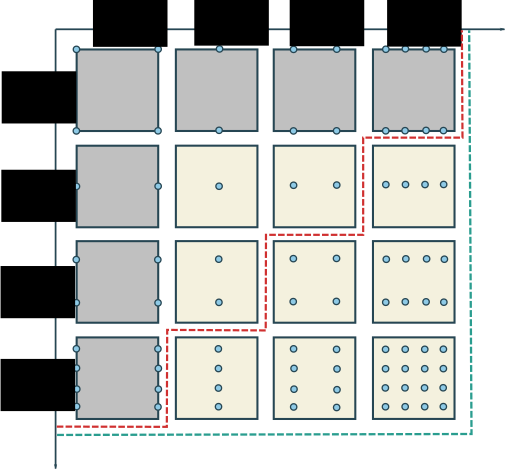
\includegraphics[width=.8\linewidth]{graphics/grid_subspaces}
  \subcaption{Hierarchical splitting of a grid point set}
\label{fig:grid_splitting}
    \end{minipage}%
    \begin{minipage}{0.28\textwidth}
        \centering
  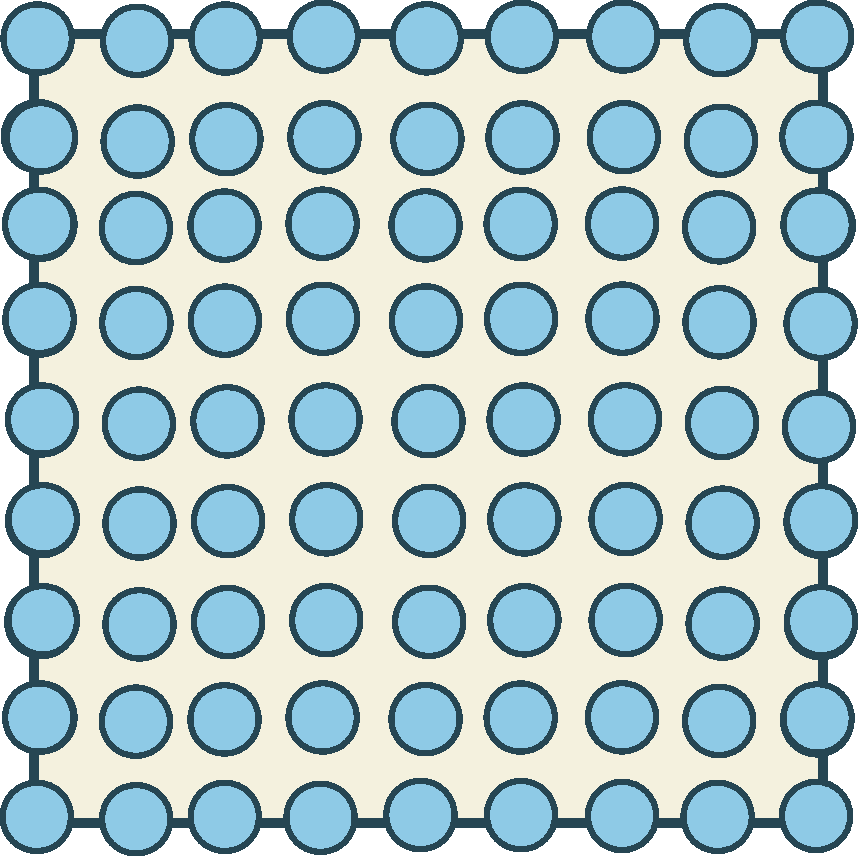
\includegraphics[width=.8\linewidth]{graphics/full_grid}
  \subcaption{Grid points of $V^{\text{fb}}_{3}$}
\vspace{4.5mm}
  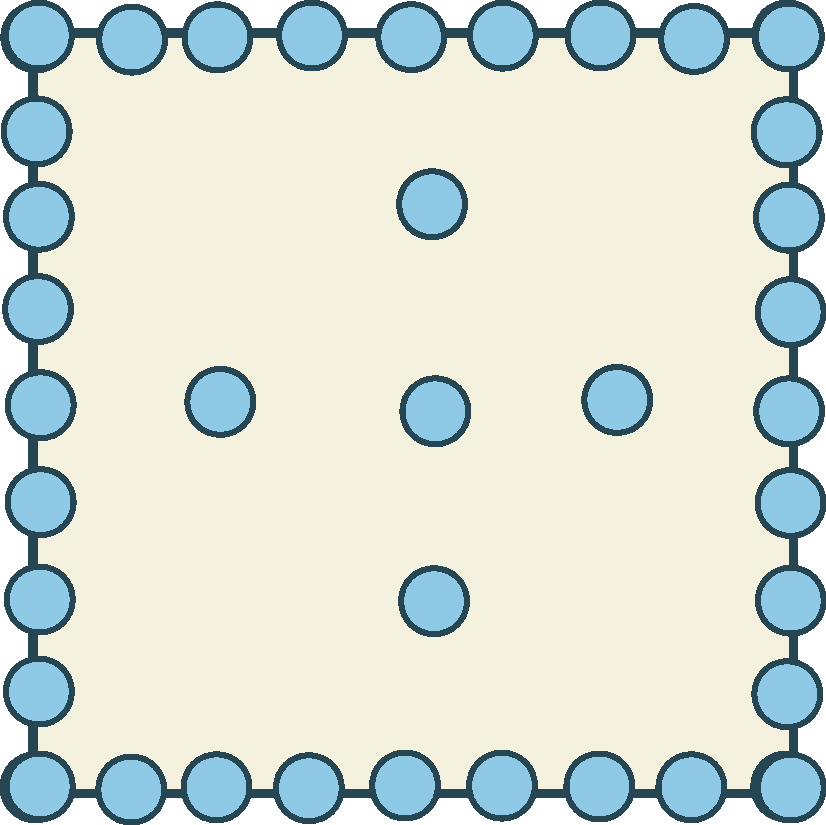
\includegraphics[width=.8\linewidth]{graphics/sparse_grid}
  \subcaption{Grid points of $V^{\text{sb}}_{3}$}
    \end{minipage}
\vspace{2.5mm}
\delimit
\caption{Construction of different grids from hierarchical grid point set increments. The full boundary grid $V^{\text{fb}}_{3}$ is a sum of all grid increments outlined in dotted \greencomma\,\,the sparse boundary grid $V^{\text{sb}}_{3}$ is a sum of all grid increments outlined in dotted \reddot\,\,Boundary grid point increments are shaded in \greydot}
\label{fig:grid_construction}
\end{figure}
\end{mdframed}

\section{Sparse grid surrogates}
\label{sec:gsc}

Sparse grid surrogates that try to approximate a model function can be constructed using multiple different approaches.
As sparse grid surrogate is a linear combination of all basis functions, to represent the instance $\hat{f}$, each basis function $\phi_{\underline{\ell},\underline{i}}$ is assigned a weight $\alpha_{\underline{\ell},\underline{i}}$, also called hierarchical surplus
.
\begin{definition}[Sparse grid surrogates]
Let $\phi_{\underline{\ell},\underline{i}}$ be multivariate basis functions and $X$ a set of grid points.
Furthermore, let $\alpha_{\underline{\ell},\underline{i}} \in \mathds{R}$ be the hierarchical surplusses.\\
A grid surrogate is then the linear combination
\begin{equation}
\hat{f}(x) \coloneqq \sum_{x_{\underline{\ell},\underline{i}} \in X} \alpha_{\underline{\ell},\underline{i}} ~ \phi_{
\underline{\ell},\underline{i}}(x).
\end{equation}
\end{definition}
%
In the case of a regular sparse grid with $X=X^{\mathrm{s}}_{\ell}$ for example, the surrogate instance can be expressed with
\begin{equation}
\hat{f}(x) = \sum_{|\underline{\ell}|_1 \leq \ell, \underline{1} \leq \ell'} \sum_{\underline{i} \in {H_{\underline{\ell}}}} \alpha_{\underline{\ell},\underline{i}} ~ \phi_{
\underline{\ell},\underline{i}}(x).
\end{equation}
%
The hierarchical surplusses can be computed with a variety of different methods, which results in multiple possible sparse grid construction schemes.
Most of the times, the interpolation approach to approximate model function is used.
In cases where only a function sample is given, a sparse grid surrogate can also be constructed through regression.

\paragraph{Interpolation}
The interpolation method is the most simple and common sparse grid surrogate construction scheme.
It evaluates the model function at every grid point and performs a hierarchization algorithm to obtain the hierarchical surplusses $\alpha_{\underline{\ell},\underline{i}}$.
The resulting surrogate constructed with the hierarchization method equals the model function at all grid points, such that $\forall x_{\underline{\ell},\underline{i}} \in X \colon f(x)=\hat{f}(x)$.
As the model function has to be evaluated at every grid point, a grid interpolation surrogate requires exactly $|X|$ function evaluations at the grid points and can not be used to approximate a function from a given function sample.

\paragraph{Regression}
An alternative surrogate construction scheme is sparse grid based regression \cite{Pflueger2010}.
In contrast to interpolation, a regression approach does no longer require the function values at the grid points to interpolate between them.
Instead, it uses established regression approaches to iteratively improve the weights $\alpha_{\underline{\ell},\underline{i}}$ with regards to the approximation error, by using train and validation samples drawn from the model function.
As a result, the size of the function sample, and therefore the amount of function evaluations, does no longer have to be equal to the amount of grid points.
This provides a greater level of flexibility, as the amount of model function evaluations and the amount of grid points can vary.

The basic approach is to solve the least squares problem for the function sample $S=\{(x_i, f(x_i)\}_{i=1}^n$ with the standard square loss function,
\begin{equation}
\varepsilon_{\text{MSE}}(\hat{f}) \coloneqq \frac{1}{n} \sum_{i=1}^n \left(f(x_i) - \hat{f}(x_i)\right)^2 ,
\end{equation}
and a regularization parameter $\lambda > 0$ to prevent overfitting.
Sparse grid based regression therefore tries to solve the regularized least squares problem to find the best possible surrogate for a set of possible smoothing factors $\lambda \in \Lambda$ and sparse grid level $\ell$ to obtain
\begin{equation}
\hat{f} = \argmin_{\hat{f} \in V^{\text{sb}}_{\ell}, ~ \lambda \in \Lambda} \varepsilon_{\text{MSE}}(\hat{f}) + \lambda R(\hat{f}).
\end{equation}


\section{Basis functions}

The multivariate basis functions $\phi_{\underline{\ell},\underline{i}}$, as defined in \cref{eq:basis_functions}, are a central aspect of sparse grids.
Many different families of basis functions exist, each with various levels of complexity, capabilities, and properties.
We will from now on refer to a family of basis functions of the same type as a basis.
In this section we will take a look at different elemtary basis functions used in this thesis and list reasons for using them.

\paragraph{Hat functions}
One of the most simple types of basis functions are hat functions.
A one-dimensional hat function $h(x) \coloneqq \max(1 - |x|,0)$ can be transformed into a basis function for a level $\ell$ and index $i$ with $\phi^h_{\ell,i}(x) \coloneqq h(2^\ell x-i)$.
They are also not differentiable at their supporting grid point $x_{\ell,i}$.

\paragraph{Modified basis functions}
One method of removing the need of using boundary grid points, at least to some degree, are modified basis functions.
These basis functions do not require grid points at the boundary and instead extrapolate the values at the boundaries from the grid points closest to the boundaries by using a modified version of normal basis functions.
It is possible to modify any non-boundary basis functions $\phi_{\ell,i}$ by defining the modified basis with
\begin{equation}
\phi^{\mathrm{mod}}_{\ell,i}(x) \coloneqq
\begin{cases}
1 &, \ell=1\\
\phi^{\mathrm{left}}_{\ell}(x)&, \ell>1, i=1\\
\phi^{\mathrm{right}}_{\ell}(x)&, \ell>1, i=2^\ell - 1\\
\phi_{\ell,i}(x)&, \text{else}
\end{cases},
\nonumber
\end{equation}
where $\phi^{\text{left}}_{\ell}$ and $\phi^{\text{right}}_{\ell}$ are special boundary extrapolation functions that are usually are similar with regards to their construction compared to the normal basis functions $\phi_{\ell,i}$.

\paragraph{Splines}
One solution to eliminating the hat basis discontinuities are B-Splines, which are just piecewise polynomials.
They can also be combined with the modified basis technique to obtain a modified B-Spline basis.

\begin{definition}[Fundamental property]
A family of univariate basis functions $\phi_{\ell,i}$ fulfills the fundamental property iff
\begin{equation}
\begin{split}
&\phi_{\ell,i}(x_{\ell', j}) = 0, ~~  \ell' < \ell, j \in H_{\underline{\ell'}},\\
&\phi_{\ell,i}(x_{\ell', j}) = \delta_{ij}, ~~  j \in H_{\underline{\ell'}}.
\end{split}
\nonumber
\end{equation}
As the used multivariate basis functions are constructed using the tensor-product approach, the fundemental property holds for a multivariate basis if it holds for the univariate one.
\end{definition}
%
A multivariate basis that fulfills the fundamental property can be hierarchized very efficiently through the unidirectional principle \cite{Balder1994} by applying a hierarchisation operator iteratively on every dimension separately, effectively breaking down the hierarchisation process into a series of one-dimensional hierarchisations.

\section{Spatially adaptive sparse grids}

In many cases, generating a regular sparse grid can be improved upon by introducing adaptivity into the process.
This allows us to spend more grid points, and therefore be more accurate, in regions that are more important and conversely reduce the amount of grid points spent in less important regions.
One method of implementing adaptivity during the sparse grid construction process are spatially adaptive sparse grids \cite{Pflueger2012}.
The central idea of them is to define a grid point hierarchy, such that each non-boundary grid point has two child grid points on the next level increment along every dimension.
A stepwise algorithm then add these child grid points to the surrogate if they are needed and do not exist yet.
This creation of new grid points that stem from a parent grid point is called the refinement of a grid point.

\begin{definition}[Hierarchical grid point children]
Let $x_{\underline{\ell},\underline{i}} \in X$ be a grid point.
We define
\begin{equation}
c_{k}^{\mathrm{left}}(x_{\underline{\ell},\underline{i}}) \coloneqq (x_{\ell_1,i_1}, \dots, x_{\ell_k + 1,2  i_k - 1} \dots, x_{\ell_d,i_d}), ~~ 
\end{equation}
as its left child if $i_k > 0$ along the $k$-th dimension and
\begin{equation}
c_{k}^{\mathrm{right}}(x_{\underline{\ell},\underline{i}}) \coloneqq (x_{\ell_1,i_1}, \dots, x_{\ell_k + 1,2  i_k + 1} \dots, x_{\ell_d,i_d}), ~~ 
\end{equation}
as its right child along the $k$-th dimension if $i_k < 2^{\ell_k}$.
In addition, we define
\begin{equation}
c_{k}(x_{\underline{\ell},\underline{i}}) \coloneqq
\begin{cases}
\left\{c_{k}^{\mathrm{right}}(x_{\underline{\ell},\underline{i}})\right\}&, i_k=0\\
\left\{c_{k}^{\mathrm{left}}(x_{\underline{\ell},\underline{i}})\right\}&,i_k= 2^{\ell_k}\\
\left\{c_{k}^{\mathrm{left}}(x_{\underline{\ell},\underline{i}}), ~ c_{k}^{\mathrm{right}}(x_{\underline{\ell},\underline{i}}) \right\}&, \text{else}
\end{cases}
\end{equation}
as the set of possible children of a grid point along dimension $k$, and 
\begin{equation}
c(x_{\underline{\ell},\underline{i}}) \coloneqq \bigcup_{k=1}^d \left\{c_{k}(x_{\underline{\ell},\underline{i}})\right\}
\end{equation}
as the set of children of a grid point.
It always holds that $\abs{c(x_{\underline{\ell},\underline{i}})} \leq 2d$, and in case there is no boundary involved, $\abs{c(x_{\underline{\ell},\underline{i}})}=2d$ also holds.\\
Furthermore, we define a grid point $x_{\underline{\ell},\underline{i}} \in X$ as a leaf grid point if it holds that
\begin{equation}
c(x_{\underline{\ell},\underline{i}}) \cap X = \emptyset,
\end{equation}
\ie no child grid points are already contained in $X$.
\end{definition}
%
To choose the best grid points to refine, a refinement criterion is introduced.
This abstract refinement criterion assigns a value to grid point such that the grid points with the highest value can be refined.
\begin{definition}[Refinement criterion]
Let $X$ be a set of grid points.
Then $\xi \colon X \mapsto \mathds{R}$ denotes the refinement criterion function, which assigns each grid point a value that determines the suitability of a refinement.\\
The commonly used surplus criterion
\begin{equation}
\xi_s(x_{\underline{\ell},\underline{i}}) \coloneqq \abs{\alpha_{\underline{\ell},\underline{i}}}
\end{equation}
just uses the absolute hierarchical surplus value, as a high value indicates steep rates of change in the area of a grid point.
\end{definition}
%
To prepare for an iterative adaptivity algorithm, we define the grid points of adaptive sparse grids after $m$ steps as $X_a^{(m)}$.
A spatially adaptive sparse grid usually starts out as a regular sparse grid with a coarse level, \ie $X_a^{(0)}=X^{\text{s}}_{\ell}$.
Then, during the $m$-th iteration, we first order all leaf grid points with
\begin{equation}
\xi(x_1) \geq \dots \geq \xi(x_p), ~~ x_1, \dots, x_p \in X_a^{(m-1)},
\end{equation}
and then perform $k$ refinements to obtain $X_a^{(m)}=X_a^{(m-1)} \cup c(x_1) \cup \dots \cup c(x_k)$.
Usually, if a leaf grid point is refined, all children are created because selective grid point creation would create additional overhead.
After $q$ steps, the spatially adaptive sparse grid with the grid points $X_a^{(q)}$ is finished.
The important parameters that influence the results are the iterations $q$, the refinements per step $k$, the refinement criterion $\xi$, as well as the initial grid type and size of $X_a^{(0)}$.

Various other established adaptivity methods exist, such as dimensionally adaptive sparse grids, which uses a more rigid refinement rule that adds all grid points of whole hierarchical subspaces to the surrogate.
Another more recent method are spatially dimension adaptive sparse grids \cite{Khakhutskyy2016}.
One small downside of spatially adaptive sparse grids is that all children grid points are added in a refinement step.
In a dimensionality reduction focused setting this behaviour is not optimal, since we want to focus on more important dimensions only when refining a grid point.
Spatially dimension adaptive sparse grids provide a solution by only selectively adding child grid points along a certain dimension.

\section{Radial basis functions}

Radial basis function interpolation \cite{Broomhead1988} is another technique for function interpolation that utilizes radial basis functions to construct a surrogate.
A radial basis function $\varphi' \colon \Omega \mapsto \mathds{R}$ is a function whose value solely depends on the distance between its input and its center point $c \in \Omega$, \ie it holds that $\varphi$ is a radial function of the form $\varphi'(x)=\varphi(\|x - c\|)$.
The univariate function $\varphi$ is then called the radial kernel centered at $c$.
Similar to sparse grid surrogates, a radial basis function surrogate is a linear combination,
\begin{equation}
f(x) \approx \sum_{i=1}^m \omega_i \varphi(\|x - c_i\|),
\end{equation}
of $m$ basis functions with center points $c_i$ and weights $\omega_i$.
In the context of this thesis, only Gaussian functions with the Euclidean distance $|\cdot |_2$ measure are used as basis functions.
Gaussian basis functions have the form
\begin{equation}
\varphi(x) \coloneqq e^{-(\epsilon |x - c_i|_2)^2}.
\end{equation}
%
The only parameter that can be tuned is $\epsilon$, which is referred to as the shape parameter and is used to scale the effects of the input radius.
Given a set of center points, type of basis functions, and shape parameter $\epsilon$, we can calculate the weight coefficients $\omega_i$, usually by using a linear least squares technique.
This, combined with the fact that exponentially more center points are needed to maintain the same level coverage when model dimensions increase, also causes this method to suffer from the curse of dimensionality.

Radial basis function approximation is covered in this thesis, as it is almost a polar opposite to the grid based approximation methods.
Radial basis function surrogates allow arbitrary center points, while sparse grid surrogates require a strict, hierarchical, and axis-aligned grid.
Furthermore, radial basis functions are fundamentally different to tensor-product based basis functions with regards to their orientation.
While tensor product basis functions are strictly axis-aligned, radial basis functions are unaware of the concept of axis-alignment or orientation.
This property will allow us to use radial basis functions as a reference when investigating the effects of basis function alignment later on.

\section{Sampling}
\label{sec:lds}

In the coming chapters we will often make use of some Monte-Carlo based methods that require function samples from the model function.
For this purpose, even the relatively simple process of drawing samples from the model input parameter probality distribution can improved in different ways to achieve better results.
We assume that the inputs of model functions are distributed according to a multivariate distribution
\begin{equation}
\rho(x)=\prod_{i=1}^d \rho_i(x_i),
\end{equation}
which is made up out of $d$ independent distributions $\rho_i$.

A problem that arises when generating a sequence of random samples using a pseudorandom number generator to draw samples from the uniform input distribution $\rho=\mathcal{U}[0,1]^d$ is that the sequence does not cover the function domain as evenly and quickly as it theoretically can.
One solution are so-called low-discrepancy sequences, also called quasirandom sequences to distinguish them from normal pseudorandom sequencens.
These sequences are more evenly distributed than pseudorandom samples and therefore have a lower discrepancy.
Thus, they cause the result of various Monte-Carlo methods to converge faster than it would if we were just using the same amount of pseudorandom samples.
A commonly used quasirandom sequence is the Sobol sequence \cite{Niederreiter1988}, which is also used in this thesis.
It is generated using the Antonov and Saleev variant, which uses the Gray code of $i$ to construct the $i$-th sample.

This approach can also be extended to allow for the generation of pseudorandom samples from non-uniform distributions through the commonly used inverse transform sampling method \cite{Devroye1986}.
However, this approach is not used in this thesis, as the gains are minimal.

\section{Error metrics}
\label{sec:errors}

To evaluate the quality of a constructed surrogate $\hat{f}$, we define a couple of error metrics to measure the approximation error and also make it comparable to other surrogates.
An established and commonly used error metric for function approximation is the $L^2$ error:
\begin{definition}[$L^2$ error]
Let
\begin{equation}
||g||_{L^p}^p \coloneqq \int_{\Omega} \abs{g(x)}^p \mathrm{d}x
\end{equation}
be the $L^p$ norm for real functions $g \colon \Omega \mapsto \mathds{R}$.
We then define
\begin{equation}
\varepsilon_{\text{$L^2$}}(\hat{f}) \coloneqq \|f - \hat{f}\|_{L^2}=\sqrt{\int_{\Omega} |f(x) - \hat{f}(x)|^2 \mathrm{d}x}
\end{equation}
as the $L^2$ surrogate approximation error.
\label{def:l2}
\end{definition}
%
In numerics, to evaluate the accuracy of an estimator, the mean squared error and the root mean squared error are commonly used.
They can be described as the expected value of the squared errors and the square root of the expected value of the squared errors:
\begin{definition}[Mean squared error]
Let $\hat{f}$ be the surrogate for the model function and $S=\left\{(x_i, f(x_i)\right\}_{i=1}^n \subseteq \Omega \times \mathds{R}$ a set of samples.
We then define
\begin{equation}
\varepsilon_{\mathrm{MSE}}(\hat{f}) \coloneqq \frac{1}{n} \sum_{i=1}^n \left(f(x_i) - \hat{f}(x_i)\right)^2
\end{equation}
as the mean squared error for the surrogate based on the given sample.
In the same fashion, we also define
\begin{equation}
\varepsilon_{\mathrm{RMSE}}(\hat{f}) \coloneqq \sqrt{\varepsilon_{\mathrm{MSE}}(\hat{f})} = \sqrt{\frac{1}{n} \sum_{i=1}^n \left(f(x_i) - \hat{f}(x_i)\right)^2}
\end{equation}
as the root mean squared error.
\end{definition}
%
The RMSE is closely related to the definition of the continous $L^2$ error, as it is just a discrete version of it.
It holds that $\lim_{n \to \infty} \varepsilon_{\mathrm{RMSE}}(\hat{f}) = \varepsilon_{\text{$L^2$}}(\hat{f})$.

One problem of the introduced error metrics is that they are all sensitive to the size of the function values.
To improve upon these absolute error metrics and allow for comparisions across model functions with different ranges of function values, we define normalized errors:
\begin{definition}[Normalized root mean squared error]
Let $\hat{f}$ be the surrogate for the model function $f$ and $S=\{(x_i, f(x_i)\}_{i=1}^n \subseteq \Omega \times \mathds{R}$ a set of samples.
We then define
\begin{equation}
\varepsilon_{\mathrm{NRMSE}}(\hat{f}) \coloneqq \frac{\varepsilon_{\mathrm{RMSE}}(\hat{f})}{\max_{x \in S} f(x) - \min_{x \in S} f(x)}
\end{equation}
as the normalized root mean squared error.
\end{definition}


\chapter{Input transformations}
\label{chap:c3}

A lot of work has already gone into exploring all kinds of variants and optimizations for sparse grids, which resulted in many different families of basis functions and grid types \cite{Valentin2019, Feuersaenger2010}.
Moreover, many algorithms that work on sparse grids \cite{Gerstner1998, Garcke2001, Pflueger2010, Valentin2019, Rehme2021} have also been developed, such that the general sparse grids technique can be applied in a better and more flexible way to many different kinds of problems.
In the related sparse grid literature, the process of optimizing sparse grids itself was the primary focus most of the time.
In contrast to this approach, we instead inspect and adapt the inputs itself before they are passed to sparse grid based methods.
The basic idea that is propagated in this thesis is that, instead of directly using the sparse grids to approximate a function with $f(x) \approx \hat{f}(x)$, we insert another layer of flexibility into the process by introducing an input transformation function $t$ and creating the surrogate $\hat{f}$ in tandem with $t$, such that a transformed sparse grid approximation $f(x) \approx \hat{f}(t(x))$ performs better.
This general idea and also the necessary details will be expanded upon in this chapter.

\section{Intrinsic dimensionality}
\label{sec:intrinsic}

There already exist several techniques used in signal processing and data science that are related to the idea of input transformations, for example principal component analysis \cite{Abdi2010}, which tries to find and exploit certain characteristics of the input data.
Related to PCA is the concept is intrinsic dimensionality \cite{Bennett1969}.
The intrinsic dimensionality of a function or dataset is the minimal amount of features required to completely represent its output.
It can be used as a guidance to determine a lower bound on the dimensionality of the model function and also optionally exploit the knowledge to construct a lower-dimensional surrogate and thus perform a dimensionality reduction.

\begin{definition}[Intrinsic dimensionality]
A $d$-dimensional function $f(x_1, \dots, x_d)$ has an intrinsic dimensionality of $r \leq d$, if there exists a transformation function $t \colon \Omega \mapsto \Omega_r$, such that
\begin{equation}
\forall x \in \Omega \colon f(x)=f_t(t(x)).
\end{equation}
\label{def:intrinsic}
Even though we do not explicitly define $\Omega_r$, it too should be a bounded Euclidian product such that it can  transformed into the unit hypercube $\Omega_r=[0,1]^r$, similar to $\Omega$.
\end{definition}
%
We define the minimal intrinsic dimensionality of a function as the optimal intrinsic dimensionality $r^\ast$.
However, even if we are able to find a non-optimal $r$-dimensional transformation with $r > r^\ast$ that satisfies the requirement of \cref{def:intrinsic}, we still have gained an advantage and can define that function as having an intrinsic dimensionality of at most $r$.
Even if it holds that $r=r^\ast$, we still define it as having an intrinsic dimensionality of at most $r$, since in many cases we don't know the actual intrinsic dimensionality $r^\ast$ without a proof.

Since we are dealing with function approximation problems in this thesis, we extend definition \cref{def:intrinsic} to also allow for approximation errors:
\begin{definition}[Approximate intrinsic dimensionality]
Let $f$ be $d$-dimensional function, $\varepsilon$ an error metric from \cref{sec:errors}.
We then define $f$ as having an approximate intrinsic dimensionality of $r \leq d$ with an error of $e$, if there exists a function $t \colon \Omega \mapsto \Omega_r$, such that
\begin{equation}
e=\varepsilon\left(f(x) - f_t(t(x))\right).
\end{equation}
\end{definition}
%
Similar to the minimal intrinsic dimensionality $r^\ast$, we are not concerned about the finding, and also usually do not know, the minimal error $e^\ast= \argmin_{t, f_t} \varepsilon(f(x) - f_t(t(x)))$ for a given $r$.
With the introduction of approximation errors into the intrinsic dimensionality definition, there is also room to determine a good tradeoff between intrinsic dimensionality and approximation error.
The main goal of making use of lower dimensional function surrogate is then accomplished by finding functions $t$ and $f_t$ that provide a good tradeoff between dimensionality and approximation error.

To achieve a good convergence rate and general representativeness of a drawn set of samples, \eg for a quadrature operation, it is vital to achieve low-discrepancy and cover the input space $\Omega$ more evenly.
Under normal circumstances, to achieve the same discrepancy in a high-dimensional space as in a low-dimensional space,
exponentially more samples are required.
However, combining this requirement with the concept of intrinsic dimensionality, we observe that we effectively only need to cover $\Omega_r$ and adapt any operation that normally works on $\hat{f}$ to instead work on the lower dimensional surrogate $\hat{f_t}$.
The main advantage is that the lower amount of samples required to achieve a good coverage of the definition space of $f_t$ would depend on $r$ and not on $d$.

\begin{definition}[Transformed distribution]
Let $t^{-1}(x_{t})=\{x \in \Omega \mid t(x)=x_{t}\}$ be the inverse transformation function.
We then define the transformed distribution,
\begin{equation}
\rho_t \colon \Omega_r \to \mathds{R_+}, ~~ \rho_t(x_t)=\int_{t^{-1}(x_t)} \rho(x) \; \mathrm{d}x.
\end{equation}
This is also a valid probability distribution since it holds that
\begin{equation}
\int_{\Omega_t} \rho_t(x_t) \; \mathrm{d}x=\int_{x_t \in \Omega_r} \int_{t^{-1}(x_t)} \rho(x) \; \mathrm{d}x = \int_{\Omega} \rho(x) \; \mathrm{d}x = 1.
\end{equation}
\end{definition}
%
As a result, applying a transformation has on the original input distribution has the potential to change the distribution type.
For example, a uniform distribution $\rho=\mathcal{U}[0,1]^d$ could be transformed into a non-uniform distribution $\rho_t$.
Furthermore, the quality and properties of transformed low discrepancy sequences (\cref{sec:lds}) changes compared to its original, untransformed sequence \cite{Wang2008}.
To effectively sample from $\rho_t$, it is still easier to just draw the samples $(x_1, \dots, x_n)$ from $\rho$ directly and feed them into the transformation function to obtain the transformed sequence $(t(x_1), \dots, t(x_n))$, which is distributed according to $\rho_t$.

\section{Limitations of sparse grids}

All grid-based interpolation methods share the common problem of being affected by the curse of dimensionality \cite{Bellman1961} to some degree.
This means that as the model dimensionality grows, the amount of grid points and the model function evaluations required to generate a sparse grid grow too fast and put a limit on how many dimensions are feasible.
Sparse grids itself are already a pretty effective strategy to reduce the consequences of the curse of dimensionality compared to full grids, as they provide a good tradeoff between the amount of grid points used and the interpolation accuracy, but they can only weaken and delay the effects of the curse of dimensionality.
Therefore, in higher dimensions, employing some form of dimensionality reduction is necessary.
Of course, the effectiveness of dimensionality reduction techniques are limited by the minimum amount of accuracy that is required for the specific use case.
In this section we take a look at a few already established approaches to sparse grid based dimensionality reduction and look at their properties with the help of simple example model functions.

The first example model function,
\begin{equation}
f_1(x_1, x_2)=\sin(2 \pi x_1) + 1,
\end{equation}
 is designed to be a good fit for grid based methods.
It is a two-dimensional function, where only the first component and a constant term contribute to the total function value, while the second component does not.
One can easily see that it has an intrinsic dimensionality of $1$ according to \cref{def:intrinsic}, since a transformation function could just cut off the second input component.
However, by simply rotating the function by a few degrees, we obtain the second example model function,
\begin{equation}
f_2(x_1,x_2)=\sin(2 \pi x_1') + 1, ~~~~~ x_1'=\cos(0.15 \pi) x_1 -\sin(0.15 \pi) x_2,
\end{equation}
which is also a two-dimensional function but importantly still has an intrinsic dimensionality of $1$.

\subsection{Spatially adaptive sparse grids}

Both functions can be approximated using spatially adaptive sparse grids.
We can then investigate how their generated grid points and interpolation errors compare.

\begin{mdframed}[style=style]
\begin{figure}[H]
\begin{subfigure}{.5\textwidth}
  \centering
  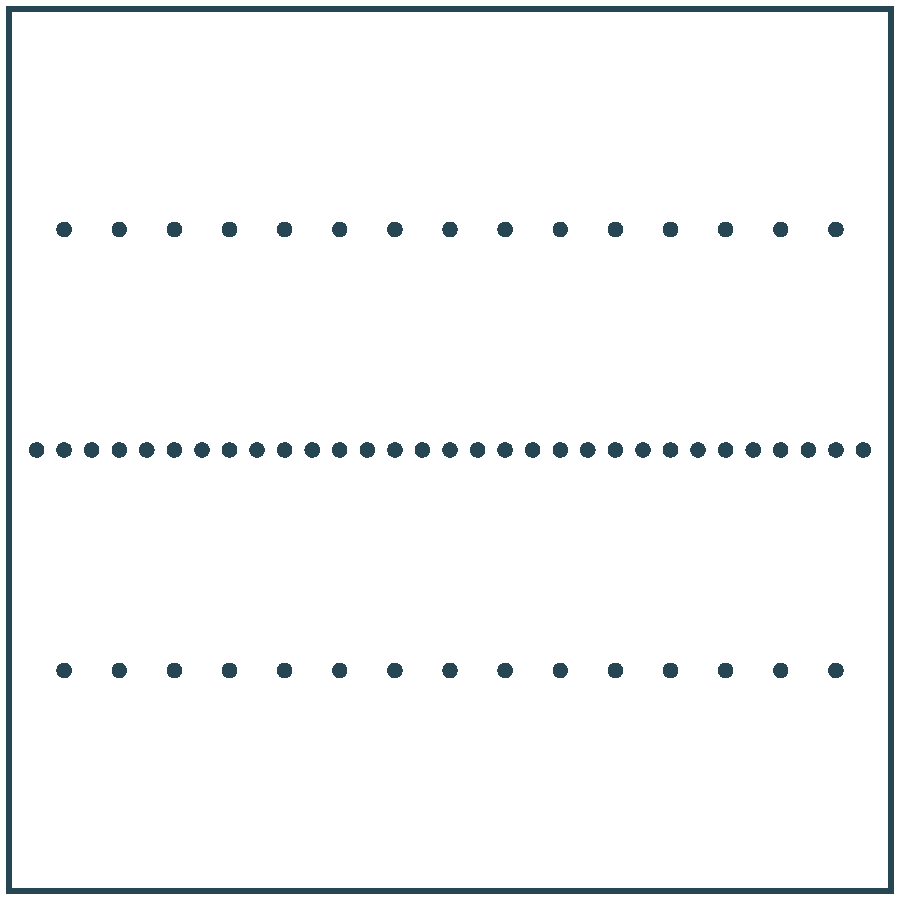
\includegraphics[width=.65\linewidth]{graphics/grid_f1}
  \captionof{figure}{Grid points for $f_1$}
  \label{fig:grid_f1}
\vspace{2.5mm}
\end{subfigure}%
\begin{subfigure}{.5\textwidth}
  \centering
  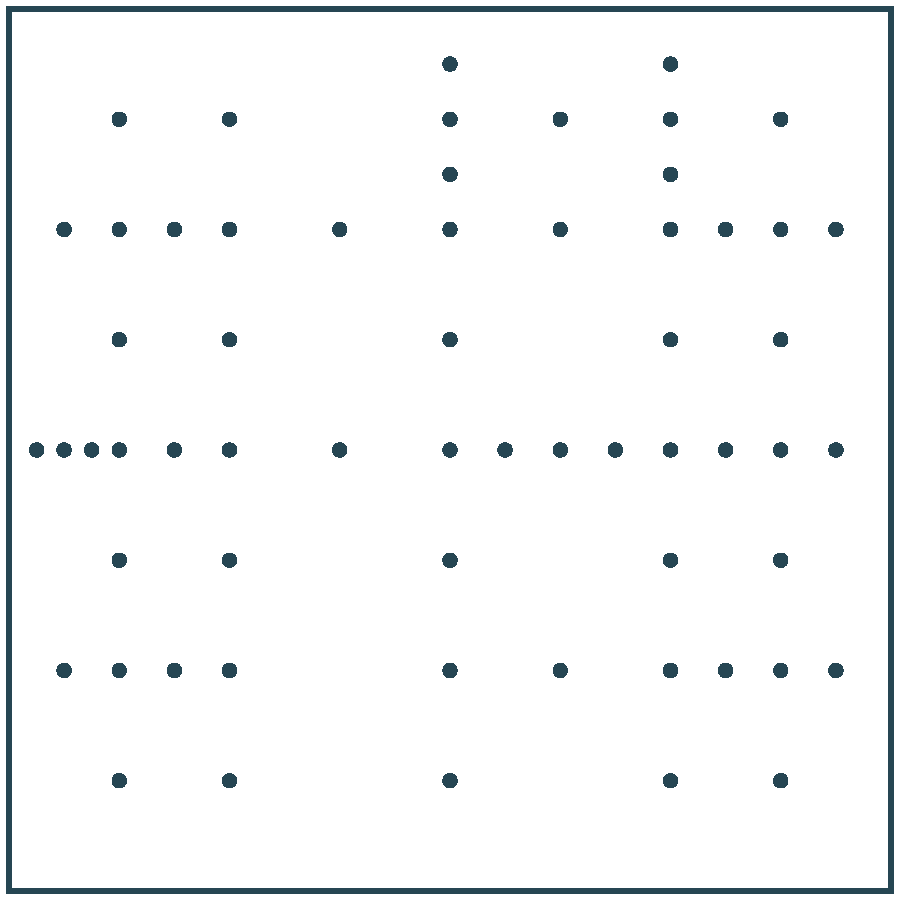
\includegraphics[width=.65\linewidth]{graphics/grid_f2}
  \captionof{figure}{Grid points for $f_2$}
  \label{fig:grid_f2}
\vspace{2.5mm}
\end{subfigure}
\delimit
\captionof{figure}{Grid points of generated spatially adaptive sparse grids for $f_1$ and $f_2$ that started out as a regular sparse grid with level $\ell=1$. The surplus refinement criterion, 15 refinements steps with one grid point refinement per step, and modified linear basis functions were used.}
\label{fig:grids}
\end{figure}
\end{mdframed}
%
\Cref{fig:grids} shows how spatially adaptive sparse grids are affected by the different alignment of function terms.
The spatially adaptive strategy is able to exploit the one-dimensional nature of $f_1$ by only refining along the first dimension and therefore spending the grid points only where they matter.
However, the intrinsically one dimensional term of $f_2$ can not be exploited, as it is no longer axis-aligned.
This can be deduced from the fact that grid points all over the grid and along both dimensions are refined.
Note that due to the default refinement rule that add all child grid points, the upper and lower grid point rows in \cref{fig:grid_f1} are created even though they are not necessary.
A tweaked refinement rule could easily fix this however.
This observation is reinforced by the actual approximation errors of surrogates for both functions seen in \cref{fig:grid_approx_f2}.

\subsection{Radial basis functions}

Radial basis functions behave differently than sparse grids when being applied to the same two functions, as their basis functions are not constructed using the tensor-product approach.
Instead they are orientation agnostic, as only the radius relative to a support point determines the basis function value.
Therefore, as seen in \cref{fig:grid_approx_f1}, the approximation errors stay pretty much identical in both cases.
However, the approximation error for $f_1$ is worse than the sparse grid surrogate error, as radial basis functions are not suited for approximating functions with a constant dimension when being compared to modified basis functions, which come with a constant component well suited for that.

\begin{mdframed}[style=style]
\begin{figure}[H]
\begin{subfigure}{.5\textwidth}
  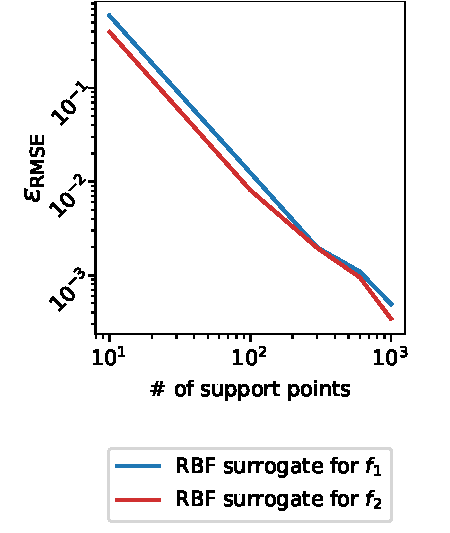
\includegraphics[width=\linewidth]{graphics/grid_approx_f1}
  \subcaption{RBF surrogates created with Gaussian basis functions, Euclidean distance measure, and shape parameter $\epsilon=0.5$.}
  \label{fig:grid_approx_f1}
\vspace{2.5mm}
\end{subfigure}%
\begin{subfigure}{.5\textwidth}
  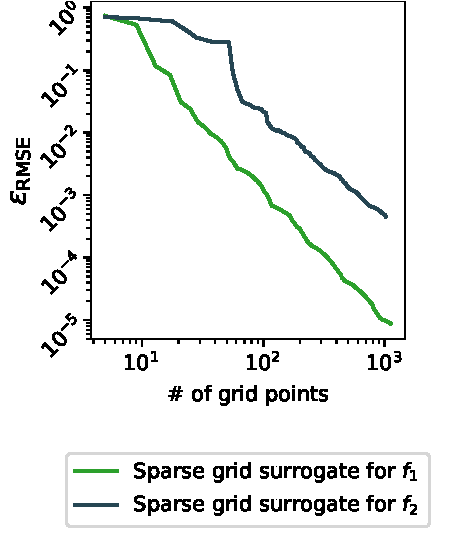
\includegraphics[width=\linewidth]{graphics/grid_approx_f2}
  \subcaption{Spatially adaptive sparse grids with $\ell=1$, surplus refinement criterion, 280 single refinement steps, and mod. linear basis functions.}
  \label{fig:grid_approx_f2}
\vspace{2.5mm}
\end{subfigure}
  \delimit
\caption{
Approximation error comparision for both example functions $f_1$ and $f_2$ using spatially adaptive sparse grids and radial basis functions.}
  \label{fig:dim_reduction_errors}
\end{figure}
\end{mdframed}

\subsection{Variance-based sensitivity analysis}

The method of variance-based sensitivity analysis, a form of global sensitivity analysis introduced by Sobol \cite{S01},  is a well established method in statistics to determine the importance of model input parameters.
Given a set of dimension indices $D=\{1,\dots,d\}$, we define the set of ANOVA-components $C \coloneqq \mathcal{P}(D)$, where an ANOVA-component $c \in C$ that contains a specific dimension index $i \in D$ indicates that a function term is varying along the $i$-th dimension.
We can then decompose a model function into the componentwise sum,
\begin{equation}
f(x)=\sum_{c \in \mathcal{P}(D)} f_{c}(x),
\label{anovaComp}
\end{equation}
also called the ANOVA decomposition of $f$.

A decomposition of a high dimensional function $f$ into $|\mathcal{P}(D)|=2^d$ lower dimensional function terms allows for an examination of individual terms with the goal identifying terms that contribute the least amount of variance to the total function variance.
This decomposition can also be employed on sparse grids \cite{F10} by using special semi-orthogonal basis functions, for example a wavelet basis, to represent the $f_c$.
Since the terms $f_i$ are required to be semi-orthogonal, we can define a variance function,
\begin{equation}
\sigma^2(f) \coloneqq \int_{\Omega} f(x)^2 \rho(x) ~ \text{d} x=\sum_{c \in \mathcal{P}(D)} \sigma^2(f_c),
\end{equation}
in an additive manner.
For every ANOVA component $c \in C$, we can then calculate the variance share, also called Sobol index,
\begin{equation}
S_{c} \coloneqq \frac{\sigma^2(f_{\underline{c}} )}{\sigma^2(f)}, ~~ \sum_{c \in \mathcal{P}(D)} S_{c} = 1.
\end{equation}
Computing the Sobol indices of all terms for both example functions gives insight into the structure of the function and tells us what share of the function we are able to represent with axis-aligned terms of varying dimension.
It helps us to understand, why spatial adaptivity succeeds only for one of them.

\begin{mdframed}[style=style]
\begin{figure}[H]
        \centering
\begin{minipage}[H]{.45\textwidth}
  \centering
  \begin{tabular}{ l c c }
\hline \hline
& $2 \notin c~$ & $2 \in c$ \\
\hline
$1 \notin c$ & 0.667 & 0.0\\
$1 \in c$ & 0.333 & 0.0\\
\end{tabular}
\delimit
  \captionof{table}{Sobol indices of all ANOVA components for $f_1$.}
  \label{tab:anova_f1}
    \end{minipage}%
    \hspace{.05\textwidth}
    \begin{minipage}[H]{0.45\textwidth}
  \centering
  \begin{tabular}{ l c c }
\hline \hline
& $2 \notin c~$ & $2 \in c$ \\
\hline
$1 \notin c$ & 0.636 & 0.001\\
$1 \in c$ & 0.163 & 0.199\\
\end{tabular}
\delimit
  \captionof{table}{Sobol indices of all ANOVA components for $f_2$.}
  \label{tab:anova_f2}
    \end{minipage}
\end{figure}
\end{mdframed}
%
The ANOVA method decomposes the two-dimensional functions into four terms.
A constant term $f_\emptyset$, two one-dimensional terms $f_{\{1\}}$ and $f_{\{2\}}$, and a two dimensional term $f_{\{1,2\}}$.

As we can see in \cref{tab:anova_f1}, at least for the function $f_1$, the method correctly identifies that only the terms $f_\emptyset$ and $f_{\{1\}}$ have some output variance with $\sigma^2(f_\emptyset)=? > 0.667$ and $\sigma^2(f_{\{1\}})=? > 0.333$.
Therefore, the other terms can be dropped and the function can be completely represented using only one-dimensional function terms.

However, we can see in \cref{tab:anova_f2} that the ANOVA method attributes a share of output variance to all terms, since for all ANOVA components it holds that $\sigma^2(f_{c}) > 0.199$.
In this case, the ANOVA method shows us that no dimensionality reduction can be applied, as the term $f_{\{1,2\}}$ has some variance contribution.
Note that if the constant term $f_\emptyset$ is excluded from the analysis, as is often done, the effects of the changed alignment of $f_2$ on the Sobol indices would be even greater.

\subsection{Summary}

To summarize, we saw that a fundamental property of any approximation method that uses basis functions created by using the tensor product approach is that the approximation quality depends on whether the model function primarily also consists out of axis-aligned terms or not.
In contrast to this behaviour, other basis functions, \eg radial basis functions, do not depend on the alignment of the function terms they are trying to approximate, \ie they can be seen as orientation agnostic.
In turn this means that an effective dimension reduction with conventional sparse grid based methods is highly dependent on the alignment of the model function.
Without adding another layer of flexibility, sparse grids can not use their full potential in many cases, as we have seen the with model function $f_2$.

\section{Linear hypercube transformations}

As the concept of intrinsic dimensionality allows us, at least in theory, to use arbitrary transformation functions to map into the lower-dimensional input space $\Omega_r$, there are many possible general types of transformation functions to choose from.
The previous chapter showed how a simple change of basis of the input parameters, \ie an orthogonal transformation of them, can have a huge impact on constructed sparse grid surrogates.

Motivated by this insight, the main approach that will be used and investigated in this thesis starts out with finding an orthonormal matrix $W \in \mathds{R}^{d \times d}$ that is aligned along the active directions of the model function in the best possible way.
This matrix $W$ is referred to as the active direction matrix, as the column vectors $w_i$ point into directions in which the function output has a high rate of change and are ordered by the level of change.
It should hold that $w_1$ is the most active direction, while $w_d$ is the most inactive direction.
Since all column vectors $w_i$ have to be orthogonal, they can not point into arbitrary directions and are limited by other active directions.
The concept of active directions and also ways of computing suitable active directions will be covered in the next section about active subspaces.

We then go one step further and also try to eliminate the most inactive directions of $W$, effectively performing a dimension reduction.
After performing a change of basis with $W$ on the inputs to obtain $W^T x$, we effectively eliminate the most inactive dimensions, as inactive directions are now mapped to inactive dimensions.
This results in the possibility of drastically reducing the amount of grid points while only suffering a small increase in error in theory, as only the most unimportant dimensions, which should not contribute a lot to the approximation error, are eliminated.

\begin{definition}[Transformation matrix]
Let $W \in \mathds{R}^{d \times d}$ be the active direction matrix with $W^T W=I$, and let $r \leq d$ be the reduced dimension.
We then define
\begin{equation}
W_r \coloneqq \begin{bmatrix}
  \\
    w_1 ~ w_2 ~ \dots ~ w_{r-1} ~ w_r\\
    \\
  \end{bmatrix}
\end{equation}
as the transformation matrix.
\end{definition}
%
As we can see, the transformation matrix is simply obtained from a given active direction matrix $W$ and a reduced dimension $r$ by cutting off the last $d - r$ directions from $W$.
For now, we assume that the $W$ and $r$ are given, but we will cover the process of determining those essential inputs later on in detail.
In case no vectors $w_i$ of $W$ are cut off, we call it an orientation changing linear transformation.
Otherwise, if $r < d$ and some vectors are cut off, we call it a dimensionality reducing linear transformation or just reducing linear transformation.

\subsection{Unit hypercube projections}

To construct a transformation function $t$ that maps from the $d$-dimensional unit hypercube $\Omega=[0,1]^d$ to the $r$-dimensional unit hypercube $\Omega_r=[0,1]^r$ with $r < d$ for a given transformation matrix $W_r$, several adjustments have to be made in order to obtain a usable transformation function as the naive approach with $W_r^T x$ would map inputs outside of $\Omega_r$ in certain cases.
When applying a linear transformation $W_r^T x$ on the elements of a hypercube $x \in \Omega$, the result can be described with the help of zonotopes:

\begin{definition}[Zonotope]
Let $m$ be the dimension of the zonotope, and let $k \geq  m$ be the amount of zonotope generators.
An $m$-dimensional zonotope
\begin{equation}
Z \coloneqq \left\{\sum_{i=1}^k g_i x_i \mid ~ -1 \leq x_i \leq 1\right\}
  \label{zonotope}
\end{equation}
with $k$ generator vectors $g_1, \dots g_k \in \mathds{R}^m$ corresponds a the $k$-dimensional minkowski sum.
\end{definition}


\begin{mdframed}[style=style]
        \centering
\begin{minipage}{.45\textwidth}
        \centering
  \captionof{figure}{Exemplary creation of a Zonotope $Z$ with $l=2$, $k=3$, and three generators $g_1,g_2,g_3$.\\
  The three generator vectors are drawn to the left and the zonotope $Z$ is drawn in \darkblue to the right with the origin being in \red.}
  \label{fig:zonotope}
    \end{minipage}%
    \begin{minipage}{0.55\textwidth}
        \centering
        \vspace{3.5mm}
  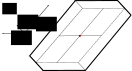
\includegraphics[width=0.8\linewidth]{graphics/zonotope}
  \hspace{-5.5mm}
    \end{minipage}
\end{mdframed}


When applying the projection $W_r^T$ to the inputs $x \in \Omega$, we can observe that
\begin{equation}
\begin{split}
W_r^T x=~W_r^T \sum_{i=1}^d x_i e_i=~\sum_{i=1}^d x_i p_i , ~~~~ p_i=W_r^T e_i,
\nonumber
\end{split}
\end{equation}
where the $p_i$ are just the projected unit vectors.
Therefore, since for all components are in the unit interval with $x_i \in [0,1]$, we can express the transformed inputs with
\begin{equation}
\{W_r^T x \mid x \in \Omega\}=\left\{\sum_{i=1}^d x_i p_i \mid x \in \Omega \right\}=\left\{ \sum_{i=1}^r x_i p_i \mid 0 \leq x_i \leq 1\right\}.
\label{wtx}
\end{equation}
To get \cref{wtx} closer to the zonotope definition in \cref{zonotope}, we first center the inputs $x \in \Omega$ before applying the projection and divide the generators $p_i$ by 2.
For this, let $c_i=(\frac{1}{2}, \dots, \frac{1}{2})^T\in \mathbb{R}^i$ be the center of the $i$-dimensional unit hypercube.
We can express this with
\begin{equation}
\begin{alignedat}{2}
&\left\{W_r^T (x - c_d) \mid x \in \Omega\right\}&&=\left\{W_r^T \sum_{i=1}^d \left(x_i - \frac{1}{2}\right) e_i \mid x \in \Omega \right\}\\
=&\left\{\sum_{i=1}^d \left(x_i - \frac{1}{2}\right) W_r^T e_i \mid x \in \Omega \right\}&&=\left\{\sum_{i=1}^d \left(x_i - \frac{1}{2}\right) w_i \mid x \in \Omega \right\}, ~~ w_i=W_r^T e_i\\
=&\left\{\sum_{i=1}^d \left(x_i - \frac{1}{2}\right) w_i \mid 0 \leq x_i \leq 1 \right\}&&=\left\{\sum_{i=1}^d x_i w_i \mid -\frac{1}{2} \leq x_i \leq \frac{1}{2} \right\}\\
=&\left\{\sum_{i=1}^d \frac{1}{2} x_i w_i \mid -1 \leq x_i \leq 1 \right\}&&=\left\{\sum_{i=1}^d x_i p_i \mid -1 \leq x_i \leq 1 \right\}, ~~ p_i=\frac{1}{2} w_i
\label{zonotope_form}
\end{alignedat}
\end{equation}

Therefore, defining the projection function with
\begin{equation}
p \colon \Omega \mapsto Z, ~~ p(x)=W_r^T (x-c_d)
\nonumber
\end{equation}
results in a projected input space that has the zonotope form of \cref{zonotope} with the $p_i$ are generators.
The projected zonotope is then
\begin{equation}
Z_{p} \coloneqq \left\{\sum_{i=1}^r p_i x_i , ~ -1 \leq x_i \leq 1\right\}, ~~ p_i \coloneqq \frac{1}{2} W_r^T e_i,
\nonumber
\end{equation}
where according to \cref{zonotope_form}, the projected input space is exactly the zonotope with $Z_{p}=p(\Omega)$.

\subsection{Surrogate space}

However, since the surrogate creation process expects inputs from a hypercube and not a zonotope, the zonotope $Z_p$ is first encased in an $r$-dimensional hypercube called the surrogate space $S$.
The surrogate space is then later scaled and aligned to obtain the unit hypercube $\Omega_r$.
Generators $q_1, \dots, q_r$ of the encasing hypercube can be calculated by applying the Gram–Schmidt process on the ordered zonotope genrators $p_i$ to obtain the orthogonal vectors
\begin{equation}
q_i \coloneqq \frac{q_i'}{\| q_i' \|},~~ q_i' \coloneqq p_i - \sum_{k=1}^{i-1} \frac{\langle p_k q_k'\rangle}{\langle q_k', q_k' \rangle} q_k'.
\label{q}
\end{equation}
The surrogate space $S$, which encases the zonotope $Z$, is then an $r$-dimensional hypercube with
\begin{equation}
S \coloneqq \left\{\sum_{i=1}^r s_i q_i x_i, ~ -1 \leq x_i \leq 1\right\},~~ s_i \coloneqq \sum_{k=1}^d \langle q_i, p_k\rangle.
\label{surrogate_space}
\end{equation}
where the scaling factors $s_i$ are chosen in such a way that the hypercube $S$ exactly matches the extent of the zonotope $Z_p$, as seen in \cref{fig:surrogate_space}.
The scaling 


\begin{mdframed}[style=style]
        \centering
\begin{minipage}{.49\textwidth}
        \centering
  \captionof{figure}{Construction of the encasing surrogate space $S$ for the zonotope $Z_p$ of \cref{fig:zonotope} according to \cref{surrogate_space}.\\
  The projected zonotope $Z_p$ is drawn in \lightblue, the encasing surrogate space $S$ in dotted \darkblue, and the origin in \red.}
  \label{fig:surrogate_space}
    \end{minipage}%
    \begin{minipage}{0.49\textwidth}
        \centering
        \vspace{3.5mm}
  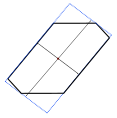
\includegraphics[width=0.8\linewidth]{graphics/surrogate_space}
  \hspace{-5.5mm}
    \end{minipage}
\end{mdframed}

As we only need $r$ generators for the surrogate space, but have $d$ generators of $Z_p$ available, not all $p_i$ are used in the surrogate space construction.
In theory, the generators $p_i$ that are used to calculate the $q_i$ are not ordered by default and also don't have to be ordered.
However, to emphasize the most important generators $p_i$, the generators $p_i$ are ordered by their magnitude w.l.og. $|p_1|\geq \dots \geq |p_d|$.
This should result in the best possible encasement of $Z_p$.

\subsection{Reduced unit hypercube}

The surrogate space $S$, which is already a hypercube, can then be easiliy transformed into the unit hypercube $\Omega_R$, as shown in \cref{fig:aligned}.
First, we observe that the generators $g_i$ of $S$ are created using the orthogonal vectors $q_i$ and the scaling factors $s_i$ to obtain
\begin{equation}
G \coloneqq \begin{bmatrix}
  \\
    g_1 ~ \dots  ~ g_r\\
    \\
  \end{bmatrix}=Q ~ \text{diag}(s_1, \dots, s_r) ~, ~~~
Q \coloneqq \begin{bmatrix}
  \\
    q_1 ~ \dots  ~ q_r\\
    \\
  \end{bmatrix}.
\end{equation}

We can perform a change of basis on every element that has been projected into $Z_p$, and therefore also $S$.
The change of basis formula to go from projected $r$-dimensional elements $x_p=p(x)$ in the unit basis $I$ to a representation $y$ in the new basis $G$ is $x_p=Gy \Leftrightarrow G^{-1} x_p=y$ and we therefore obtain
\begin{equation}
y=G^{-1} p(x)=\text{diag}\left(\frac{1}{s_1}, \dots, \frac{1}{s_r}\right) ~Q^T p(x).
\label{alignment}
\end{equation}
Per surrogate space definition \cref{surrogate_space}, we know that $y_i \in [-1,1]$ holds.
Once the projected inputs are represented by the new basis, we can transform the surrogate space into an $r$-dimensional unit hypercube $\Omega_r$ by first scaling it down by $2$ and then uncenter it again to finally obtain the transformation function
\begin{equation}
t_{W_r}(x) \coloneqq c_r + \frac{1}{2} \text{diag}\left(\frac{1}{s_1}, \dots, \frac{1}{s_r}\right) ~Q^T p(x).
\label{linear_trans}
\end{equation}

\begin{mdframed}[style=style]
\begin{figure}[H]

        \centering
\begin{minipage}{.49\textwidth}
        \centering
  \captionof{figure}{Transformation of the surrogate space $S$ from \cref{fig:surrogate_space} into the unit hypercube $\Omega_r$ according to \cref{alignment}.\\
  The projected zonotope $Z_p$ is drawn in \lightblue, the encasing surrogate space $S$, which is now equal to $\Omega_r$ in dotted \darkblue, and the origin in \red.}
  \label{fig:aligned}
    \end{minipage}%
    \begin{minipage}{0.49\textwidth}
        \centering
   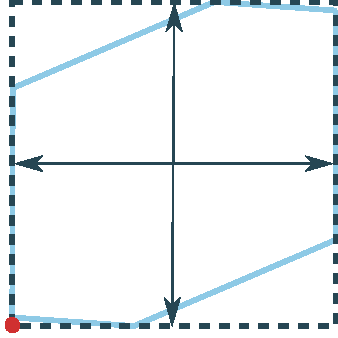
\includegraphics[width=0.8\linewidth]{graphics/surrogate_space_unit}
    \end{minipage}

\end{figure}
\end{mdframed}


\subsection{Visualizing transformations}
\label{sec:vis_trans}

The described transformation process can be visualized by illustrating where grid points from the lower dimensional space $\Omega_r$ would reside in the original input space $\Omega$. 
While it is normally not required to revert the previously shown transformation process, i.e. going from $\Omega_r$ back to $\Omega$, we require it for the visualization of transformed surrogates.

We observe that \cref{linear_trans} can be rearranged to solve for $p(x)$ to get
\begin{equation}
p(x)=2 G (t_{W_r}(x) - c_r)=2 Q ~ \text{diag}(s_1, \dots, s_r) ~ (t_{W_r}(x) - c_r).
\label{proj}
\end{equation}
To reverse the transformation completely, we have to deal with reversing $p(x)$ and the fact that in many cases, the inverse $p^{-1}(x_p)=\{x \in \Omega \mid p(x)=x_{p}\}$ function is not injective, because $|p^{-1}(x_p)| > 1$.
Our goal is to reverse the transformation only onto certain representative elements of the equivalence classes $[x]_p=\{x \in \Omega \mid p(x)=x_{p}\}$.
We then only consider the points
\begin{equation}
C \coloneqq \{x - c_d  \in \text{span} ~ W_r \mid x \in \Omega\},
\label{proj_rep}
\end{equation}
i.e. who lie in the vector subspace that is spanned by the active directions in $W_r$ and crosses the center $c_d$.
Next, we reverse the projection $p(x)$ only onto the representative elements $x \in C$, so that we are able to map one element $x_r\in \Omega_r$ onto one element $x \in C$ to obtain $t_{W_r}^{\text{reverse}}\colon \Omega_r \mapsto C$ with
\begin{equation}
t_{W_r}^{\text{reverse}}(x_r) \coloneqq ~W_r Q ~ \text{diag}\left(2s_1, \dots, 2s_r\right) (x_r - c_r) + c_d.
\end{equation}

This function is called a reverse function, as it is not a true inverse of $t_{W_r}$.
In \cref{fig:trans_vis} we reverse the grid points of a regular two-dimensional sparse grid lying in $\Omega_r$ onto a plane in the original three dimensional space $\Omega$ with the help of equation \cref{proj} and \cref{proj_rep}.

\begin{mdframed}[style=style]
\vspace{2.5mm}
\begin{figure}[H]
\begin{subfigure}{.5\textwidth}
  \centering
  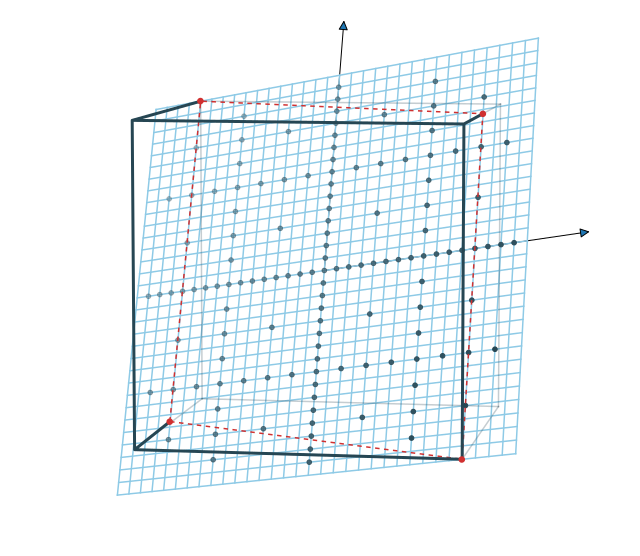
\includegraphics[width=\linewidth]{graphics/surrogate_vis_2}
\end{subfigure}%
\begin{subfigure}{.5\textwidth}
  \centering
  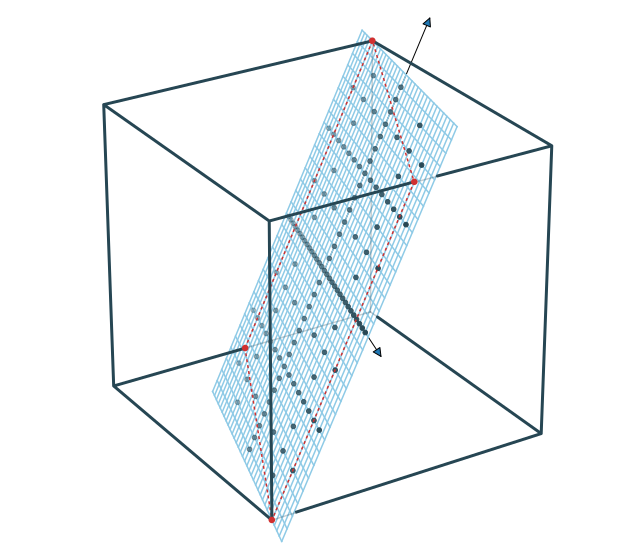
\includegraphics[width=\linewidth]{graphics/surrogate_vis_1}
\end{subfigure}
\vspace{2.5mm}
\delimit
\captionof{figure}{Two views of the same visualization of a transformed regular sparse grid of level $5$ that was constructed by a linear transformation with $r=2$ and $d=3$.\\
The \darkblue cube outline represents the edges of $\Omega$, the arrows on the sparse grid the first two column vectors of $W_r$ that span the plane on which the sparse grid and $\Omega_r$ lies, and the \red edges represent the intersections of $\Omega$ and the plane of $\Omega_r$.}
\label{fig:trans_vis}
\end{figure}
\end{mdframed}

\section{Active Subspaces}
\label{sec:as}

The method of active subspaces \cite{CG15} aims to identify the most influential directions in the parameter space to construct a lower-dimensional subspace of $\Omega$ that covers most of a models output variance to conduct parameter studies with a reduced amount of dimensions.
In constrast to conducting parameter studies, we will use the so-called active directions of a computed active subspace to construct the transformation matrix $W_r$.
Let
\begin{equation}
C \coloneqq \int_{\Omega} (\nabla f) (\nabla f)^T \rho ~ dx
\label{eq:as_c}
\end{equation}

be the average outer product of the gradient, a $(d \times d)$ matrix.
Since $C$ is a positive semi-definite matrix, it is possible to decompose it into its eigenvectors $v_i$ and their corresponding real eigenvalues $\lambda_i$ with
\begin{equation}
C = V \Lambda V^T, ~~ \Lambda \coloneqq diag(\lambda_1, \dots, \lambda_d), ~~ V \coloneqq
  \begin{bmatrix}
  \\
    v_1 ~ v_2 ~ \dots ~ v_{d-1} ~ v_d\\
    \\
  \end{bmatrix}.
\nonumber
\end{equation}

We furthermore assume that the eigenvectors in this decomposition are ordered, i.e. $\lambda_1 \geq \dots \geq \lambda_d$.
A larger eigenvalue indicates a higher rate of change along the direction, more precisely it is the average squared directional derivative of f with respect to its eigenvector $v_i$ \cite{CG14} with
\begin{equation}
\lambda_i=\mathds{E}[((\nabla f)^T v_i)^2]
\label{eigenvalues}
\end{equation}

Therefore, the column vectors of the matrix $V$ are ordered from most the active direction $v_1$ to least the active direction $v_d$.
By keeping only a specific amount of the most active directions $r \leq d$ we obtain the transformation matrix
\begin{equation}
W_r=\begin{bmatrix}
  \\
    v_1 ~ v_2 ~ \dots ~ v_{i-1} ~ v_r\\
    \\
  \end{bmatrix}
\label{basis}
\end{equation}

In the context of this thesis, the given input sample $\{x_1, \dots, x_n\}$ is used to derive the matrix $C$ from \cref{eq:as_c} using a classical Monte-Carlo approach from \cite{}.
The matrix $C$ can then be approximated with
\begin{equation}
C \approx \frac{1}{n} \sum_{i=1}^n  (\nabla f(x_i)) (\nabla f(x_i))^T
\label{eq:as_c_approx}
\end{equation}

\subsection{Estimating gradients for active subspaces}
\label{sec:as_est}

One superficial downside of the active subspace method is that gradients are required to approximate the matrix $C$ in \cref{eq:as_c_approx}.
In cases where the gradient function is not known and can not be easily computed, this would seem like a limiting factor is the feasability of active subspaces.
However, as this section will show, the gradients can be approximated in various ways from the available input data in ways that allows for a acceptable active subspace approximation.
The approximated gradients are then used as inputs for equation c\cref{eq:as_c_approx} to obtain the approximated active subspace matrix.
There are various different methods of achieving that, where each method has its advantages and disadvantages.

\subsection{Finite differences}

The most common approach to estimate the gradients are finite differences.
In this thesis, an adaptive mix of forward and backward differences with a fixed distance $h$ are used, where the range of possible spacing is constrained by $0 < h \leq 0.5$:

\begin{equation}
\frac{\partial f(x)}{\partial x_i} \approx
\begin{cases}
    \dfrac{f(x_1, \dots, x_i + h, \dots, x_d) - f(x)}{h}, & x_i + h \leq 1 \\[1.5em]
    \dfrac{f(x_1, \dots, x_i - h, \dots, x_d) - f(x)}{h}, & \text{else}
\end{cases}
\end{equation}

The downside in the context of the sample-based approach is the requirement to additionally evaluate the model function at $d$ other inputs to determine the gradient at one sample point.
For high $d$ and a large amount of samples $n$, $dn$ function evaluations for finite differences may become too costly.

\subsection{Directional derivatives}

In cases where finite differences are not suitable, the gradients can be determined using a different approach that only works on a given input sample and does not require further function evaluations.
The approach is to roughly approximate the gradient by looking at neighboring points in the same sample and using directional derivatives to create a system of linear equations for the gradient at a certain input.
Given two inputs $x, y \in \Omega, x \neq y$, we define the distance between the two inputs as $r=y-x$.
By extrapolating the gradient along the direction in a linear fashion, we can define an approximation rule with

\begin{equation}
r \nabla_x f \approx f(y) - f(x)
\end{equation}

Using $m \in \mathds{N}$ neighbours of a sample point $x \in \Omega$ with $y_i \in \Omega \setminus \{x\}, ~ i \in \{1, \dots, m\}$, we can create a system of linear equations with

\begin{equation}
\begin{bmatrix}
    y_1 - x\\
    \vdots \\
    y_m - x
  \end{bmatrix}  \nabla_x f =\begin{bmatrix}
    f(y_1) - f(x) \\ \vdots \\  f(y_m) - f(x)
    \\
  \end{bmatrix}
  \label{eq:dd_sle}
\end{equation}

One limitation of this calculation is the linear nature of the computed gradients, i.e. estimating gradients of a non-linear function can lead to biased gradients.
Furthermore, the choice of the $y_i$ heavily influences the result as well as the size of $m$.
The next sections introduce different ways of choosing the neighbours $y_i$ and also evaluate the results.


\paragraph{Random neighbour approximation}
The random neighbour approximation method takes as an input a subsample $S_{\text{rn}} \subseteq S \setminus \{x\}$ with $|S_{\text{rn}}|=m < n$.
The set $S_{\text{rn}}=\{y_1, \dots, y_{m}\}$ is called a random neighbour set of $x$.
This random neighbour set is then used as an input for equation \cref{eq:dd_sle} to approximate the gradient $\nabla_x f$.

For $n,m \to \infty$, the approximated gradient does not converge to the actual gradients, since the expected distance to the neighbours in a random neighbour set does not go to zero.
The problem of determining average neighbour distance is related to finding the mean line segment length $\Delta (d)$ in a d-dimensional unit hypercube \cite{Bailey2007}.
There is no closed form solution for $\Delta (d)$, but several approximations have been made for various dimensions \cite{Weisstein}, e.g. $\Delta (1)=\frac{1}{3}$, $\Delta (2)=0.52$, $\Delta (3)=0.66$.

\paragraph{Nearest neighbour approximation}
The nearest neighbour variant picks a subset $S' \subseteq S \setminus \{x\}$ with a manageable size $n'=|S'|$ similar the the random neighbour method and then calculates the $m \leq n'$ nearest neighbours $S_{\text{nn}}=\{y_1,\dots,y_m\} \subseteq S'$ of the point $x$ with $\|(y_1-x)\|_2 < \|(y_2-x)\|_2< \dots<\|(y_{m-1}-x)\|_2 < \|(y_{m}-x)\|_2$.

Compared to the random neighbour approximation, for $n,n',m \to \infty$, the approximated gradient does converge to the actual gradient, since the expected distance to the neighbours does go to zero.
However, this property comes at the cost of having to sort the available $n'$ neighbours by distance to pick the $m$ closest ones.
The parameters $n'$ and $m$ also have to be chosen carefully, as a unsuitable comination of $n'$ and $m$ would increase the average distance to the neighbours again so that the effect of chosing the nearest neighbours would diminish.

\newpage
\begin{mdframed}[style=style]
\vspace{2mm}
\begin{figure}[H]
  \centering
\begin{subfigure}{.45\textwidth}
  \centering
  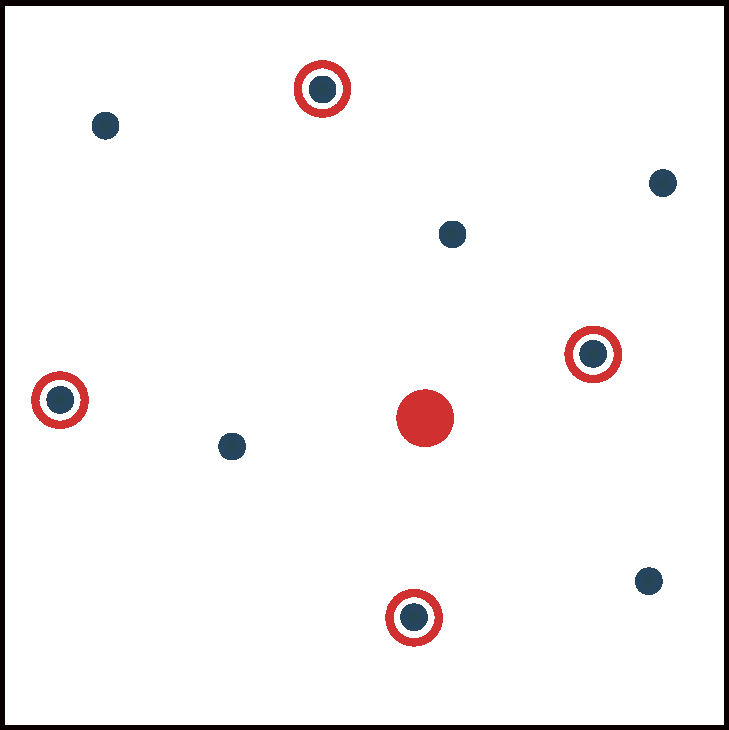
\includegraphics[width=.8\linewidth]{graphics/as_rn}
  \captionof{figure}{Random neighbour method picks with $m=4$}
  \label{fig:as_rn}
\end{subfigure}%
\begin{subfigure}{.45\textwidth}
  \centering
  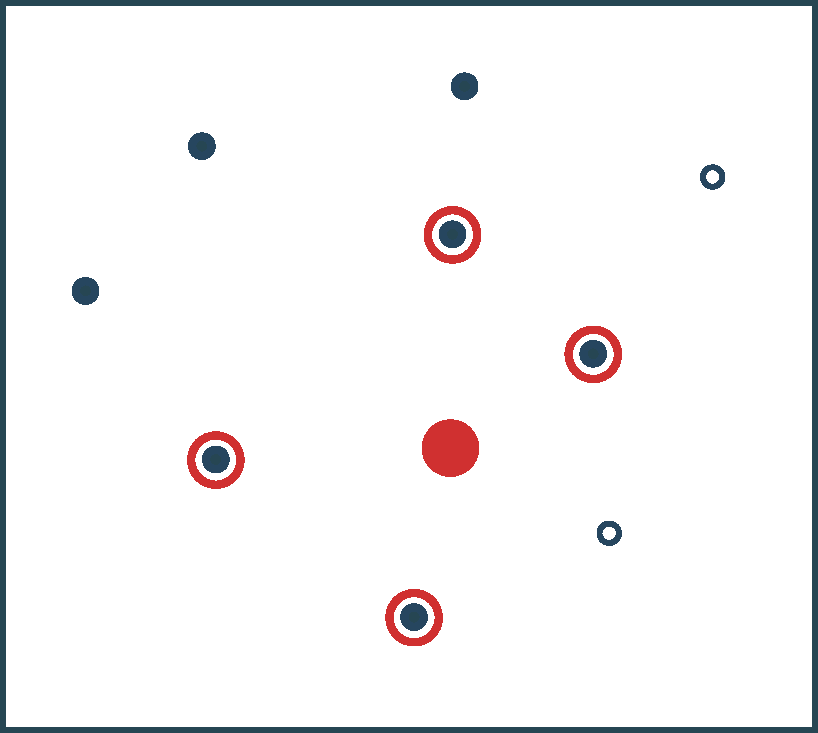
\includegraphics[width=.8\linewidth]{graphics/as_nn}
  \captionof{figure}{Nearest neighbour method picks with $n'=7$ and $m=4$}
  \label{fig:as_nn}
\end{subfigure}
\delimit
\captionof{figure}{Differences in sample selection between the two neighbour approximation methods for examples with $|S|=10$.
The \darkblue dots are the available samples $S \setminus \{x\}$. A filled dot signals that it is considered when looking for neighbours.
The completely \red circle represents the sample point $x$ and other sample points circled in \red indicate that they were chosen as a neighbour of $x$.}
\label{fig:as_approx}
\end{figure}
\end{mdframed}

\subsection{Limitations}
\label{sec:asl}

Active subspaces are however not a perfect indicator on which active directions are suitable for a linear transformation construction, since they can be misled.
A larger eigenvalue indicates a higher rate of change along the direction, more precisely it represents the average squared directional derivative of $f$ with respect to its eigenvector $v_i$ with $\lambda_i=\mathds{E}[((\nabla f)^T v_i)^2]$ \cite{CG14}.
However, a high rate of average squared change does not necessarily indicate that a direction $v_i$ is worth keeping.
For example, we can create the simple function
\begin{equation}
f(x_1, x_2)=10x_1 + \frac{1}{10} \sin(100 \pi x_2)
\end{equation}
that illustrates the limitations of active subspaces.
The optimal active direction worth keeping would be the first component only, as the second term can be seen as a highly changing noise term that does not effect the approximation error a lot if removed, as the amplitude of the sinus is small.
However, as the average squared directional derivative along the second dimension $(0,1)^T$ is way higher than along the first $(1,0)^T$, the calculated active subspace is biased heavily along the second dimension.

A positive aspect of the active subspace approximation methods is that they introduce a regularization through discretization \cite{Kress1999}, i.e. as the distances between neighbours are comparatively high, they discard noise terms with high frequencies such as the one shown in the previous example.
In certain cases, like the example function presented in this section, this will lead to better function approximations for neighbour approximation methods compared to alternatives such as given gradients and finite differences.

\section{Random linear transformations}
\label{sec:rt}

A completely different approach to finding a transformation function is just generating a random one.
A random transformation generator is easy to implement, can generate new transformation functions almost instantly and offers a purely exploratory approach to finding the best transformation.
It can also serve as a reference for comparision as one would expect that the Active Subspace method should always output better transformation.

A simple generation algorithm would first generate random matrices $R \in \mathds{R}^{d \times d}$ until all column vectors are significantly linear independent, and then orthonormalizing $R$ using the Gram-Schmidt method on the column vectors $r_i$ of $R$ to obtain the column vectors
\begin{equation}
w_i=\frac{w_i'}{\| w_i' \|},~~ w_i'=r_i - \sum_{k=1}^{i-1} \frac{\langle r_k,  w_k' \rangle}{\langle w_k', w_k' \rangle} w_k'
\end{equation}
and therefore the orthonormal matrix
\begin{equation}
W = \begin{bmatrix}
  \\
    w_1 ~ w_2 ~ \dots ~ w_{r-1} ~ w_d\\
    \\
  \end{bmatrix}.
\end{equation}
The final step would randomly roll a value for $1 \leq r \leq d$ and cut off the last $d-r$ column vectors of $W$ to obtain the transformation matrix
\begin{equation}
W_r = \begin{bmatrix}
  \\
    w_1 ~ w_2 ~ \dots ~ w_{r-1} ~ w_r\\
    \\
  \end{bmatrix}.
\end{equation}
Note that although the generated random orthonormal matrices are perfectly uniformly distributed in the orthogonal group $O(d)$ and we would need a different algorithm to achieve a true uniform distribution \cite{Wang2008}, they are still perfectly usable for the purpose of input transformations.

\section{Alternative transformations}

Until now, the focus lied primarily on deterministic linear transformations, because they are relatively easy to use and construct with the help of active subspaces.
However, in theory we can construct and use arbitrary transformation functions.
This section will briefly cover a few alternative types of transformations that are not the primary focus of this thesis, but do show some potential that could be investigated further.

\subsection{Periodic transformations}

Another possible use case for transformations are periodic functions.
If the model function $f$ is for example approximately periodic along one dimension $i$ with the period $p_i$, i.e. it holds that $f(x_1,\dots,x_i,\dots,x_d) \approx f(x_1,\dots,x_i + p_i, \dots,x_d)$, we can easiliy define a transformation function
\begin{equation}
t_{\text{periodic}}(x_1,\dots,x_i,\dots,x_d) \coloneqq (x_1,\dots, \frac{x_i\text{ mod } p_i}{p_i}, \dots,x_d)^T
\label{eq:per}
\end{equation}
and create a normal surrogate $\hat{f}$ on $\Omega$ with $f(x) \approx \hat{f}(t(x))$.
This way, the function can be interpolated better by sparse grids because there are effectively $1 / p_i$ times more grid points spent along the $i$-th dimension.
However, no dimension reduction is taking place.
Of course this can concept can be expanded upon with handling multiple periodic dimensions at once, antiperiodic functions, offsets and combination with linear transformations.

A simple example would be the periodic function $f_p(x)=\sin(16\pi x_1)  + \cos(16\pi x_2)$, which repeats in intervals of $\frac{1}{8}$ along both dimensions.
This can be exploited by constructing a periodic transformation with $p=p_1=p_2=\frac{1}{8}$ as shown in \cref{eq:per} by using the transformation
\begin{equation}
t_p(x_1,x_2) \coloneqq \left[\frac{1}{p} \left(x_1 \text{ mod } p\right), \frac{1}{p} \left(x_2 \text{ mod } p\right)\right]^T.
\nonumber
\end{equation}

\begin{mdframed}[style=style]
\vspace{2mm}
\begin{figure}[H]
        \centering
\begin{minipage}{.4\textwidth}
        \centering
  \captionof{figure}{Approximation errors of various periodic transformations $t_p$ and sparse grid surrogates of level $\ell \in \{1, \dots, 11\}$, modified linear hat basis, and periods $p \in \{\frac{1}{8}, \frac{1}{4}, \frac{1}{2}, 1\}$ for the example function $f$.\\
  The sparse grid surrogates were constructed using the normal interpolation approach.}
    \end{minipage}%
    \begin{minipage}{0.6\textwidth}
        \centering
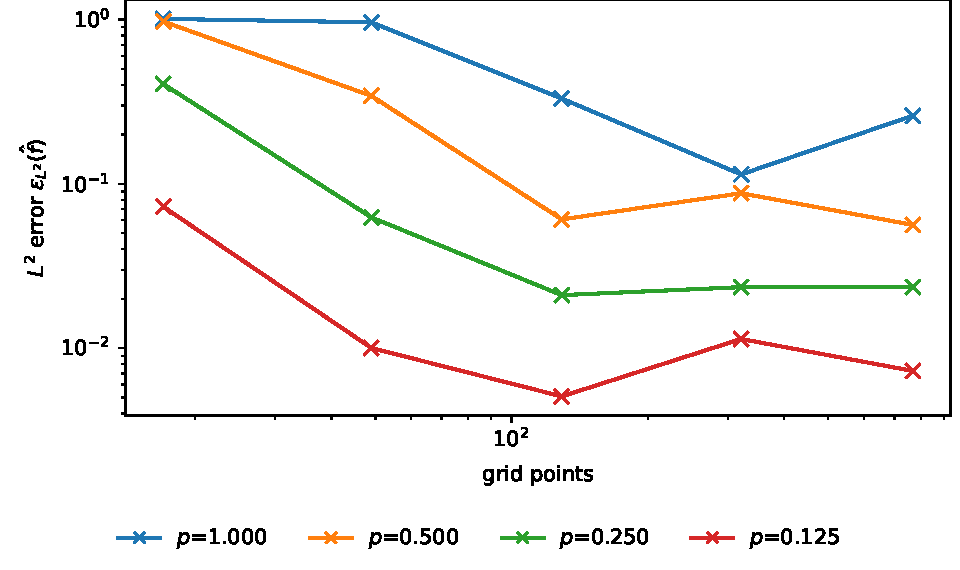
\includegraphics[width=0.85\textwidth]{graphics/periodic}
    \end{minipage}
\label{fig:periodic}
\end{figure}
\end{mdframed}

To illustrate the improvement in multiple smaller steps, we investigate periodic transformations with several configurations in \cref{fig:periodic}.
As we can see, a smaller value for $p$ results in a notable improvement, and going from $p=1$ (no transformation) to $p=0.125$ (best periodic transformation) improves the approximation error by around $10^2$, which is a huge improvement after all.

\subsection{Manifolds}

Another approach to create more flexible transformations that can, at least in theory, also exploit nonlinear structures are manifold-based methods:

\paragraph{Active Manifolds}
Inspired from active subspaces, which are purely linear in their nature, one can extend the concept to identifying a one-dimensional curve in the domain $\Omega$ along the flow of most active change, which is called an active manifold \cite{Bridges2019}.
Compared to Active Subspaces, calculating the Active Manifold is more complex and resource intensive.
Furthermore, defining a transformation function that maps from $\Omega$ onto the local one-dimensional space of the curve is way more complex and can be constructed in many ways.
Also they are currently limited to one dimension, for which the surrogate construction method becomes pretty irrelevant.

\paragraph{Principal Manifolds}
A similar concept to active manifolds are principal manifolds \cite{Huo}.
They are an extension to the principal component analysis \cite{Abdi2010}, which can only compute linear principal components.
These are able to construct nonlinear multi-dimensional manifolds and are therefore more powerful than active manifolds.
The inputs that are then projected onto the principal manifold such that a surrogate can be created for the projected inputs, similar to the presented linear transformation approach in this thesis.
Such an approach has already been investigated in \cite{Feuersaenger2009}.

\paragraph{}
The foreseeable main limitation of the application of nonlinear manifolds in conjunction with sparse grids is that the axis-aligned nature can no longer be adjusted to the model function.
The transformation of inputs based on an orthonormal matrix preserves angles and allows to orientate the inputs more optimal 

\chapter{Transformed surrogates}
\label{chap:c4}

Once a transformation function $t(x)$ has been created, the next step is creating a surrogate in the reduced input space $\Omega_r$.
As we will see in this chapter, this is not trivial to do with sparse grids and requires special care as there are several challenges that come with the usage of input transformations.
Some of these are specific to sparse grids, while others are independent of the used surrogate type.

\section{Transformed input space}
\label{sec:tis}

All transformed inputs form the transformed input space, which is a part of the reduced surrogate space $\Omega_r$.
The transformation function was constructed in the last chapter in such a way that every transformed inputs lies in $\Omega_r$, while also applying scaling to use as much space of $\Omega_r$ as possible.
\begin{definition}[Transformed input space]
Let $t \colon \Omega \mapsto \Omega_r$ be transformation function.
We define the transformed input space as
\begin{equation}
T \coloneqq \{t(x) \mid x \in\Omega\}, ~~ T \subseteq \Omega_r.
\end{equation}
\end{definition}
The main difference between $T$ and $\Omega_r$ is that $\Omega_r$ is a unit hypercube, while $T$ might not be one.
As we will show later, in many cases $T$ is not a unit hypercube and it holds that $T \subset \Omega_r$.
We should strive to have $T$ cover $\Omega_r$ as much as possible to not make a portion of $\Omega_r$ go unused when constructing the surrogate.
\begin{definition}[Unusued reduced surrogate inputs]
Let $t \colon \Omega \mapsto \Omega_r$ be transformation function, and let $U_t=T \setminus \Omega_r$ be the unused reduced surrogate space.
Then
\begin{equation}
\tilde{u}_t \coloneqq \frac{|U_t|}{|\Omega_r|}
\end{equation}
is the share of unused inputs of the reduced surrogate space.
\end{definition}

The greater $U_t$ and therefore the unused input share $\tilde{u}_t$, the more grid points can potentially be generated outside of $T$, if sparse grids are created in a regular way instead of employing adaptivity.
Note that even if a grid point lies outside of $T$, it can still contribute to some degree to the approximation error of the surrogate if the support of the basis function $\phi$ intersects with $T$.
Thus, grid points are only completely unused if their basis function support does not intersect with $T$.
Other surrogate types do not have the same issue, as radial basis functions for example can freely choose their support points and therefore automatically adapt to $T$.

\section{Method selection}
\label{sec:ms}

Usually, the standard sparse grid technique makes use of the sparse grid interpolation method, which is able to generate an accurate interpolant quickly as described in \cref{sec:gsc}.
However, as we will show in this section, sparse grid interpolation is not suitable for many scenarios with transformed sparse grids and we will therefore differentiate between two cases.
If it holds that $r=d$, i.e. we do not perform a dimension reduction, the transformation can be seen as orientation changing only.
In that case, if a linear transformation is created according to the rules of the previous chapter s.t. all inputs are transformed into a unit hypercube with equal dimension, the transformation function is injective and it maps from $\Omega$ into $T \subseteq \Omega$.
\Cref{fig:aligned_grid} illustrates this case.

\begin{mdframed}[style=style]
\begin{figure}[H]
        \centering
\begin{minipage}{.49\textwidth}
        \centering
  \captionof{figure}{Illustration of a possible case with $r=d=2$. The \beige square represents $\Omega=\Omega_r$, the black dots are the grid points of a sparse grid surrogate, and the rotated \lightblue square is $T$. The \grey square in top right corner represents the support of the grid point in its center.}
\label{fig:aligned_grid}
    \end{minipage}%
    \begin{minipage}{0.49\textwidth}
        \centering
   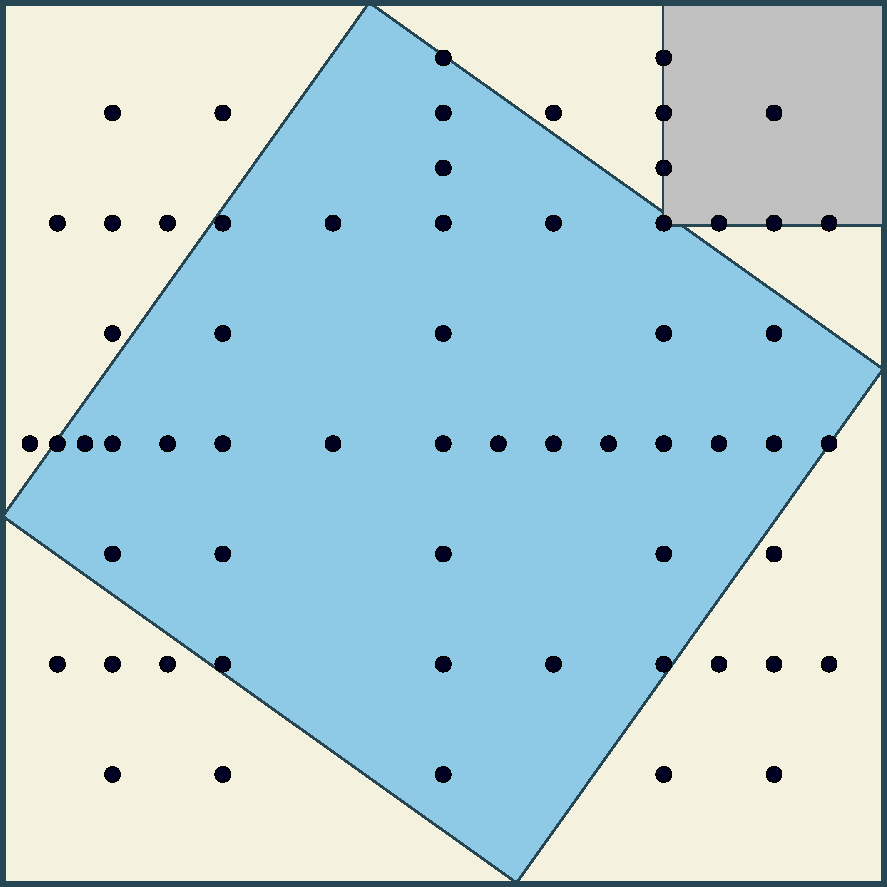
\includegraphics[width=0.8\linewidth]{graphics/aligned_grid}
    \end{minipage}
\end{figure}
\end{mdframed}

It is possible to use normal sparse grid interpolation to create a surrogate for the transformation, if we define how to treat function evaluations for grid points outside of $\Omega$.
For that we can either define a rule on how to treat these function evaluations, or ensure that grid points outside of $T$ never are created.
Restricting grid point creation in $U_t$ is difficult as the grid point hierarchy, which dictates that every grid point has a parent, should be kept intact to work effectively with a sparse grid.
Thus, restricting grid point creation in $U_t$ can prevent large areas in $\Omega$ not being covered by grid points as a basic parent grid point might lie outside of $T$.
Note that even if there are many grid points that were generated outside of $T$, as seen in figure \cref{fig:aligned_grid}, no grid point is actually completely unused, as the support of every grid point basis function intersects at least barely with $T$ and contributes to the approximation error.

The alternative approach would first require to create a modified model function $f' \colon \mathds{R}^d \mapsto \mathds{R}$ that can be evaluated outside of $\Omega$.
We can either set all values outside $\Omega$ to 0 with
\begin{equation}
f'_0(x) \coloneqq \begin{cases}
f(x)&, \text{if $x \in \Omega$}\\
0&,\text{else}
\end{cases}
\end{equation}
or just extend the input domain to allow the model function to be evaluated outside of $\Omega$ with $f'_{\text{ext}}(x) \coloneqq f(x)$.
As the transformation function is an automorphism of $\Omega$ when $r=d$, it is invertible for elements $t \in T$ and the inverse function $t^{-1} \colon T \mapsto \Omega$ can easily be constructed as $t$ is linear.
We can extend the inverse transformation $t^{-1}$ to accept all elements $x \in \Omega$ without a problem with $t^{-1}_{\text{ext}} \colon \Omega \mapsto \mathds{R}^d$ and use it to create the function $\tilde{f}(x)=f'(t^{-1}_{\text{ext}}(x))$ that can be used for sparse grid interpolant creation.

However, if we perform a dimension reduction with $r < d$, we can no longer effectively make use of sparse grid interpolation as the transformation is longer invertible because many inputs can be projected onto one point with $t(x_i)=\dots=t(x_j)$.
We are then dealing with data that might be, depending on the model function and the transformation, very noisy and there also might be multiple different values for the same inputs, with
\begin{equation}
t(x_i)=t(x_j), ~ f(x_i) \neq f(x_j), ~ x_i \neq x_j
\end{equation}
As a result, the transformed surrogate construction is usually an ill-posed problem for $r < d$, and we have to employ sparse grid based regression methods to successfully create a surrogate for the transformed data.

\begin{mdframed}[style=style]
\begin{figure}[H]
        \centering
\begin{minipage}{.45\textwidth}
        \centering
  \captionof{figure}{Illustration of a possible case with $r=1$ and $d=2$.
  The surrounding \beige square represents $\Omega$, the \lightblue line represents $\Omega_r=T$, the black dots are the grid points of the sparse grid surrogate.
The \green points are sample points that are being mapped from $\Omega$ onto $\Omega_r$.
Note that as $\Omega$ and $\Omega_r$ are distinct vector spaces, this figure visualizes the one dimensional $\Omega_r$ as the elements crossing the center in the same way as \cref{sec:vis_trans}.}
    \end{minipage}%
    \begin{minipage}{0.55\textwidth}
        \centering
   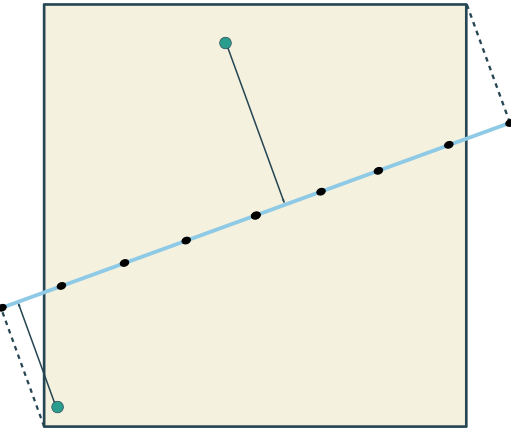
\includegraphics[width=0.85\linewidth]{graphics/reduced_grid}
\label{fig:reduced_grid}
    \end{minipage}
\end{figure}
\end{mdframed}

The interpolation based approach will however not be used or investigated in this thesis, as the focus lies on cases with $r < d$ and the regression approach also being able to handle the case with $r=d$.
It is however a certainly interesting approach worthy of being investigated further mainly with the goal of improving the approximation errors for sparse grid interpolants even further.

\section{Sparse grid regression}

The original function samples
\begin{equation}
S \coloneqq \{(x_1, f(x_1), \dots, (x_n, f(x_n))\} \subseteq \Omega \times \mathds{R}
\end{equation}
that were drawn randomly from to the given input probability distribution $\rho$, are transformed to obtain the transformed sample
\begin{equation}
S_t \coloneqq \{(t(x_1), f(x_1), \dots, (t(x_n), f(x_n))\} \subseteq T \times \mathds{R}.
\end{equation}
We are aiming to construct the surrogate function $\hat{f}_t$ using sparse grids with the sparse grid point set $X$ and basis functions $\phi_{\underline{l},\underline{i}}$ for the transformed sample $S_t$ with
\begin{equation}
\hat{f}_t(x) \coloneqq \sum_{x_{\underline{l},\underline{i}} \in X} \alpha_{\underline{l},\underline{i}} \phi_{\underline{l},\underline{i}}(x)
\end{equation}

The basic approach would be to solve the least squares problem with the standard square loss function
\begin{equation}
\varepsilon_{\text{MSE}}(\hat{f}_t)=\frac{1}{n} \sum_{i=1}^n (f(x_i) - \hat{f}_r(t(x_i)))^2 
\end{equation}

Since the surrogate construction for a transformation is usually an ill-posed problem, might contain random noise, and we are calculating a regressed function only based on the transformed samples $S_t$, the regression method used employs regularization as well to prevent overfitting.
We are therefore solving the regularized least squares problem with the smoothing factor $\lambda > 0$:
\begin{equation}
\hat{f}_t^{\lambda^*} = \argmin_{\hat{f}_r^\lambda \in V} \epsilon(\hat{f}_r^\lambda) + \lambda R(\hat{f}_r^\lambda)
\end{equation}

Compared to sparse grid interpolation, the regression method takes longer to construct a well fitting surrogate as an optimization problem that involves all grid points has to be solved.
The regression algorithm also provides the ability to make use of spatially adaptivity to refine the grid in areas where the difference between surrogate value and training data $\hat{f}_t(x_i) - f(x_i)$ is large.


\section{Multifidelity surrogates}
\label{sec:lofi}

The construction of the best possible Sparse Grid surrogate, given a function sample, a transformation, and set of possible configuration parameters can become very computationally expensive, since every parameter combination has to be evaluated to determine the best one.
To mitigate this problem, we employ the concept of multifidelity simulations \cite{Robinson2006}, i.e. reducing the cost of parametrization by using low fidelity Sparse Grids and datasets to evaluate a parameter combination and only using high fidelity Sparse Grids and datasets when creating the final surrogate using the determined to be optimal parameters.

A low fidelity Sparse Grid surrogate $\hat{f}^l$ has less grid points compared to an otherwise identical high fidelity Sparse Grid surrogate $\hat{f}^h$.
This means that the level of $\hat{f}^l$ is lower and less or not refinements at all are used.
It is vital that the used low fidelity surrogates still stay comparable when evaluating the errors for different parameter combinations.
They don't have to be representative of the high fidelity surrogate error, but should fullfil the following property:
\begin{equation}
\varepsilon(\hat{f}_1^l) < \varepsilon(\hat{f}_2^l) \Rightarrow \varepsilon(\hat{f}_1^h) < \varepsilon(\hat{f}_2^h)
\end{equation}
i.e. they should be indicative of the comparative quality of their high fidelity surrogates for an error metric.

This multifidelity approach will also be used in later chapters in a more extensive fashion to also evaluate multiple different transformations to choose the best one.
The ability to evaluate quickly transformations is especially critical for the random transformation method, as it allows for the generation and evaluation of many transformations to choose the best from.

\section{Operations on transformed surrogates}

Now that a surrogate has been created and we can approximate the model function with $f(x) \approx \hat{f}_t(t(x))$,
we can look at the differences when working with transformed surrogates compared to the standard case of sparse grid interpolation surrogates without using a transformation function in between.

\paragraph{Differentiation}
Assuming that the surrogate uses a basis that can be differentiated easily, such as B-Splines, the gradient can be approximated using the chain rule and the gradient function of the transformed surrogate with
\begin{equation}
\nabla f(x) \approx \nabla \hat{f}_t(t(x)) = \nabla (\hat{f}_t \circ t)(x)=(Dt(x))^T \nabla \hat{f}_t(t(x)).
\end{equation}
For a linear transformation, $Dt(x)$ can easily be calculated and we can therefore perform a differentation just as before.

\paragraph{Optimization}
To calculate the maximum $x^\text{max} \coloneqq \argmax_{x \in \Omega} f(x)$ or minimum $x^\text{min} \coloneqq \argmin_{x \in \Omega} f(x)$ of the model function, one can also optimize the surrogate. There exist many different algorithms, especially for B-Spline basis functions presented in \cite{}.
However, we have to keep in mind that not every element $x_r \in \Omega_r$ is actually transformed onto, i.e. some $x_r \notin T$.
Therefore a constrained optimization has to be performed on the surrogate first with
\begin{equation}
x_{r}^\text{max} \coloneqq \argmax_{x_r \in \Omega_r} \hat{f}(x_r), ~ x_r \in T.
\end{equation}

Afterwards, at least in the dimensionality preserving transformation with $r=d$, we then can obtain the maximum $x^\text{max}$ with $x^\text{max}=t^{-1}(x_{r}^\text{max})$, since $x_{r}^\text{max} \in T$.
One problem is that in the case of a reducing transformation with $r<d$, a computed surrogate maximum $x_{r}^\text{max}$ may be a set of many points.
Therefore another non sparse grid based optimization can be performed on the set $t^{-1}(x_{r}^\text{max})$, to get a good maximum estimate.

\paragraph{Quadrature}
Given an input distribution $\rho$ and transformation $t$, we can compute the integral with
\begin{equation}
\int_{\Omega} f(x) \rho(x) \; \text{d}x \approx \int_{\Omega} \hat{f}_t(t(x)) \rho(x) \; \text{d}x
=
\int_{\Omega_r} \hat{f}_t(z) \left(\int_{t^{\text{inv}}(z)} \rho(x)  \; \text{d}x \right)  \; \text{d}z=
\int_{\Omega_r} \hat{f}_t(z) \rho_t(z) \; \text{d}z
\end{equation}
By introducing a transformation we lose the ability to easily use Sparse Grid based quadrature algorithms, as the distribution $\rho_t$ is not a simple distribution.
However, since $r$ is usually a lot smaller than $d$, Monte-Carlo based quadrature becomes a better option for transformed surrogates as the curse of dimensionality is weakened that way.
This also holds true for cases with a uniform input distribution $\rho=\mathcal{U}(0,1)^d$ as the $\rho_t$ is usually no longer a uniform distribution.


\chapter{Iterative transformations}
\label{chap:c5}

We now covered all the required steps to approximate a model function with a transformed surrogate, which in this thesis mainly happens to be a transformed sparse grid.
However, we can easily see that using just one transformed surrogate for approximation is not as powerful as it needs to be for many models.
In many cases, an iterative approach that generates a sum of multiple different transformed surrogates suits a model function better than a single one, especially if the model function is a sum of function terms itself.
We can adapt \cref{def:intrinsic} for the intrinsic dimension, to obtain a dimension for effective intrinsic dimension:

\begin{definition}[Compounded intrinsic dimension]
A $d$-dimensional function $f(x_1, \dots, x_d)$ has a compounded intrinsic dimension of $r \leq d$, if there exist transformation functions $t_i \colon \Omega \mapsto \Omega_{r_i}$ and functions $f_i \colon \Omega_{r_i} \mapsto \mathds{R}$, such that
\begin{equation}
\forall x \in \Omega \colon f(x)=\sum_{i=1}^p f_{t_i}(t_i(x))
\end{equation}
and $r=\max r_i$.
\label{def:intrinsic_sum}
\end{definition}
%
For example, having multiple surrogates allows us to approximate model functions that consist out of multiple terms with a low effective intrinsic dimension, such as $f(x_1, x_2)=\sin(2 \pi x_1) + x_2$, which consists out of two terms with an intrinsic dimension of $1$ and therefore also a compounded intrinsic dimension of $1$.
The notion of compounded intrinsic dimension is more powerful than normal intrinsic dimension, as it also covers any sum of function terms, and we will need for iterative transformations.

\section{Projection pursuit regression}

If we take a look at similar dimension reduction methods and take some inspirations from them, we can see that one of these insightful related methods is projection pursuit regression \cite{huber1985projection}.
The projection pursuit regression method comes from the area of statistics and is in its core idea related to our approach with linear transformations.
It tries to represent a dataset
\begin{equation}
P \coloneqq \{(x_i, y_i)\}=\{(x_i, f(x_i))\}
\end{equation}
using the form
\begin{equation}
y_i=\beta_0 + \sum_{k=1}^m f_k(\beta_k^T x_i) + \varepsilon_i
\label{eq:ppr}
\end{equation}
where $\beta_0$ is a constant, $\beta_k$ are projection matrices, the $f_k$ are lower dimensional function surrogates, and the $\epsilon_i$ are the residiuals.
Using the $\beta_k$ to project inputs onto a lower-dimensional space is very similar to our concept of creating linear transformations.
The functions $f_k$ and projection matrices $\beta_k$ of this additive model can then be calculated iteratively by applying one step of finding a projection and constructing a surrogate repeatedly each time on the error function
\begin{equation}
e_k(x) \coloneqq f(x) - \sum_{i=1}^k f_k(\beta_k^T x)
\end{equation}
%
This term can be computed using an iterative approach, as seen in \cref{alg:ppr}.

\begin{mdframed}[style=algstyle,frametitle={\textbf{function} \texttt{projectionPursuitRegression}{$(f, k_{\text{max}})$}}]
\normalsize
\vspace{5.5mm}
\begin{algorithmic}[1]

    \State $e_0 = f$
    \For{$k = 1, \dots, k_{\text{max}}$}
    	\State $\beta_k \gets$ \texttt{determineBestProjection}($e_k$)
    	\State $f_k \gets$ \texttt{determineBestSurrogate}($e_k, \beta_k$)
    	\State $e_k \gets e_{k - 1} - f_k$
    \EndFor
    \State $\hat{f}(x) \gets \sum_{f_k}^m f_k(\beta_k^T x)$
    \State \Return{$\hat{f}$}
\end{algorithmic}

\vspace{-1.5mm}
\delimit

	\captionof{algorithm}{Pseudocode of the iterative projection pursuit regression algorithm. Parameters are the function $f$ and the maximum amount of iterations $k_{\text{max}}$.}
	\label{alg:ppr}
\end{mdframed}
%
Alternatively, we could also introduce an error exit condition to \cref{alg:ppr} that exits the loop if the regression error is small enough with $\varepsilon(e_i) < \varepsilon_{max}$.
We can already spot that the function \texttt{determineBestProjection} relates to \cref{chap:c3}, where we extensively covered finding a linear transformation, and \texttt{determineBestSurrogate} relates to \cref{chap:c4}, which covered the creation of sparse grid surrogates for a given transformation.

\section{An iterative approach}

Going from this statistical model to our function approximation problem, we can formulate the same concept using the notation used in this thesis by dropping the constant term $\beta_0$ and residuals $\varepsilon_i$ from \cref{eq:ppr} to get

\begin{equation}
\hat{f}(x)=\sum_{i=1}^m \hat{f_{t_i}}(t_i(x_i)),
\nonumber
\end{equation}
%
where the $t_i$ are linear transformations similar to the projection with $\beta_k^T$, and the $\hat{f_{t_i}}$ are the surrogate equivalents of the $f_k$.
The functions $\hat{f_{t_i}}$ and transformations $t_i$ can then be constructed iteratively by repeatedly executing a stepwise algorithm of first finding a transformation and then constructing a surrogate for the current error function

\begin{equation}
e_k(x)=f(x) - \sum_{i=1}^k \hat{f_{t_i}}(t_i(x)).
\nonumber
\end{equation}
%
\Cref{alg:itappr} illustrates this iterative approach, which is similar to \cref{alg:ppr}, but has been adapted to fit our used notation.
In the case that we use a linear transformation function, \cref{alg:itappr} is pretty much identical to \cref{alg:ppr}.

\begin{mdframed}[style=algstyle,frametitle={\textbf{function} \texttt{transformedSurrogateSum}{$(f, i_{\text{max}})$}}]
\normalsize
\vspace{5.5mm}
\begin{algorithmic}[1]
    \State $e_0 = f$
    \For{$i = 1, \dots,  i_{\text{max}}$}
    	\State $t_i \gets$ \texttt{generateBestTransformation}($e_{i - 1}$)
    	\State $\hat{f}_{t_i} \gets$ \texttt{generateBestSurroate}($e_{i - 1}, t_i$)
    	\State $e_i \gets e_{i - 1} - \hat{f}_{t_i}$
    \EndFor
    \State $\hat{f} \gets \sum_{\hat{f}_{t_i}} \hat{f}_{t_i} \circ t_i$
    \State \Return{$\hat{f}$}
\end{algorithmic}
\vspace{-1.5mm}
\delimit
	\captionof{algorithm}{Pseudocode of the iterative transformed surrogate sum algorithm. Parameters are the model function $f$ and the maximum amount of iterations $i_{\text{max}}$.}
	\label{alg:itappr}
\end{mdframed}

\section{Generating the best surrogate}
\label{sec:gs}

Surrogates can, depending on their type, have possibly many independent configuration parameters, which can heavily influence the end result and therefore the approximation error.
The amount of possible configuration parameter combinations makes finding the best combination difficult, as it would require the examination of a lot of combinations and in most cases the actual surrogate has to be constructed with a given set of parameters to evaluate the suitability of the parameters.
The main driver of the runtime of the function \texttt{generateBestSurroate} is therefore the amount of configurations parameters available.
Common configuration parameters usually include regression parameters like the smoothing factor $\lambda$.
More formally assuming that we have $m$ configuration parameters where each one has a set of possible values $C_i$, the configuration set would be $C=C_1 \times \dots \times C_m$ and the amount of examinations would be $|C|=|C_1| \dots |C_m|$.

The general structure and properties of the current regression problem at hand can change with each new iteration.
Thus, configuration parameters have to examined in every iteration again, as their might not exist a set of optimal configuration parameters for all iterations.
\Cref{alg:bestsur} shows a simple implementation that uses lofi surrogates for parameter evaluation to reduce runtime.

\newpage
\begin{mdframed}[style=algstyle,frametitle={\textbf{function} \texttt{generateBestSurroate}{$(e, t)$}}]
\normalsize
\vspace{5.5mm}
\begin{algorithmic}[1]
    \State $c^\ast \gets \emptyset$
    \State $\varepsilon_{min} \gets \infty$
    \For{$c \in C$}
      \State $\hat{f}_c^l$ $\gets$ \texttt{generateLofiSurroate}($e, t, c$)
    	\State $\varepsilon \gets \varepsilon(\hat{f}_c^l)$
    	\If{$\varepsilon < \varepsilon_{min}$}
    	  \State $\varepsilon_{min}\gets \varepsilon$
    	\State $c^\ast \gets c$
    	\EndIf
    \EndFor
    \State \Return{\texttt{generateHifiSurroate}($e, t, c^\ast$)}
\end{algorithmic}
\vspace{-1.5mm}
\delimit
	\captionof{algorithm}{Pseudocode of the surrogate generation algorithm. The parameters are the current error function $e$ and the transformation function $t$. The the set of possible surrogate configurations $C$ is fixed.}
	\label{alg:bestsur}
\end{mdframed}
%
This algorithm determines the optimal configuration $c^\ast$ with
\begin{equation}
c^\ast \coloneqq \argmin_{c \in C} \varepsilon(\hat{f}_c^l)
\nonumber
\end{equation}
and works fine presuming that the low fidelity surrogates $\hat{f}_c^l$ are representative of the high fidelity ones, as already discussed in \cref{sec:lofi}.
It is satisfactory as long as the actual approximation quality of the generated hifi surrogate is close to the optimal configuration over all parameter combinations, i.e. it should hold that

\begin{equation}
\varepsilon(\hat{f}_{c^\ast}^h) \approx \argmin_{c \in C} \varepsilon(\hat{f}_c^h).
\nonumber
\end{equation}

\section{Generating the best transformation}

Until now, we assumed that the reduced dimension $r$ was given and did not cover ways on how to determine the optimal reduced dimension $r^\ast$, or the optimal $r^\ast_i$ for an iteration step.
It was mentioned that, when covering active subspaces in \cref{sec:as}, even though the active subspace method provides a suggested criterion to determine the optimal cutoff dimension $r^\ast$ by looking for the largest gap in the sequence of eigenvalues, this criterion was not always optimal and could be influenced by various factors.
Furthermore, alternative transformation generation methods, like random transformations in \cref{sec:rtg}, can not make use of such a cutoff criterion.
We are therefore looking a for a generalized approach to determine the best value for $r^\ast_i$ in each iteration.
One solution would be to use the exploratory look ahead approach to find the best configuration parameters from the previous section to determine the best $r^\ast_i$ in a similar fashion.

\newpage

\begin{mdframed}[style=algstyle,frametitle={\textbf{function} \texttt{generateBestTransformation}{$(e, r_{\text{min}} ,r_{\text{max}})$}}]
\normalsize
\vspace{5.5mm}
\begin{algorithmic}[1]
    \State $t^\ast \gets \mathds{1}$
    \State $\varepsilon_{min} \gets \infty$
    \For{$r = r_{\text{min}},\dots,r_{\text{max}}$}
      \State $t_r$ $\gets$ \texttt{generateTransformation}(e, r)
      \State $\hat{f}_{c^\ast}^h$ $\gets$ \texttt{generateBestSurroate}($e, t_r$)
    	\State $\varepsilon \gets \varepsilon(\hat{f}_c^h)$
    	\If{$\varepsilon < \varepsilon_{min}$}
    	  \State $\varepsilon_{min}\gets \varepsilon$
    	\State $t^\ast \gets t_r$
    	\EndIf
    \EndFor
    \State \Return{$t^\ast$}
\end{algorithmic}
\vspace{-1.5mm}
\delimit
	\captionof{algorithm}{Pseudocode of the transformation generation algorithm. Parameters are the current error function $e$, the minimum reduced dimension $r_{\text{min}}$, and maximum reduced dimension $r_{\text{max}}$.}
	\label{alg:besttrans}
\end{mdframed}
%
The function implementation of \texttt{generateTransformation} in \cref{alg:besttrans} is usually fixed, and can use one of the transformation generation methods presented in \cref{chap:c3}, for example active subspaces or random transformations.

\section{Visualizing the algorithm}

The iterative algorithm can be visualized using a simple two-dimensional function, where the first component contributes the most to the total function value while the second one does not.
The example function
\begin{equation}
f(x_1, x_2)=e^{x_1' + 1} + \sin(2 \pi x_2') + 1, ~~ \begin{pmatrix}
    x_1' \\ x_2'
    \\
  \end{pmatrix} = \begin{pmatrix}
    +\cos(0.1 \pi) & -\sin(0.1 \pi)\\
    +\sin(0.1 \pi) & +\cos(0.1 \pi)
    \\
  \end{pmatrix}\begin{pmatrix}
    x_1 \\ x_2
    \\
  \end{pmatrix}
\end{equation}
has an effective intrinsic dimension of $1$ and is not axis-aligned to further visualize how the algorithm handles multiple non axis-aligned function terms.

For every iteration, we investigate the error function $e_i$ on the left and look at the regression problem to be solved by the surrpgate generator on the right.
To better illustrate the surrogate construction, $r$ is always set to $1$, regardless of whether an $r=2$ would make sense or not.
Furthermore, the regression surrogate on the right employs heavy regularization and is only plotted as far as it needs to be, i.e. the plot might not cover $[0,1]$ as the amount of transformed samples in the boundary regions is very low.
This also illustrates how the transformed input distribution changes from the original input distribution, which in this example is uniform.
The amount of samples is set to $n=1000$.

\newpage
\begin{mdframed}[style=style]
\begin{figure}[H]
\begin{subfigure}{.5\textwidth}
  \centering
  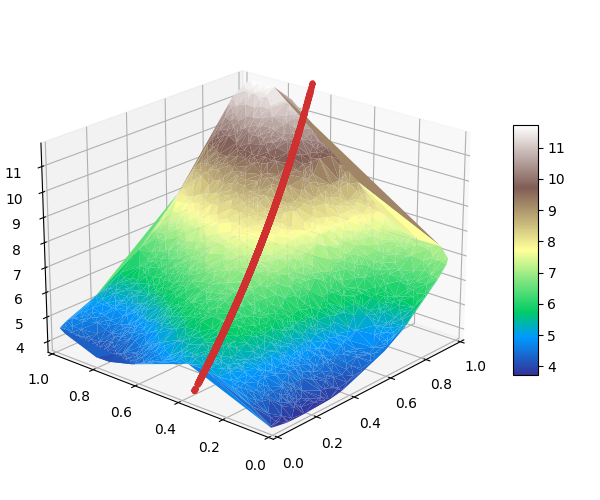
\includegraphics[width=.85\linewidth]{graphics/pipeline_current_1.png}
  \caption{Plot of the error function $e_0=f$ and its intersection with the first active subspace direction $v_1$ in \reddot}
\label{fig:pipeline_current_1}
\end{subfigure}%
\begin{subfigure}{.5\textwidth}
  \centering
  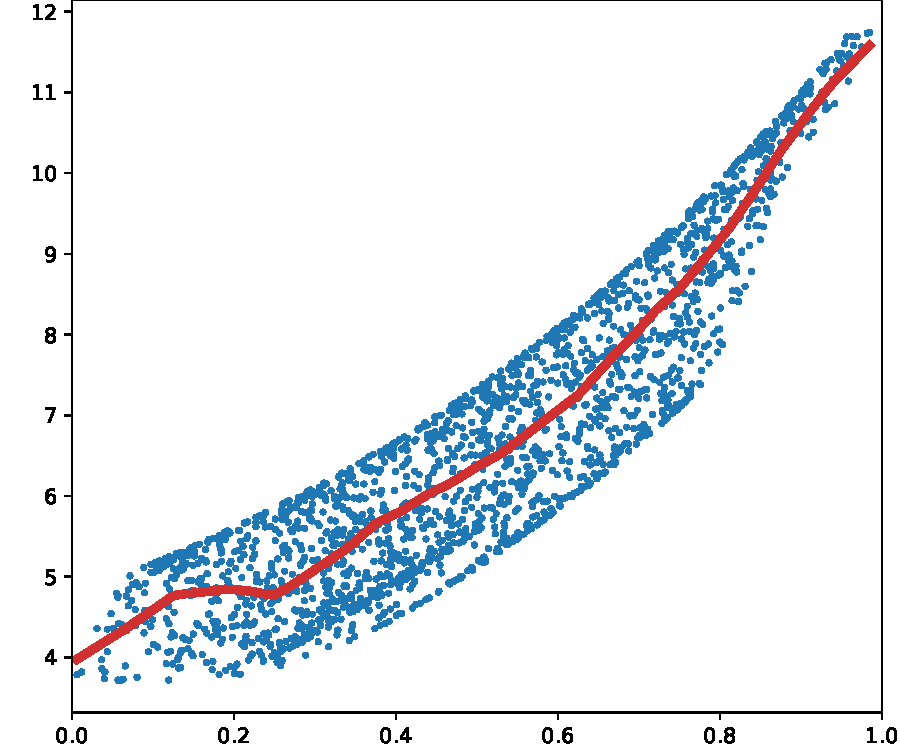
\includegraphics[width=.85\linewidth]{graphics/pipeline_local_1}
  \caption{Transformed input samples $S_t$ in \darkblue and the constructed surrogate $\hat{f}_1$ in \red.}
\label{fig:pipeline_local_1}
\end{subfigure}
\delimit
\caption{First iteration of the iterative transformation algorithm.}
\label{fig:pipeline_1}
\end{figure}
\end{mdframed}
%
As we can see in \cref{fig:pipeline_1}, the first algorithm iteration removes a big chunk of the original function $e_0=f$ to reduce the approximation error in the first step.
It identified the most active direction mostly right and was able to create a regression surrogate for the transformed function samples.
The regression surrogate had to employ a lot of regularization, as seen in\cref{fig:pipeline_local_1}, since there is still some function output contribution by the sinus term that will be projected onto the first active direction.

\begin{mdframed}[style=style]
\begin{figure}[H]
\begin{subfigure}{.5\textwidth}
  \centering
  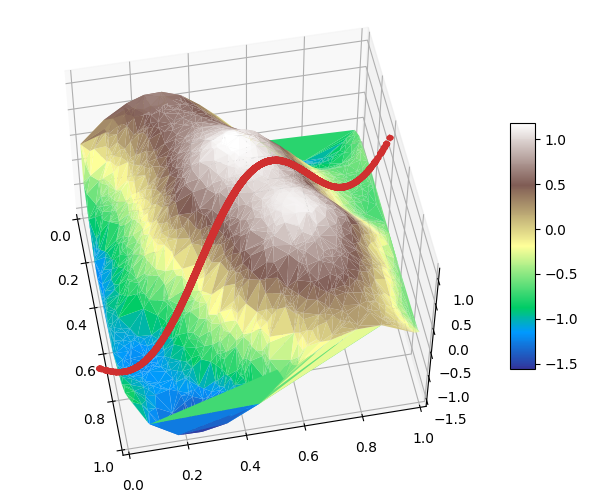
\includegraphics[width=.85\linewidth]{graphics/pipeline_current_2.png}
  \caption{Plot of the error function $e_1$ and its intersection with the first active subspace direction $v_1$ in \reddot}
\label{fig:pipeline_current_2}
\end{subfigure}%
\begin{subfigure}{.5\textwidth}
  \centering
  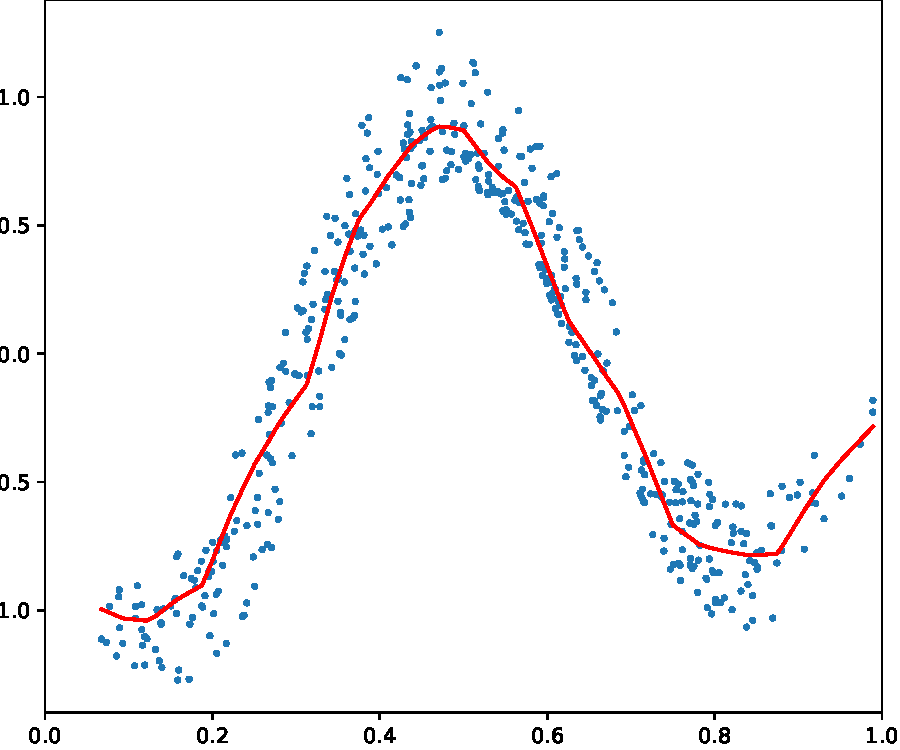
\includegraphics[width=.85\linewidth]{graphics/pipeline_local_2}
  \caption{Transformed input samples $S_t$ in \darkblue and the constructed surrogate $\hat{f}_2$ in \reddot}
\label{fig:pipeline_local_2}
\end{subfigure}
\delimit
\caption{Second iteration of the iterative transformation algorithm.}
\label{fig:pipeline_2}
\end{figure}
\end{mdframed}
%
In \cref{fig:pipeline_2}, we can clearly identify the remnants of the rotated sinus term that are the leftovers after the exponential term was mostly removed in the first iteration.
However, we can also see that the term is not completely the second term as there are a few small deviations.
In theory, an optimal method should be able to approximate $f$ without a resultung in a leftover error function after two iterations, as its compounded intrinsic dimension is $1$.
However, as the method is not perfect and encounters small errors from various sources throughout the algorithm, it can not approximate functions in an optimal way.
These are caused by inaccuracies inherent to the algorithm:
\begin{enumerate}
\item The active subspace method not finding suitable active directions, caused by the nature of the method itself
\item The gradient inputs for the active subspace method being biased, caused by using approximation methods
\item The regression method not producing ideal surrogates, caused by too little or too much regularization or insufficient samples at the boundaries as seen in \cref{fig:pipeline_local_1} on the left
\end{enumerate}

\begin{mdframed}[style=style]
\begin{figure}[H]
\begin{subfigure}{.5\textwidth}
  \centering
  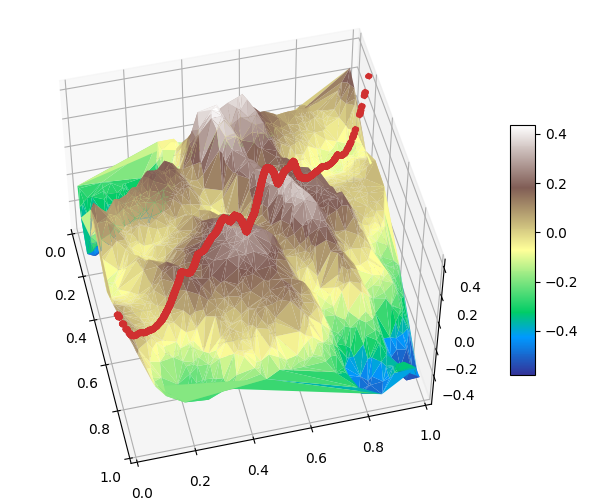
\includegraphics[width=.85\linewidth]{graphics/pipeline_current_3.png}
  \caption{Plot of the error function $e_3$ and its intersection with the first active subspace direction $v_1$ in \reddot}
\end{subfigure}%
\begin{subfigure}{.5\textwidth}
  \centering
  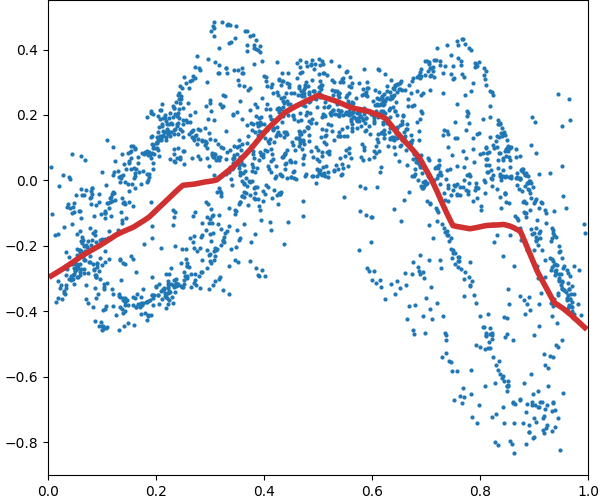
\includegraphics[width=.85\linewidth]{graphics/pipeline_local_3}
  \caption{Transformed input samples $S_t$ in \darkblue and the constructed surrogate $\hat{f}_3$ in \reddot}
\end{subfigure}
\delimit
\caption{Third iteration of the iterative transformation algorithm.}
\label{fig:pipeline_3}
\end{figure}
\end{mdframed}
%
As evident in \cref{fig:pipeline_3}, the algorithm hits a point where it can no longer effectively reduce the approximation error by adding another one dimensional surrogate, as the transformed input data is mostly two-dimensional noise that can't be regressed.
Even though, we can try to fit a heavily regularized surrogate to the transformed function samples, the gain is minimal.

\begin{mdframed}[style=style]
\begin{figure}[H]
\begin{subfigure}{.5\textwidth}
  \centering
  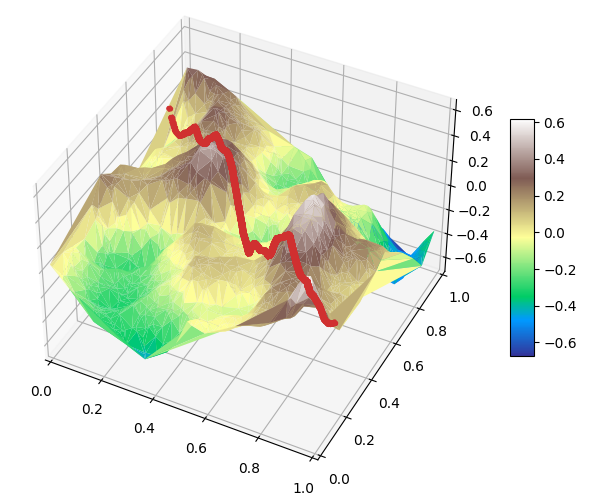
\includegraphics[width=.85\linewidth]{graphics/pipeline_current_4.png}
  \caption{Plot of the error function $e_4$ and its intersection with the first active subspace direction $v_4$ in \reddot}
\end{subfigure}%
\begin{subfigure}{.5\textwidth}
  \centering
  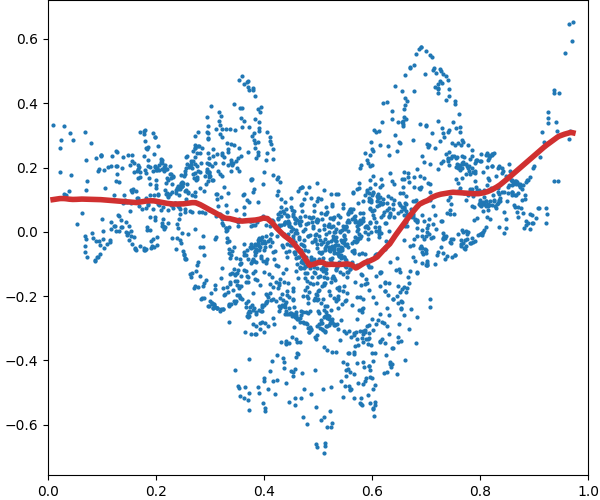
\includegraphics[width=.85\linewidth]{graphics/pipeline_local_4}
  \caption{Transformed input samples $S_t$ in \darkblue and the constructed surrogate $\hat{f}_4$ in \reddot}
\end{subfigure}
\delimit
\caption{Fourth iteration of the iterative transformation algorithm.}
\label{fig:pipeline_4}
\end{figure}
\end{mdframed}
%
In \cref{fig:pipeline_4}, we see that we definitely hit a convergent state as the change compared to the previous iteration is minimal again.
Therefore, the iteration stops there.

\section{Local vs global optimization}

The previously introduced transformation generation algorithm uses a local optimization approach to determine the optimal transformation to use.
However, in some cases this approach can lead the algorithm down a wrong path that will result in a worse approximation error than otherwise possible.

If we look at the example function from the previous section again and giving the algorithm the additional choice of not employing a lot of regularization, the algorithm might fall in to the trap of overfitting when only looking ahead one iteration:
\begin{mdframed}[style=style]
\begin{figure}[H]
\begin{subfigure}{.5\textwidth}
  \centering
  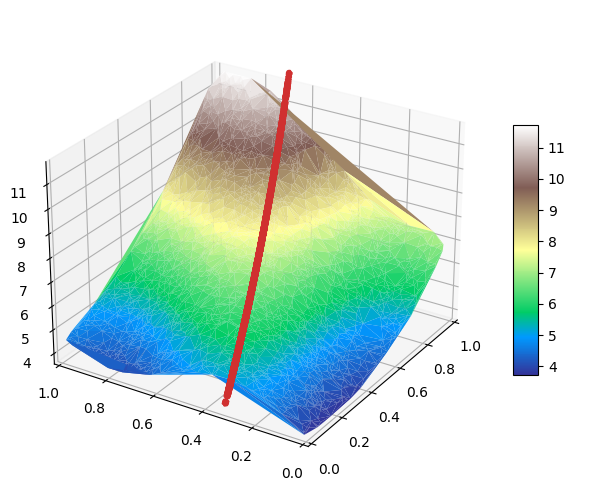
\includegraphics[width=.85\linewidth]{graphics/pipeline_bad_current_1.png}
  \caption{Plot of the error function $e_0=f$ and its intersection with the first active subspace direction $v_1$ in \reddot}
\label{fig:pipeline_bad_current_1}
\end{subfigure}%
\begin{subfigure}{.5\textwidth}
  \centering
  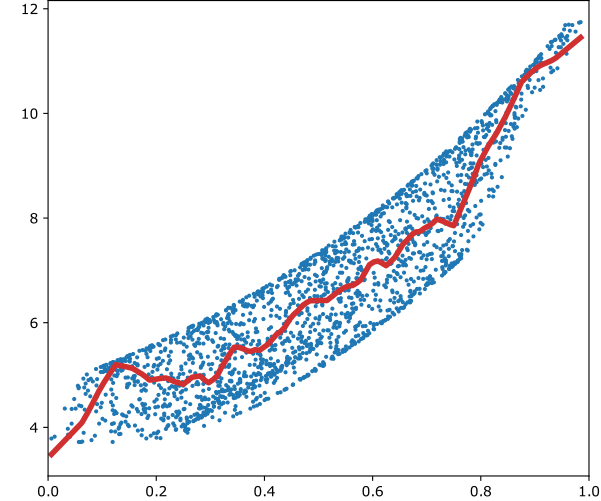
\includegraphics[width=.85\linewidth]{graphics/pipeline_bad_local_1}
  \caption{Transformed input samples $S_t$ in \darkblue and the constructed surrogate $\hat{f}_1$ in \red.}
\label{fig:pipeline_bad_local_1}
\end{subfigure}
\delimit
\caption{First iteration of the iterative transformation algorithm.}
\label{fig:pipeline_bad_1}
\end{figure}
\end{mdframed}
%
As we can see in \cref{fig:pipeline_bad_local_1}, the surrogate is overfitted.
While at this stage, the approximation error is almost equal to the more regularized surrogate from \cref{fig:pipeline_local_1}, this will propagate into the next iteration:

\begin{mdframed}[style=style]
\begin{figure}[H]
\begin{subfigure}{.5\textwidth}
  \centering
  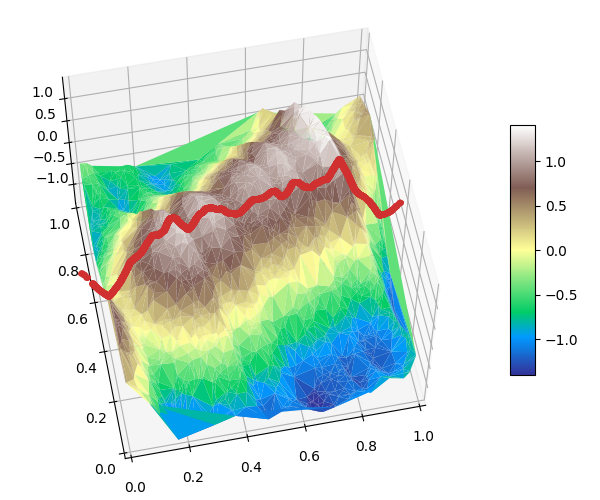
\includegraphics[width=.85\linewidth]{graphics/pipeline_bad_current_2.png}
  \caption{Plot of the error function $e_0=f$ and its intersection with the first active subspace direction $v_1$ in \reddot}
\label{fig:pipeline_bad_current_2}
\end{subfigure}%
\begin{subfigure}{.5\textwidth}
  \centering
  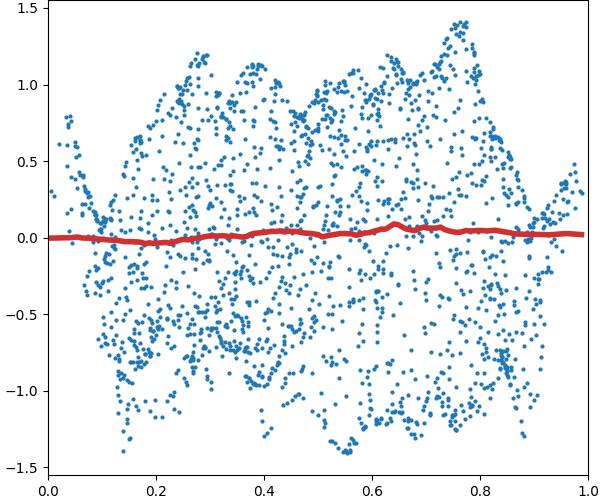
\includegraphics[width=.85\linewidth]{graphics/pipeline_bad_local_2.png}
  \caption{Transformed input samples $S_t$ in \darkblue and the constructed surrogate $\hat{f}_1$ in \red.}
\label{fig:pipeline_bad_local_2}
\end{subfigure}
\delimit
\caption{First iteration of the iterative transformation algorithm.}
\label{fig:pipeline_bad_2}
\end{figure}
\end{mdframed}
%
\Cref{fig:pipeline_bad_local_2} shows that no effective surrogate can be created as the input data is mostly just noise, because the surrogate in the previous iteration was overfitted.
A solution would be to instead look ahead more than iteration in cases where overfitting is possible:

\begin{mdframed}[style=algstyle,frametitle={\textbf{function} \texttt{generateBestTransformationLookAhead}{$(e, r_{\text{min}} ,r_{\text{max}}, i)$}}]
\normalsize
\vspace{5.5mm}
\begin{algorithmic}[1]
    \State $t^\ast \gets \mathds{1}$
    \State $\varepsilon_{min} \gets \infty$
    \For{$r = r_{\text{min}},\dots,r_{\text{max}}$}
      \State $t_r$ $\gets$ \texttt{generateTransformation}(e, r)
      \State $\hat{f}_{c^\ast}^l$ $\gets$ \texttt{transformedSurrogateSum}$(f, i)$
    	\State $\varepsilon \gets \varepsilon(\hat{f}_c^l)$
    	\If{$\varepsilon < \varepsilon_{min}$}
    	  \State $\varepsilon_{min}\gets \varepsilon$
    	\State $t^\ast \gets t_r$
    	\EndIf
    \EndFor
    \State \Return{$t^\ast$}
\end{algorithmic}
\vspace{-1.5mm}
\delimit
	\captionof{algorithm}{Pseudocode of the transformation generation algorithm. Parameters are the current error function $e$, the minimum reduced dimension $r_{\text{min}}$, maximum reduced dimension $r_{\text{max}}$, and the amount of look ahead iterations $i$.}
	\label{alg:lookahead}
\end{mdframed}
%
\Cref{alg:lookahead} is very similar to \cref{alg:besttrans}, with the only difference being the way how a newly generated transformation is evaluated.
Instead of effectively performing only one look ahead iteration, we perform $i$ look ahead iterations to better gauge the quality of the produced transformation with regards to the resulting approximation error of the surrogate sum.
To guarantee fast execution speed, we use lo-fi surrogates when looking ahead.
Of course the actual implementation of \texttt{transformedSurrogateSum} when called from \texttt{generateBestTransformationLookAhead} can not also make use of the multiple iteration look ahead approach internally to prevent infinite loops.

\chapter{Implementation}
\label{chap:c6}

This chapter will cover the practical implementation of the iterative algorithm of \cref{chap:c5}.
We model the general structure of various parts of the implementation as components and use component diagrams to described their general internal structure and possible configuration parameters.
The notation of these component diagrams is shown in \cref{fig:defs}.
This surface level description of the whole implementation will make the evaluation results presented later as transparent as possible, as it will list and explain possible algorithm configuration parameters that will impact the end result.

\begin{mdframed}[style=style,frametitle={Notation}]
\begin{figure}[H]

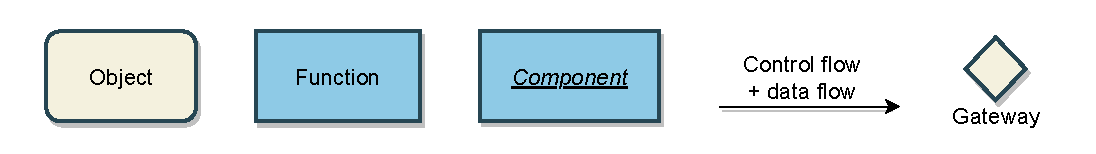
\includegraphics[width=\textwidth]{graphics/definitions.pdf}
\vspace{-7.5mm}

\delimit

\vspace{3.5mm}

\begin{description}
\item[Elements] {~ \begin{itemize}[\null]
\item \textbf{Object}: An object can represent any kind of data, for example a model function, a function sample, a transformation function, a surrogate, and more.
\item \textbf{Function}: A function takes optional inputs in the form of objects, performs some kind of operation, and outputs an object.
\item \textbf{Function component}: A function component is a also function, where the actual implementation can be exchanged for many different function implementations of the same interface.
\item \textbf{Control flow + data flow}: Arrows signal control flow and also data flow if an object is shown.
\item \textbf{Gateway}: A gateway evaluates an attached condition and decides which outgoing control flow to follow.
\end{itemize}}
\end{description}

\delimit

\captionof{figure}{Notation used for different elements in the component structure diagrams in this chapter.}
\label{fig:defs}
\end{figure}
\end{mdframed}


\newpage
\section{Transformation pipeline}
\label{sec:tp}

The complete transformation process is modeled and implemented as an iterative pipeline that is made up of different components to allow for maximum flexibility.
Every pipeline iteration has the goal of adding another transformed surrogate to the current sum of surrogates to further improve the approximation.
Many pipeline components can be exchanged for many different implementation types, where instances of these types can also be customized by passing configuration parameters.
The pipeline structure is visualized in figure \cref{fig:tp}.

\begin{mdframed}[style=style,frametitle={Transformation Pipeline}]
\begin{figure}[H]

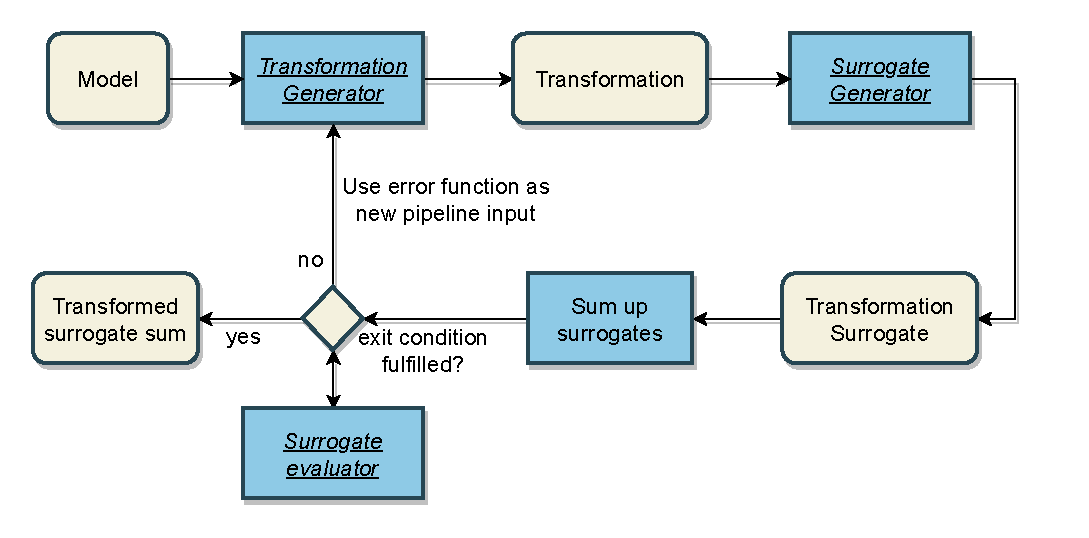
\includegraphics[width=\textwidth]{graphics/TransformationPipeline.pdf}
\vspace{-7.5mm}

\delimit

\begin{description}
\item[Parameters] {~ \begin{itemize}[\indent{}]
\item \texttt{\textbf{exitCondition}}: A predicate indicating whether the pipeline iteration loop should exit. This can be using a variety of conditions such as a maximum iteration count or a maximum approximation error.
\item \texttt{\textbf{sampleCount}}: The amount of function samples $n$ used during pipeline execution. These samples are used for a variety of operations and split into train, validate, and test datasets in each iteration.
\end{itemize}}
\end{description}

\delimit

\captionof{figure}{Component structure of the transformation pipeline and its associated possible configuration parameters.}
\label{fig:tp}
\end{figure}
\end{mdframed}

The most important component of the transformation pipeline wrt. achieving good approximation results is the transformation generator \cref{sec:tg}, as the quality of a transformation will be passed down the line in each iteration.
The generated transformation is then fed into a surrogate generator \cref{sec:sg}, which will generate the transformed surrogate.
Note that in the abstract pipeline, any type of surrogate like sparse grids and RBFs can be generated in theory.
The newly generated surrogate is then added to the sum of previously generated surrogates to obtain the new transformed surrogate sum.
At the end of each iteration, we decide whether to exit the pipeline or continue.


\newpage
\section {Transformation generators}
\label{sec:tg}

The transformation generator component has the responsibility of finding a good transformation function to use for a pipeline iteration.
We covered the creation of input transformation extensively in chapter \cref{chap:c4}, and transformation generators are a straightforward implementation of the covered methods, with the goal to provide a uniform interface.

\subsection {Transformation stream generator}
\label{sec:tsg}

We saw previsouly that we can generate a whole family of transformations for every calculated active subspace matrix or random orthogonal basis, which is usually accomplished by using different values for the reduced dimension $r$, i.e. cutting less or more dimensions off.
To apply this concept and to couple it with other components introduced later on, such as transformation evaluators, this implementation makes use of so-called transformation stream generators.

\begin{mdframed}[style=style,frametitle={Transformation generator (stream-based)}]
\begin{figure}[H]
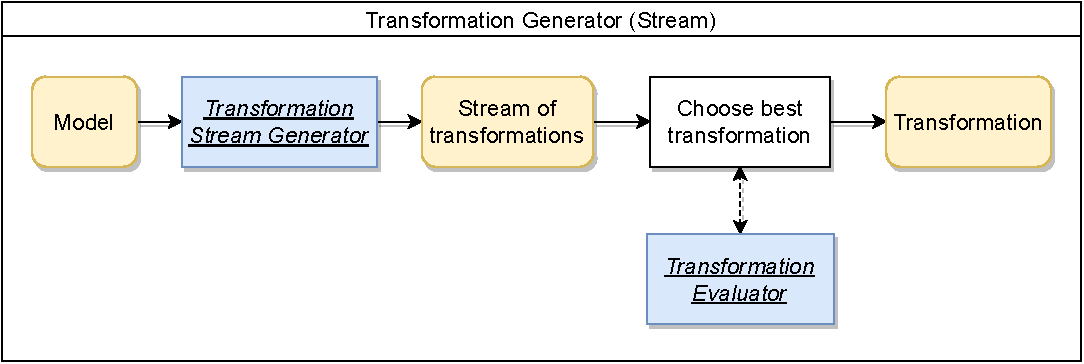
\includegraphics[width=\textwidth]{graphics/TransformationGen_Stream.pdf}
\delimit

\captionof{figure}{Component structure of a stream-based transformation generator.}
\end{figure}
\end{mdframed}

A transformation stream generator will generate as much different transformations as it can, where the range of possible transformations is defined by multiple parameters.
Every transformation that is generated from the stream is evaluated using a transformation evaluator and the best transformation will be chosen and returned in the end.

\newpage

\subsection{Active Subpsace stream generator}

Transformation generation with the active subspace method as covered in \cref{sec:as} is implemented as a transformation stream generator component, since there are multiple different cutoff possibilities with $r$.
The exact range of the cutoff dimensions can be customized using various parameters as seen in figure \cref{fig:astsg}.

\begin{mdframed}[style=style,frametitle={Transformation stream generator (active subspaces)}]
\begin{figure}[H]
\vspace{5px}
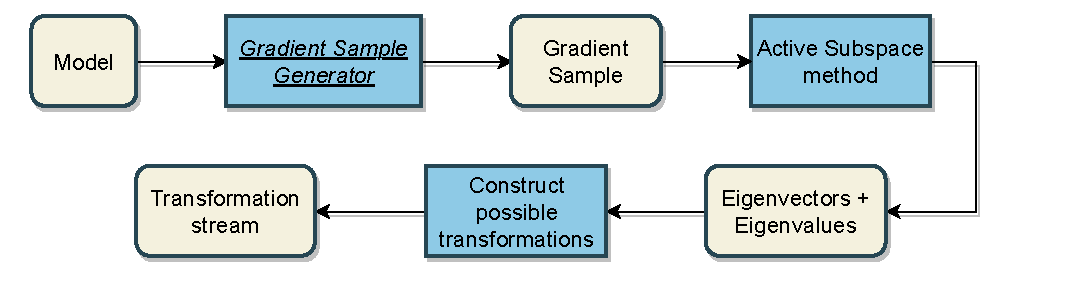
\includegraphics[width=\textwidth]{graphics/TransformationStreamGen_AS.pdf}

\delimit

\begin{description}
\item[Parameters] {~ \begin{itemize}[\indent{}]
\item \texttt{\textbf{maxSampleCount}}: The maximum amount of samples used to create a gradient sample.
\item \texttt{\textbf{minDimensions}}: The minimum amount of used eigenvectors, i.e. the lower bound for $r$.
\item \texttt{\textbf{maxDimensions}}: The maximum amount of used eigenvectors, i.e. the upper bound for $r$.
\item \texttt{\textbf{minEigenValueShare (= 0)}}: Imposes a lower bound on the possible values of $r$ by requiring that it holds that $\sum_{i=1}^r \lambda_i / \sum_{i=1}^d \lambda_i \geq \texttt{minEigenValueShare}$.
\end{itemize}}
\end{description}
\delimit
\captionof{figure}{Component structure of an active subspace transformation stream generator and the associated possible configuration parameters.}
\label{fig:astsg}
\end{figure}
\end{mdframed}

Setting a \texttt{minEigenValueShare} value allows us to flexibly adjust the upper bound of $r$ such that we do not consider the last few eigenvectors with way smaller eigenvalues compared to the first few.
A common values used is $\texttt{minEigenValueShare=0.95}$.

The Monte-Carlo based active subspace method requires gradient samples as inputs.
These are generated by a gradient sample generator component.
Possible implementations for gradient computation that we already covered in section \cref{sec:as} are available to choose from, as seen in \cref{fig:gg}.


\newpage

\begin{mdframed}[style=style,frametitle={Gradient sample generator}]
\begin{figure}[H]
\begin{description}
\item[\texttt{\textbf{givenGradient()}}:] If the gradient function of the model function $f$ is known or easy to calculate analytically, then generating a gradient sample is straightforward by just evaluating the gradient function at the sample points.
\item[\texttt{\textbf{finiteDifferences($h$)}}:] Alternatively, the sample gradients can be determined using finite differences if the runtime cost of $d$ model function evaluations per sample point is acceptable.
\item[\texttt{\textbf{randomNeighbour($n'$)}}] Random neighbour approximation.
\item[\texttt{\textbf{nearestNeighbour($n', m$)}}] Nearest neighbour approximation.
\end{description}
\delimit
\captionof{figure}{List of available gradient sample generator implementations.}
\label{fig:gg}
\end{figure}
\end{mdframed}

\subsection {Random stream generator}
\label{sec:rtg}

An alternative approach to finding a transformation function is just generating a random orthonormal basis, as covered in \cref{sec:rt}.
This random transformation generator is easy to implement, as shown in \cref{fig:rtsg}, can generate new transformation functions almost instantly and offers a purely exploratory approach to finding the best transformation.

\begin{mdframed}[style=style,frametitle={Transformation stream generator (random)}]
\begin{figure}[H]

\vspace{5px}
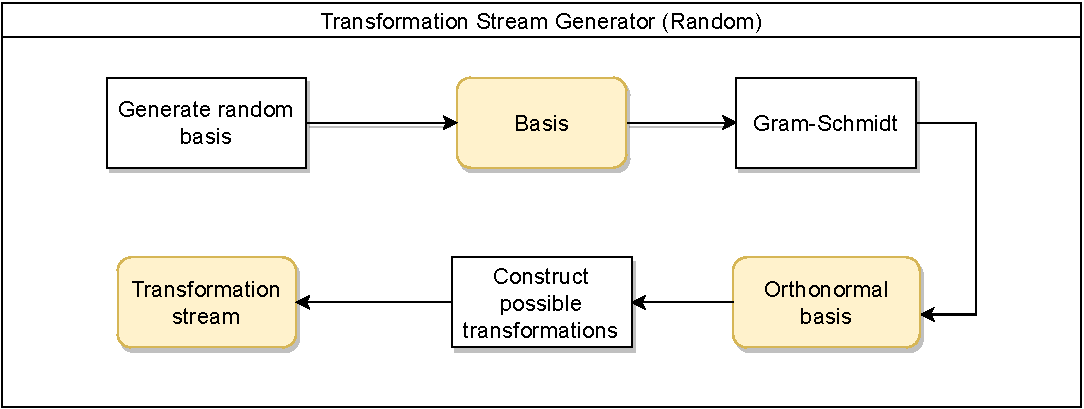
\includegraphics[width=\textwidth]{graphics/TransformationStreamGen_Random.pdf}

\delimit
\begin{description}
\item[Parameters] {~ \begin{itemize}[\indent{}]
\item \texttt{\textbf{minDimensions}}: The minimum amount of used basis vectors, i.e. the lower bound for $r$.
\item \texttt{\textbf{maxDimensions}}: The maximum amount of used basis vectors, i.e. the upper bound for $r$.
\end{itemize}}
\end{description}
\delimit
\captionof{figure}{Component structure of an random transformation stream generator and the associated possible configuration paremeters.}
\label{fig:rtsg}
\end{figure}
\end{mdframed}

\newpage

\subsection {Iterative transformation generator}

In some cases, especially when dealing with a random transformation generation as shown in \cref{sec:rtg}, the probability of finding a good transformation in one try is very low, it makes sense to also introduce an iterative transformation generator component, which can be combined with any other transformation generator component, e.g. a stream-based one.
It can also be used with the active subspace transformation generator to try to find the best transformation out of several active subspace calculations with different input samples.

\begin{mdframed}[style=style,frametitle={Transformation generator (iterative)}]
\begin{figure}[H]
	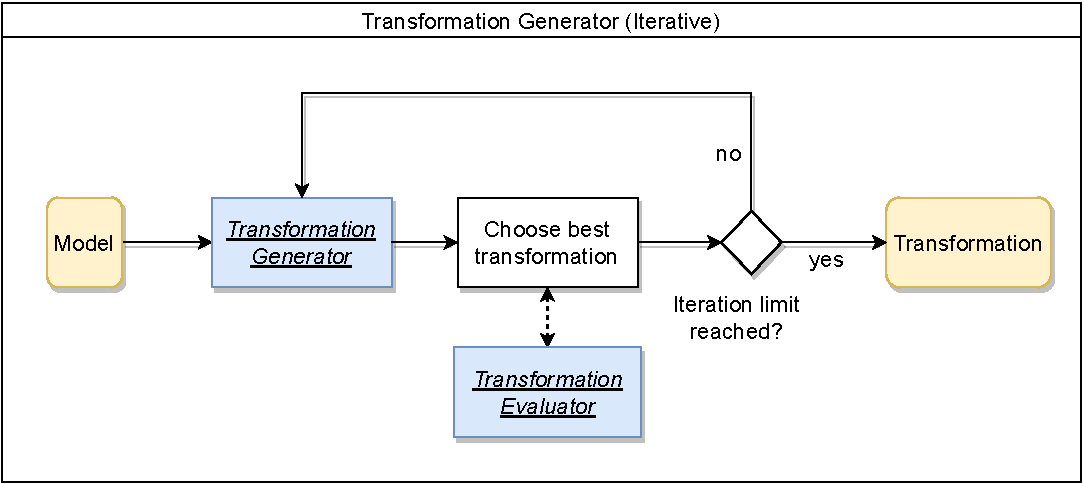
\includegraphics[width=\textwidth]{graphics/TransformationGen_Iterative.pdf}

\delimit

\begin{description}
\item[Parameters] {~ \begin{itemize}[\null]
\item \texttt{\textbf{numIterations}}: The amount of iterations that should be executed.
\end{itemize}}
\end{description}

\delimit
\captionof{figure}{Component structure of an iterative transformation generator and the associated possible configuration parameters.}
\label{fig:itg}
\end{figure}
\end{mdframed}


Note that this iterative approach is independent from the pipeline iterations, i.e. an iterative transformation generator executes all of its iterations during one pipeline step to determine the best transformation to be used in the one pipeline step.
To achieve fast execution of many iterations, we choose to work on lo-fi surrogates during the iterations when interacting with transformation evaluator.
This means that the approximation errors used to identify the best transformation do not necessarily come close to the actual hi-fi approximation errors.
\Cref{sec:lofi} touched upon the required considerations when employing multifidelity simulations.

\newpage
\section {Evaluators}

\subsection {Surrogate evaluator}
\label{sec:se}

The role of a transformation evaluator is to take a newly constructed transformation $t(x)$, evaluate its quality and make it comparable to other transformations.
This is used for iterative and stream-based transformation generators and by the pipeline.
While this is a pretty straightforward process, it can still be customized by changing the surrogate construction rules and error metric.

\begin{mdframed}[style=style,frametitle={Surrogate evaluator}]
\begin{figure}[H]
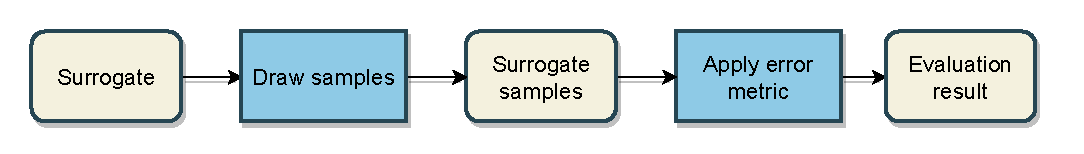
\includegraphics[width=\textwidth]{graphics/SurrogateEval.pdf}
\vspace{-4.5mm}

\delimit

\begin{description}
\item[Parameters] {~ \begin{itemize}[\indent{}]
\item \texttt{\textbf{errorMetric}}: The amount of iterations that should be executed.
\end{itemize}}
\end{description}

\delimit

\captionof{figure}{Component structure of a surrogate evaluator and the associated possible configuration parameters.}
\label{fig:se}
\end{figure}
\end{mdframed}

Common error metrics used in this thesis include MSE, RMSE, and NRMSE.
If we want to steer the transformation generation process into a certain direction, like preferring lower-dimensional transformations, we can introduce a few modifications, such as a penalty term that grows with the amount of reduced dimensions of the transformation.

\subsection {Transformation evaluator}
\label{sec:te}

The role of a transformation evaluator is to take a newly constructed transformation and evaluate its quality by assigning it a certain value to make it comparable to other transformations.
As mentioned in \cref{sec:te}, evaluating the true quality of a transformation is only really possible by creating a surrogate from it.
We therefore first generate a surrogate with a surrogate generator \cref{sec:sg} and then make use of a surrogate evaluator \cref{sec:se} to return the evaluation result.
While this is a pretty straightforward process, it can still be customized by changing the surrogate construction rules, for example by using a lofi surrogate generator to speed up the evaluation.

\newpage
\begin{mdframed}[style=style,frametitle={Transformation evaluator (forward looking)}]
\begin{figure}[H]
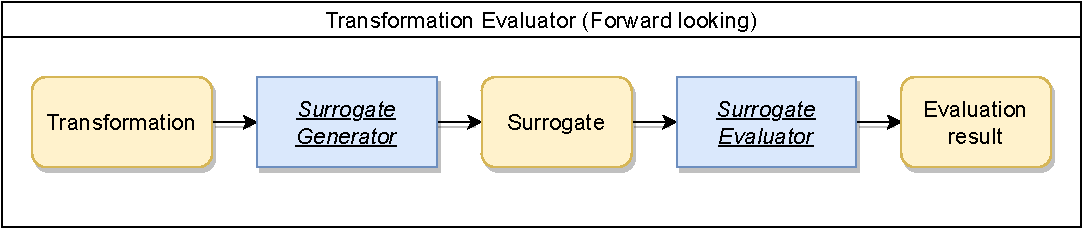
\includegraphics[width=\textwidth]{graphics/TransformationEval.pdf}
\delimit

\captionof{figure}{Component structure of a forward looking transformation evaluator.}
\label{fig:te}
\end{figure}
\end{mdframed}

\section {Surrogate generators}
\label{sec:sg}

The last component needed for the pipeline implementation are surrogate generators, which construct the function $\hat{f}_t$ for given configuration parameters and the transformed input samples
\begin{equation}
S_t=\{(t(x_1), f(x_1), \dots, (t(x_n), f(x_n))\} \subseteq T \times \mathds{R}
\end{equation}
Their implementation is straightforward, as the construction of sparse grid surrogates and also RBF surrogates was covered in detail and the surrogate generators closely match that.


\subsection {Sparse Grid surrogate generator}

The sparse grid generation implementation is realized with SGpp \cite{Pflueger2010} library.
In the case of Sparse Grid surrogates, as used in this thesis, the construction parameters contain all the normally required inputs like grid type, basis type, adaptivity properties, and regression parameters.
Some sparse grid parameters, like the level, also have to be adapted to handle arbitrary surrogate dimension, as a surrogate generator should be decoupled from the used dimension $r$. 
This means that instead of passing a fixed level $\ell$ as a parameter, we instead use \texttt{approxGridPoints} to specify how much grid points the surrogate should approximately have and determine the approapriate level from there as it varies greatly for different values of $r$.
Furthermore, for sparse grid regression we similarly express the amount of training samples with the variable \texttt{trainSamplesPerGridPoint}, to automatically link the amount of grid points and used training samples together.

\subsection {RBF surrogate generator}

Radial basis function surrogates are implemented with the help of ALGLIB \cite{Bochkanov}, a numerical analysis and data processing library which supports fitting RBFs on arbitrary input data.
Compared to sparse grids, RBFs do not have a lot of configuration parameters.
The main parameters are the shape parameter $\epsilon$ and also a regularization factor $\lambda$.
RBF surrogates can be created with the interpolation approach, as they can interpolate from arbitrary function samples $S_t$.

\section{Example pipeline}

To give an example on how an actual transformation pipeline instance could look like, we will construct a simple one here.
As many components are designed in a way to be forward looking, we can think of the transformation pipeline as a collection of different subpipelines.
The high fidelity subpipeline is responsible for finding the the best and most expensive possible hi-fi surrogate for each iteration.
It does so by usually evaluating the quality of multiple transformations from one family of possible transformations, such as the computed active subspaces $W$, using a look-ahead approach, i.e. executing a low fidedily subpipeline that evaluates the transformation quality by effectively performing a whole iteration with lower fidelity surrogates.
This lo-fi subpipeline has to be quick to execute, as it is runs multiple times for all possible values of $r$.
The structure of an example pipeline can be seen in \cref{fig:tpex}.

\begin{mdframed}[style=style]
\begin{figure}[H]
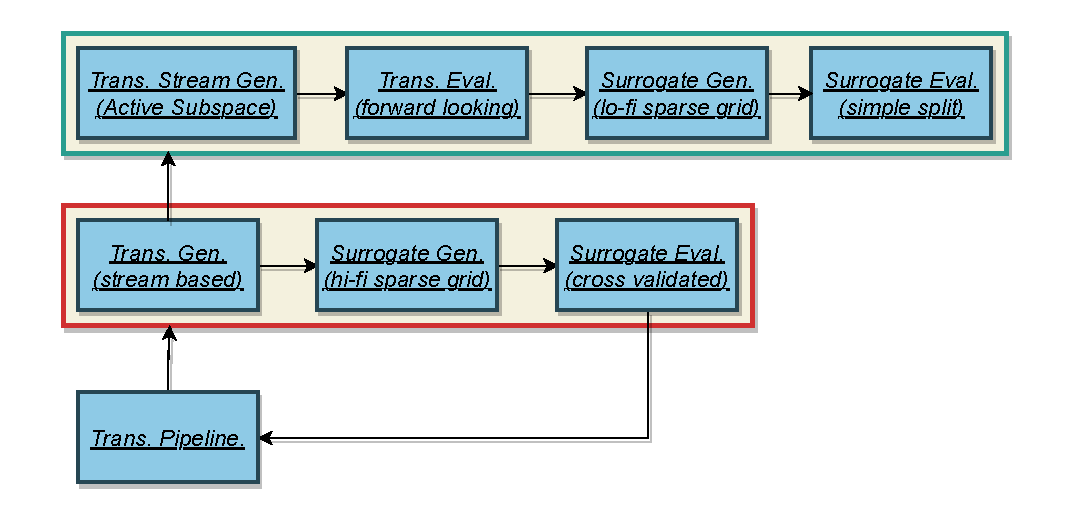
\includegraphics[width=\textwidth]{graphics/PipelineExample.pdf}
\delimit

\captionof{figure}{Structure and control flow of an examplary transformation pipeline.\\
The \red box identifies the hi-fi subpipeline components, and the \green box identifies the lo-fi subpipeline components.}
\label{fig:tpex}
\end{figure}
\end{mdframed}


\section{Sample budgeting}

A central aspect of the transformation is pipeline is the handling of input samples
\begin{equation}
S_t=\left\{(t(x_i), f(x_i))\right\}_{i=1}^n,
\nonumber
\end{equation}
as they are used in almost every pipeline component.
With the heavy use of the same samples across various stages, special care has to be taken to prevent overfitting.
For example, the transformation generator, surrogate generator, and surrogate evaluator should all work with different samples such that no overtting can possibly take place.

Also, components that only work together, such as the surrogate generator and surrogate evaluator, are designed to coordinate their sample use with each other.
For example, a cross validated surrogate evaluator partitions the input samples multiple times and each time passes the train partition to the surrogate generator to generate a surrogate and then evaluates the quality using the associated validate partition.
Therefore, the actual implementation control flow is not as simple as shown in \cref{fig:tpex}.
The sample subset, that is passed down by each component to the next ones is also shuffled, such that partioning them into train and validation samples is not deterministic when performing multiple pipeline iterations with the sample input samples.

The pipeline works for any amount of input samples, as long there is at least a minimum viable amount, and does not require any additional function evaluations to work efficiently, which makes it very flexible.
This is an advantage compared to any interpolation based approaches.

\chapter{Experiments}
\label{chap:c7}

The construction process for transformed surrogates is realized through the transformation pipeline, which consists out of many different components.
These components interact with each other and pass data down the transformation pipeline, which can cause compounding inaccuries and errors if the inputs from a previous stage are inaccurate.
In this evaluation chapter, we investigate the qualities and properties of transformation pipeline components in an isolated environment before performing experiments on real world model functions in the next chapter.
For this purpose, we first look at the low-dimensional Ishigami function followed by the higher-dimensional wing weight function.

\section{Ishigami function}

We start off with the low dimensional Ishigami function \cite{Ishigami1990AnIQ}:
\begin{equation}
f(x)=\sin(x_1) + a \sin^2(x_2) + b x_3^4 \sin(x_1), ~~ a = 7, b=0.1
\end{equation}
%
The function originally has been used for uncertainty quantification purposes, but has also been used to test sensitivity analysis techniques \cite{Sobol1999}.
To get an idea of the general structure and importance of the inputs, we apply the active subspace method on this function, which yields the following results:

\begin{mdframed}[style=style]
\begin{figure}[H]
\centering

\bgroup
\def\arraystretch{1.2}% 
  \begin{tabular}{ l | c c c}
$i$ & $v_i$ & $\lambda_i$ & $\lambda_i / \sum_{i=1}^d \lambda_i$\\
\hline
$1$ & $(+0.005, ~+0.999, ~+0.007)^T$ & 967.93 & $81.7\%$\\
$2$  & $(+0.540, ~+0.003, ~-0.841)^T$ & 112.20 & $9.5\%$\\
$3$ & $(-0.841, ~+0.008, ~+0.540)^T$ & 104.77 & $8.8\%$\\
\end{tabular}
\egroup
\vspace{0.5em}

\delimit

\captionof{table}{Computed eigen vectors, eigen values, and eigen value shares of the active subspaces for the Ishigami function using the Monte-Carlo method and $10^6$ samples.}
\label{tab:ishigami_as}
\end{figure}
\end{mdframed}
%
Based off the values in \cref{tab:ishigami_as}, we can see that the most active direction almost exactly corresponds to second input dimension, and is reponsible for a big chunk of the average gradient change, while the other two active directions are less important and also not axis aligned.
These two less active directions are however not neglible, as their combined eigen value share still is $18.3\%$.

As we will make use of lo-fi and hi-fi simulations, we will distinguish the resulting errors by denoting them by $\varepsilon^\mathrm{l}_{\mathrm{NRMSE}}$ and $\varepsilon^\mathrm{h}_{\mathrm{NRMSE}}$ respectively.
For the Ishigami function in the lo-fi case, we use a sparse grid surrogate generator with a modified linear basis, no refinments, and a value of \texttt{approxGridPoints}$=250$.
For the hi-fi case, we use a sparse grid surrogate generator with $10$ refinments, 10 refined grid points per refinement, and a value of \texttt{approxGridPoints}$=1000$.
These configurations will ensure lo-fi surrogates that are fast to evaluate and hi-fi surrogates that have a sufficient amount of accuracy when performing a lot of pipeline iterations in this chapter.

\subsection{Orientation changes}

While the main focus lies on dimension reducing transformations with $r < d$, we still take a short look at the quality of simple dimension preserving linear transformations with $r=d$, which are effectively only changing the orientation of the function inputs.
For the orientation change, we use all computed active subspace directions from \cref{tab:ishigami_as}, or in other words apply the transformation $t_{W_3}$ on the inputs.
As we discussed in \cref{sec:ms}, with a few small modifications concerning model function evaluations outside of $\Omega$, we can also apply the interpolation method to construct a transformed sparse grid surrogate.
In this section, we are interested in answering the following questions:
\begin{enumerate}
\item How does the approximation error compare when applying an orientation changing transformation with $r=d$?
\item How big is the approximation error difference between interpolation and regression surrogates?
\item How is the approximation error affected when transformations and regression are used together?
\item How much difference is there between normal sparse grids and boundary grids?
\end{enumerate}
%
Compared the non transformed interpolation approach, the approximation error should be improved by the more optimal alignment of inputs.
On the other side, the unused parts of surrogate space (see \cref{sec:tis}) effectively reduce the resolution of the sparse grid surrogate and may make some grid points obsolete.
Furthermore, the necessary model function evaluations outside of $\Omega$ might worsen the approximation quality if they deviate sharply from function values inside $\Omega$ and might create steep value differences at the boundaries of $T$.

\begin{mdframed}[style=style]
\begin{figure}[H]
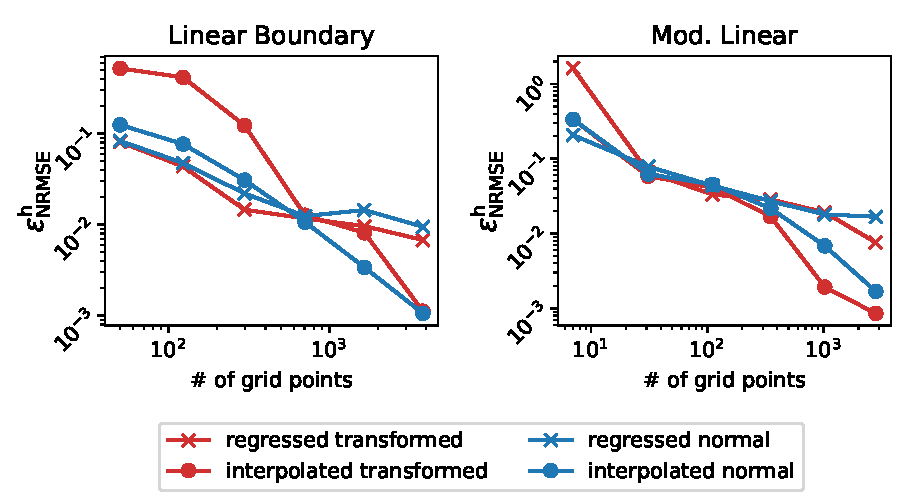
\includegraphics[width=\textwidth]{graphics/ishigami_orientation}
\delimit

\captionof{figure}{Approximation errors of transformed and untransformed sparse grid surrogates for the Ishigami function with linear boundary and modified linear basis types. The transformation is constructed with active subspaces and the finite differences method.}
\label{fig:ishigami_errors}
\end{figure}
\end{mdframed}
%
As we can see in \cref{fig:ishigami_errors}, the pure orientation change does not lead to better interpolation results.
In this concrete example, the penalty of the unused transformation space $U_t$ evens out the gains from a more optimal orientation for sparse grid surrogates.
As we do not perform a dimensionality reduction in this example, even if it would be feasible, this results in a constructed surrogate space that covers way more than the transformation space.
In this case the value is $\tilde{u}_t=0.44$, which means that $T$ only makes up $56\%$ of the surrogate space $S$ and the grid resolution is effectively lower and some grid points may be unused.
Furthermore, the introduced regression penalty, compared to the interpolation method, is factor of approximately $10^1$.
There are no significant quality differences when using modified linear basis functions instead of a linear basis with boundaries, which is why we will continue to use a modified basis for the Ishigami function for the rest of this section, as they require less grid points.

Based on these results we can conclude that, even though there is no improvement with this method, there is also no significant downside, even as $\tilde{u}$ is large and regression is used.
This can be seen as a positive insight, as it means that having a lot of unused space, which is not to avoid when using linear transformations, approximately cancels out with the orientation improvements.
Also, the additional use of regression only results in a slight increase of the approximation error.
As the tansformation process focuses on dimension reducing linear transformations that have to deal with unused space and can only use regression, this means that the individual transformed sparse grid surrogates do not become worse just through the orientation change, but allow for a much more flexible dimension reduction process.
Therefore, dimensionality reducing transformations seem to have a much bigger potential.

\subsection{Dimensionality reducing transformations}

Next, we look at dimensionality reducing transformations with $r < d$.
Note that for this low-dimensional model function, there is no real need to perform a dimensionality reduction, as the curse of dimensionality does not affect sparse grid surrogates heavily for $d=3$.
We can therefore not expect to see any gain from applying a transformation with $r < d$, as this will only happen for higher dimensions.
Even though reducing transformations should not be able to compete with normal interpolation, we are still interested in answering some basic questions:
\begin{enumerate}
\item By how much does dimensionality reduction increase the approximation error?
\item How much do the increased approximation errors correlate with the computed active subspace eigen values?
\end{enumerate}
%
Based off the active subspace information from \cref{tab:ishigami_as}, a one-dimensional reduction by cutting off the eigen vectors $v_2$ and $v_3$ looks feasible, as the first active direction covers the majority of the eigen value share.
However, as already discussed in \cref{sec:asl}, the active subspace method can be biased and also not return active directions that are suited for the transformation process.
Therefore, the primarily used pipeline component uses a look ahead approach to evaluate the suitability of the computed active directions and corresponding eigen values, instead of relying solely on the active subspaces results.

To better investigate the active subspace properties, we generate transformations for $r=1$ and $r=2$.
Since these are dimensionality reducing transformations, we can only create regression surrogates.
\begin{mdframed}[style=style]
\begin{figure}[H]
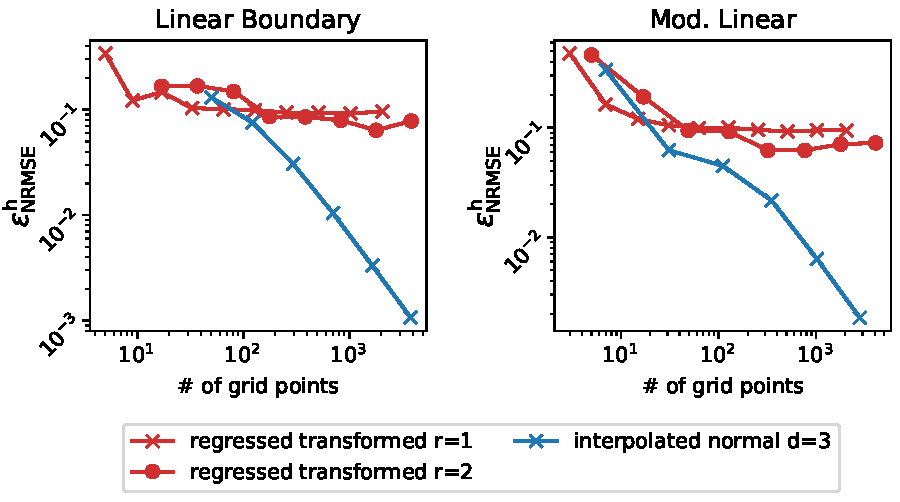
\includegraphics[width=\textwidth]{graphics/ishigami_red}
\delimit

\captionof{figure}{Approximation errors of reduced sparse grid surrogates for the Ishigami function with linear boundary and modified linear basis types. A normal interpolated sparse grid surrogate is also included for comparision.}
\label{fig:ishigami_red}
\end{figure}
\end{mdframed}
%
As we can see in \cref{fig:ishigami_red}, the dimensionality reducing transformations leads to, as expected, way worse results and does not provide usable surrogates.
We see that the approximation error for the reduced surrogates hits the convergent state very fast and an increase in grid points does not improve the surrogate quality.
Furthermore, the actual approximation error of the reduced surrogates does not correlate with the active subspace eigen values.
Even though the eigen value share of the first two eigen vectors is around $90\%$, the loss of the approximation quality when cutting of the most inactive eigen vector in the $r=2$ case is very large.

\subsection{Active subspace approximations}

Another central aspect of the transformation pipeline is the quality of the generated transformations for any given value for $r$.
In cases the transformation is constructed using the active subspace method, we are interested in the quality differences between the available active subspace approximation methods (see \cref{sec:as_est}), and want to ideally make use of the neighbour approximation methods, as they don't require known gradients and no additional model function evaluations.
We are interested in answering the following questions:
\begin{enumerate}
\item How much do the approximated active subspaces differ from the true active subspaces?
\item Do the active subspace differences actually manifest themselves in the approximation error?
\item Which approximation method performs the best?
\end{enumerate}
%
To judge the quality of approximated gradients, we first have to define an error metric for them:
\begin{definition}[Gradient approximation error]
Let $S=\{(x_i, f(x_i)\}_{i=1}^n$ be a set of samples, and let $\widetilde{\nabla} f(x_i)$ the approximated gradient for each sample point $x_i$. We then define
\begin{equation}
\varepsilon_{\mathrm{grad}}(S) \coloneqq \frac{1}{n} \sum_{i=1}^n \frac{\|{\widetilde{\nabla} f(x_i) - \nabla f(x_i)}\|_2}{{\| \nabla f(x_i) \|}_2}
\label{eq:e_grad}
\end{equation}
as the average gradient approximation error of the sample.
\end{definition}
%
In the context of active subspaces, the approximation error of the gradients is not the relevant metric to evaluate a method.
Instead, the primary focus should be the resulting surrogate approximation error, as it is the only metric that matters in the end.
Even though the active subspaces computation is based entirely on the average outer product of the gradients, there is not necessarily a strong link between $\varepsilon_{\text{grad}}$ and the quality of the resulting active subspace.
While the individual approximated gradients approximated can be far off, the average of the outer products of the gradients can still come close to the real one, if the general trend of the gradients is still be reflected in the approximated gradients.
Therefore, inaccuracies of single gradients can be averaged out, but systematic biases of the gradients will influence the approximated active subspace.
The end result doesn't necessarily have to be bad however, as even the true active subspaces might not result in an optimal transformation.

While at first glance, using some sort of approximated active subspace deviation $\| W - W^\ast \|$ looks like a good metric to evaulate approximated active subspaces, we can easily see that this is not the case.
The most basic error metric for an estimated active subspace matrix would be calculating some matrix norm of the approximation error compared to the true active subspace, that is to calculate $\| W - W^\ast \|$.
However, this error calculation is not suitable for cases in which $\lambda_i \approx 0$, since the corresponding eigenvectors can vary greatly in that case.
Also, if two eigen values $\lambda_i, \lambda_j$ are similar in magnitude, the order of eigen vectors might switch arbitrarily and result in a huge matrix norm value.
An error calculation of this type would therefore be potentially very unstable and not suitable.
We therefore just use the surrogate look ahead approximation error.

\begin{mdframed}[style=style]
\begin{figure}[H]
	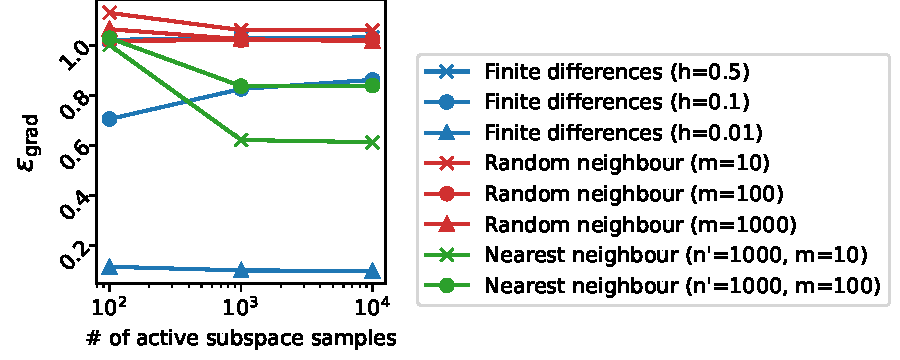
\includegraphics[width=\textwidth]{graphics/ishigami_as_grad_errors}
\delimit
	\caption{Average gradient approximation errors of all used gradient approximation methods over 10 iterations.}
	\label{fig:ishigami_as_grad}
\end{figure}
\end{mdframed}
%
As seen on the left in \cref{fig:ishigami_as_grad}, the finite differences approximation error converges towards zero as the spacing $h$ goes down, which is to be expected.
Furthermore, the nearest neighbour method does deliver better results than the random neighbour method wrt. $\varepsilon_{\mathrm{grad}}$.
The random neighbour methods gradient errors all lie in a range that is even worse compared to the finite differences approximation with a very big step size of $h=5$.

\begin{mdframed}[style=style]
\begin{figure}[H]
\begin{subfigure}{.5\textwidth}
  \centering
   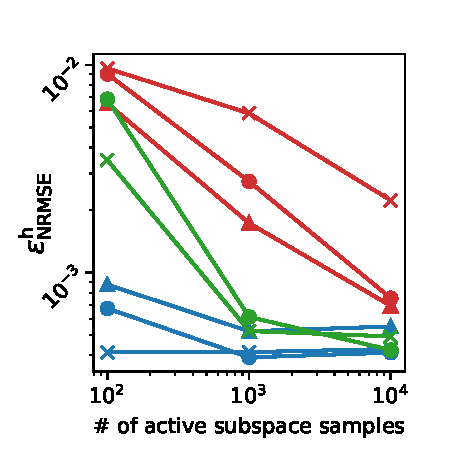
\includegraphics[width=\linewidth]{graphics/ishigami_as_3_inter}
	\caption{Interpolated surrogates with $r=3$.}
	\label{fig:ishigami_as_3_inter}
\end{subfigure}%
\begin{subfigure}{.5\textwidth}
  \centering
   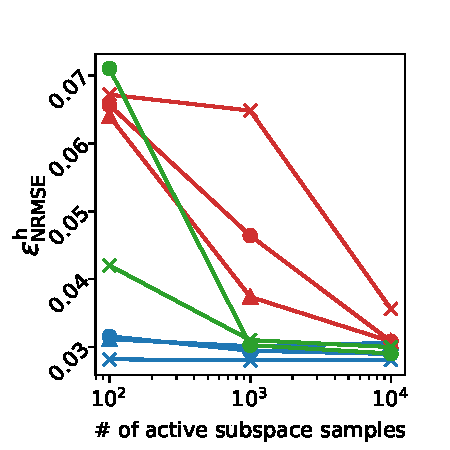
\includegraphics[width=\linewidth]{graphics/ishigami_as_3}
	\caption{Regressed surrogates with $r=3$.}
	\label{fig:ishigami_as_3}
\end{subfigure}
\begin{subfigure}{.5\textwidth}
  \centering
   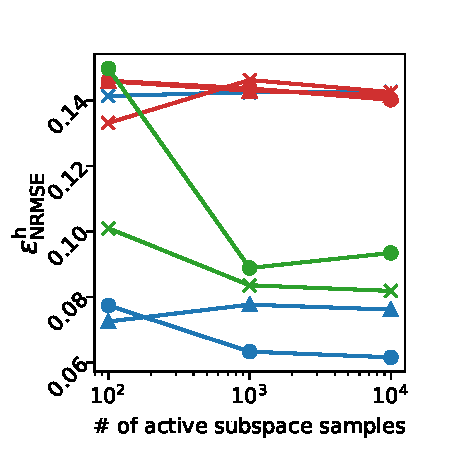
\includegraphics[width=\linewidth]{graphics/ishigami_as_2}
	\caption{Regressed surrogates with $r=2$.}
	\label{fig:ishigami_as_2}
\end{subfigure}
\begin{subfigure}{.5\textwidth}
  \centering
   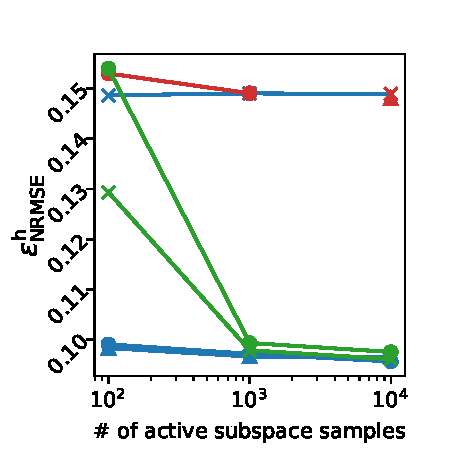
\includegraphics[width=\linewidth]{graphics/ishigami_as_1}
	\caption{Regressed surrogates with $r=1$.}
	\label{fig:ishigami_as_1}
\end{subfigure}
\delimit
	\caption{Gradient approximation error $\varepsilon_{\text{grad}}$ of the previously introduced approximation methods on the left, and the resulting approximation error on the right, computed as the average over 10 iterations.}
	\label{fig:ishigami_as}
\end{figure}
\end{mdframed}
%
\Cref{fig:ishigami_as} shows the actual performance of the different methods by using the look-ahead error.
It can also be observed that the gradient approximation quality from \cref{fig:ishigami_as_grad} does not exactly correlate with the constructed surrogate quality.
While the finite differences method with $h=0.01$ has the best error $\varepsilon_{\mathrm{grad}}$ by far, the constructed surrogate does not perform better than basically the other finite differences methods and also the nearest neighbour methods in \cref{fig:ishigami_as_3_inter} and \cref{fig:ishigami_as_3}.
The random neighbour methods lag a little bit behind in terms of the gradient errors and surrogate errors, but are still in a comparable range to the other methods.
They also take more active subspace samples to converge to the other methods.

In the dimensionality reducing cases \cref{fig:ishigami_as_2} and \cref{fig:ishigami_as_1}, the random neighbour method errors are still contained in a small range with an error comparable to the finite differences approximation with a very big step size of $h=0.5$.
The nearest neighbour method does deliver far better results than the random neighbour method, as it shows a similar quality as the finite differences approximation with smaller step sizes.

These results are good news, as they indicate that approximation methods, which are way cheaper with regards to required function evaluations, can deliver almost the same results as more expensive methods.
For this case, the nearest neighbour method is the preferable approximation method.

\subsection{Random transformations}

To verify the quality of the active subspace method compared to the true optimal linear transformation, which we can't necessarily construct deterministicly with active subspaces, another approach are random linear transformation (see \cref{sec:rt}).
This generation method is not affected by any potential biases or compounding gradient approximation errors like the active subspace method is.
To effectively make use of this strategy, it is vital that we can quickly generate, evaluate, and discard many random transformations, as more generated transformations will allow us to get closer to the potential optimal linear transformation.
As the mainly used transformation evaluator component is forward looking, \ie generating an actual transformed surrogate, we have to employ very lo-fi components to achieve a high transformation count.
We are interested in answering the following questions:
\begin{enumerate}
\item How do the best found random transformations compare to active subspaces?
\item What is the approximation error distribution of the randomly generated transformations?
\item Are random transformations a viable alternative for constructing transformations?
\end{enumerate}
%
Once the algorithm has determined the random transformation with the lowest error based on the lofi surrogates, we construct an actual hifi surrogate and calculate the error again, s.t. we come closer to the approximation real error.
The lo-fi transformation errors are visualized using histograms and while the errors do not come close to the actual hi-fi errors, the distribution of lo-fi errors can provide valuable insight into the actual approximation error distribution, as the lo-fi surrogates should still be comparatively representative.

\begin{mdframed}[style=style]
\begin{figure}[H]
\begin{subfigure}{.5\textwidth}
  \centering
   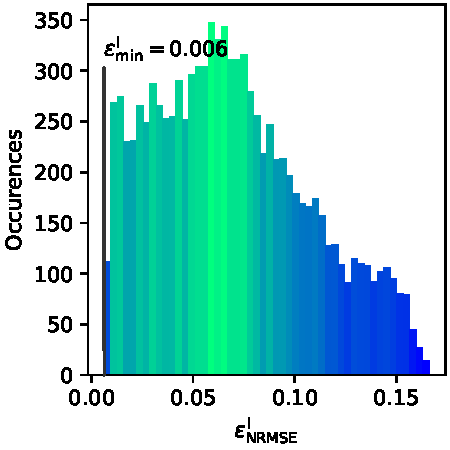
\includegraphics[width=\linewidth]{graphics/ishigami_hist_3_inter}
  \captionof{figure}{Interpolated transformed sparse grid surrogate with $r=3$. The resulting hi-fi error is $\varepsilon^\mathrm{h}_{\mathrm{min}}=0.0007$.}
\vspace{3mm}
  \label{fig:ishigami_hist_3_inter}
\end{subfigure}%
\begin{subfigure}[H]{.5\textwidth}
  \centering
   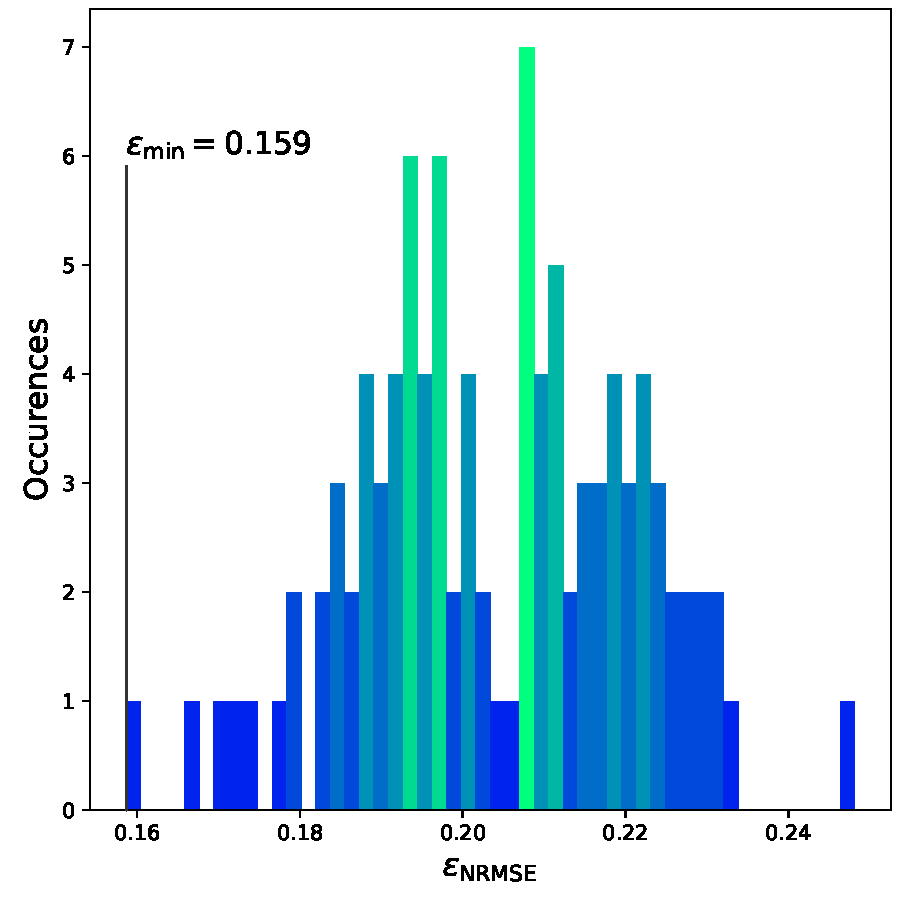
\includegraphics[width=\linewidth]{graphics/ishigami_hist_3}
  \captionof{figure}{Regressed transformed sparse grid surrogate with $r=3$. The resulting hi-fi error is $\varepsilon^\mathrm{h}_{\mathrm{min}}=0.031$.}
\vspace{3mm}
  \label{fig:ishigami_hist_3}
\end{subfigure}
\delimit
  \captionof{figure}{Histogram of lo-fi approximation errors for $10^4$ randomly generated transformations with $r=3$.}
\label{fig:ishigami_hist_3_both}
\end{figure}
\end{mdframed}
%
\Cref{fig:ishigami_hist_3_both} shows the approximation error distribution of interpolation and regression surrogates with $r=3$.
As these histogram errors are calculated using lo-fi surrogates, they are not equal to the hi-fi errors, which are listed in the figure captions.
Comparing these results to the previous transformation results that were achieved with active subspaces, we see that random transformations delivered competitive results.

\begin{mdframed}[style=style]
\vspace{2mm}
\begin{figure}[H]
  \centering
\begin{subfigure}{.5\textwidth}
  \centering
   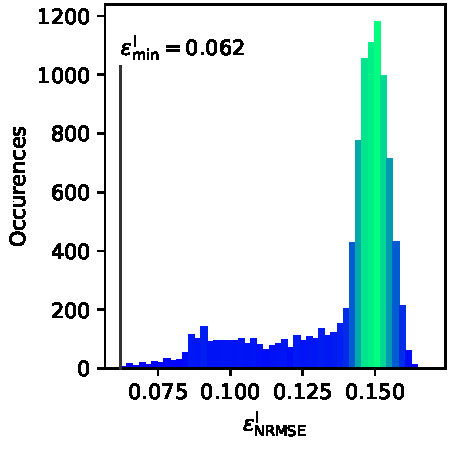
\includegraphics[width=\linewidth]{graphics/ishigami_hist_2}
  \caption{Random transformation approximation error distribution for $r=2$. The resulting hi-fi error is $\varepsilon^\mathrm{h}_{\mathrm{min}}=0.05$.}
\vspace{3mm}
\label{fig:ishigami_hist_2}
\end{subfigure}%
\begin{subfigure}{.5\textwidth}
  \centering
   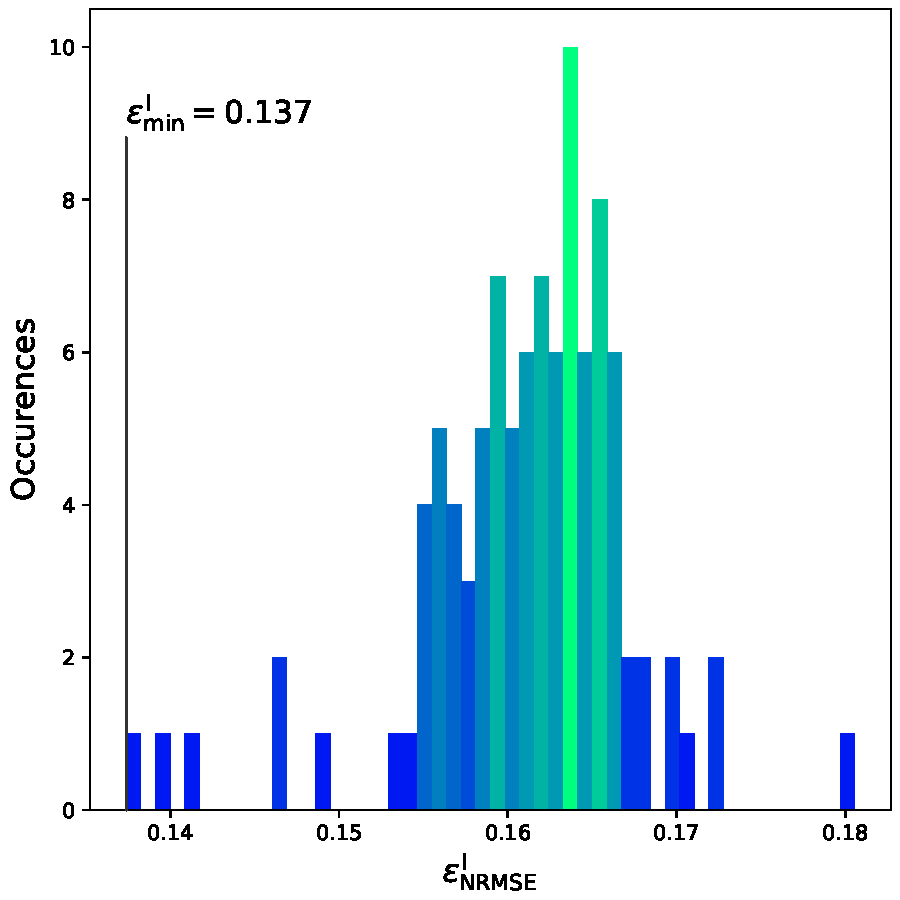
\includegraphics[width=\linewidth]{graphics/ishigami_hist_1}
  \caption{Random transformation approximation error distribution for $r=1$. The resulting hi-fi error is $\varepsilon^\mathrm{h}_{\mathrm{min}}=0.09$.}
\vspace{3mm}
\label{fig:ishigami_hist_1}
\end{subfigure}
\delimit
\caption{Histogram of lo-fi approximation errors for $10^4$ randomly generated dimensionality reducing transformations}
\label{fig:ishigami_hist_12}
\end{figure}
\end{mdframed}
%
\Cref{fig:ishigami_hist_12} shows the lo-fi approximation error distribution of transformed regression surrogates with dimensionality reducing transformations.
Compared to the orientation changing only case from \Cref{fig:ishigami_hist_3_both}, we can see that the distribution has a high peak towards to the tail end of the approximation error range.
As a result, it requires more generation runs to obtain a good transformation, as the probabily of finding one far too the left of the peak is very low.
The best found random transformation still proves to be very competetive compared to active subspaces, as the hi-fi errors are close.

\subsection{Summary}

In conclusion, random transformation generation proves to be a valuable alternative to active subspaces, at least for this example function and enough runs, as it comes close to the active subspace error.
However, for higher dimensional functions, the required amount of random generation iterations to find an acceptable transformation is expected grow very fast, as more dimension will mean more possible directions and also orders of directions.
We can order a set of the same directions in many more ways in higher dimensions.
Therefore, we expect the active subspace method to scale better with higher dimensions as it only requires exactly one run an ordering of directions is implicitly given.

\section{Wing weight function}

Now that we investigated several important pipeline components with regards to a low-dimensional model function, we compare the results to a case with a high-dimensional example model function to look out for properties that can't be generalized from one low-dimensional case study.

Wing weight is 10 dimensional.

TODO: Perform similator evaluations as last section, but focus on differences to low-dimensional case
\chapter{Practical applications}
\label{chap:c8}

\section{Borehole function}
\section{High-dimensional function}
\section{High-dimensional regression}

\chapter{Conclusion and outlook}
\label{chap:c9}

To summarise, we discovered that the transformed sparse grid technique is very flexible in a sense that it can be used as pure black box regression method without the need for additional model function evaluations or gradients, by using the effective neighbour approximation methods as a basis for the active subspace computations.
However, if more information about the model is available, such as the model function itself or its gradients, the technique can also incorporate that additional data to achieve improved results.
The question, for which application the transformed sparse grid technique is most suitable, also warrants further experiments.
While we looked at two major applications, function approximation and regression, in a few experiments, this does not constitute enough evidence to draw definite conclusions.
There are also a few more areas of interest regarding transformed sparse grids that might warrant further research and also potential areas of improvement:

\paragraph{Parallelization}
The implementation of the transformation pipeline has the potential to be almost perfectly parallelized.
A huge portion of the total runtime is spent on evaluating multiple surrogates that either come from transformation stream generators (\cref{sec:tsg}) or from the process of determining the optimal surrogate configuration parameters (\cref{sec:gs}) .
These components can be parallelized by evaluating all of them in parallel, as they don't exchange any data or need to coordinate, using an API like OpenMP \cite{openmp08}.
Furthermore, other optimizations like vectorization \cite{Maleki2011} or GPU execution support with OpenCL \cite{Stone2010} could also be implemented.
This can be combined with the already implemented support of the many of the listed frameworks and technologies by the sparse grid library SG$^{++}$, to obtain a completely optimized and very performant pipeline.

\paragraph{Formalization of concepts}
The main workflow used to eventually come up with the resulting transformation pipeline was mainly based on ideas and practical experiments.
While some formal concepts, like intrinsic dimensionality (\cref{sec:intrinsic}) or active subspaces (\cref{sec:as}), were used, many parts, especially the transformation construction and the iterative algorithm design, were introduced constructively without any proof of their qualities.
Maybe there exist better ways to construct transformed surrogates compared to the ones used in this thesis or a better way to design an iterative transformation algorithm that works with these surrogates.
Therefore, the general ideas of this thesis can be investigated with a more formal and rigorous approach, such that the results are backed by a theory and can be better explained and understood.

\paragraph{Surrogate types}
In this thesis we used sparse grid surrogates as primary reduced surrogates and to a limited degree radial basis function surrogates as well, but mainly as a control method to identify grid specific surrogate properties.
In theory, any surrogate type that uses the tensor-product approach to construct basis functions and supports some form of regression can benefit from the presented linear input transformations.
Another common candidate aside from sparse grids would be the polynomial chaos expansion method \cite{Crestaux2009}.
As the implementation is designed to be very flexible in terms of possible surrogate types, adding support for other methods would not be too difficult.

\paragraph{Lo-fi surrogates}
As mentioned before, it is vital to determine good lo-fi surrogates to guarantee a fast pipeline execution.
Suitable lo-fi surrogates are indicative of the comparative quality of their high fidelity surrogates.
Right now, these are determined more or less empirically, as automating this process is not trivial, epsecially when dealing with pre-convergent behaviour of the lo-fi surrogates.
However, it should be possible to develop an algorithm that automatically determines optimal lo-fi surrogate configuration parameters by generating lo-fi surrogates with different parameters until a representative one is found.
This would make the transformation process even simpler to apply on a variety of models, as it would eliminate prior manual probing of the model function.

\appendix
\chapter{Appendix}

\subsection{B-Spline basis}

One downside of the hat basis is that the functions do not have a continuous derivative.
Instead, there are discontinuities at the grid point $x_{l,i}$ itself where the derivative flips its sign and at the neighbouring grid points $x_{l,i+2}$ and $x_{l,i-2}$ where the derivative changes to zero.
One solution to eliminating these discontinuities are B-Splines, which are just piecewise polynomials.
\begin{definition}[B-Splines]
Let $p \in \mathds{N}$.
Then
\begin{equation}
b^0(x) \coloneqq
\begin{cases}
    1, & x \in [0,1) \\
   0, & \text{else}
\end{cases}
\end{equation}
is a B-Spline of degree $0$ and
\begin{equation}
b^p(x) \coloneqq \frac{1}{p} xb^{p-1}(x) + (p + 1 - x) b^{p-1}(x-1) 
\end{equation}
is a B-Spline of degree $p$.
\end{definition}
This definition of B-Splines is based on the Cox-de-Boor recursion.

\begin{definition}[B-Spline basis functions]
Let $l,i \in \mathds{N}_0$.
Then
\begin{equation}
\phi^b_{l,i}(x) \coloneqq b^p \left( 2^l x + \frac{p+1}{2} -i \right)
\end{equation}
is an univariate B-Spline basis function of degree $p$.
\end{definition}

\subsection{Mod B-Spline basis}

\begin{definition}[Knots]
Let $m,p \in \mathds{N}_0$.
We then define
\begin{equation}
\underline{\xi}=(\xi_0, \dots, \xi_{m + p}) \in \mathds{R}^{m + p}, ~~ \xi_0 \leq \dots \leq \xi_{m + p}
\end{equation}
as a sequence of knots.
\end{definition}

\begin{definition}[B-Splines]
Let $p \in \mathds{N}$.
Then
\begin{equation}
b^0_{i,\underline{\xi}}(x) \coloneqq
\begin{cases}
    1, & x \in [\xi_i,x_i] \\
   0, & \text{else}
\end{cases}
\end{equation}
is a B-Spline of degree $0$ and
\begin{equation}
b_{i,\underline{\xi}}^p(x) \coloneqq \frac{x - \xi_i}{\xi_{i + p} - \xi_i} b_{i,\underline{\xi}}^{p-1}(x) + \frac{\xi_{i+p+1} - \xi_i}{\xi_{i + p} - \xi_i} b_{i+1,\underline{\xi}}^{p-1}(x) 
\end{equation}
is a B-Spline of degree $p$.
\end{definition}

\begin{definition}[Mod B-Spline basis functions]
Let
\begin{equation}
\phi_l^p(x) \coloneqq \sum_{i=0}^{\lceil (p+1)/2 \rceil} (i+1) \phi^p_{l,1-k}(x)
\end{equation}
be the boundary...
\begin{equation}
\phi^{p,\text{mod}}_{l,i}(x) \coloneqq
\begin{cases}
1 &, l=1\\
\phi^p_{l}(x)&, l>1, i=1\\
\phi^p_{l}(x)&, l>1, i=2^l - 1\\
\phi_{l,i}(x)&, \text{else}
\end{cases}
\nonumber
\end{equation}
\end{definition}


\subsection{Modified basis functions}

One method of removing the need of using boundary grid points at least to some degree are modified basis functions.
These basis functions do not require grid points at the boundary.
Instead at every grid level, they extrapolate the values at the boundaries from the grid points closest to the boundaries using a special kind of basis function.
Therefore, it is possible to modify any non-boundary basis $\phi_{l,i}$ by defining the modified basis as follows:
\begin{equation}
\phi^{\text{mod}}_{l,i}(x) \coloneqq
\begin{cases}
1 &, l=1\\
\phi^{\text{left}}_{l}(x)&, l>1, i=1\\
\phi^{\text{right}}_{l}(x)&, l>1, i=2^l - 1\\
\phi_{l,i}(x)&, \text{else}
\end{cases}
\nonumber
\end{equation}
where $\phi^{\text{left}}_{l}$ and $\phi^{\text{right}}_{l}$ are the special boundary extrapolation functions.
Usually $\phi^{\text{left}}_{l}$ and $\phi^{\text{right}}_{l}$ are similar with regards to their structure of the normal basis functions $\phi_{l,i}$, e.g. a hat basis is usually modified with special hat functions.






\subsection{Prewavelets}

A wavelet is a function that has wavelike properties usually with some kind of oscillation around zero.
Many types of wavelet functions are used for signal processing applications because they inhibit some advantageous properties.
One of these properties is the orthogonality property with $\langle \phi_{i},\phi_{j} \rangle = 0$ for all wavelets with $i \neq j$.
Furthermore,  the wavelets are usually discretisized, because it is not possible to analyze a signal using an infinite amount of wavelets.
One wavelet basis that is already used with sparse grids is the so-called mexican hat basis presented in \cite{}, which does not fullfil any orthogonality property.
In fact, using a completely orthogonal basis is quite constraining, i.e. it is not easy to construct a usable orthogonal basis for the context of sparse grids.
However, in the context of sparse grid based ANOVA we can also work with a semi-orthogonal wavelet basis, also called a prewavelet basis.

\begin{definition}[Semi-Orthogonality]
Let $m,n \in \mathds{N}_0, m \neq n$ be two different levels and $\phi_{l,i}$ a basis.
We then call this basis semi-orthogonal if
\begin{align}
\begin{split}
&\langle \phi_{m,i},\phi_{n,j} \rangle = 0
\nonumber
\end{split}
\end{align}
\end{definition}

The basis functions that are used in this thesis are prewavelets with boundary support \cite{GO95,HP17}, which are linear combinations of the hierarchical hat functions $\phi_{l,i}^h(x)$ and have the desirable property of being semi-orthogonal.

\begin{definition}[Boundary prewavelet basis]
The first basis functions are defined as
\begin{equation}
\phi^p_{0,0} = 1\\
\phi^p_{0, 1} = -\phi_{0,0} + \phi_{0,1}\\
\phi^p_{1, 1} = -\phi_{1,0} + \phi_{1,1} -\phi_{1,2}
\end{equation}
For $l \geq 2$ the basis function are defined as 
\begin{equation}
\phi^p_{l,i} = \frac{1}{10} \phi_{l,i-2} - \frac{6}{10} \phi_{l,i-1} + \frac{10}{10} \phi_{l,i} - \frac{6}{10} \phi_{l,i+1} + \frac{1}{10} \phi_{l,i+2}
\label{prewavelet_def}
\end{equation}
with the special boundary cases
\begin{equation}
\phi^p_{l,1} = -\frac{12}{10} \phi_{l,0} + \frac{11}{10} \phi_{l,1} - \frac{6}{10} \phi_{l,2} + \frac{1}{10} \phi_{l,3}\\ \phi^p_{l,2^l-1}(x)=\phi^p_{l,1}(1-x)
\end{equation}
\end{definition}
The multivariate basis functions $\phi^p_{\underline{l},\underline{i}}$ are obtained by applying the tensor-product approach to the univariate basis functions $\phi^p_{l,i}$ to get $\phi^p_{\underline{l},\underline{i}} \coloneqq \prod_{t=1}^{d} \phi^p_{l_t,i_t}$.
These also fullfil the semi-orthogonality with $\langle \phi^p_{\underline{l},\underline{i}},\phi^p_{\underline{l'},\underline{i'}} \rangle = 0$ for $\underline{l} \neq \underline{l'}$.

Test

\newpage
\printbibliography


\pagestyle{empty}
\renewcommand*{\chapterpagestyle}{empty}
\Versicherung
\end{document}
